% ============================================================
% PRN232 - OmniCast project report (English version)
%
% Compile with:
%   xelatex main-en.tex
%   xelatex main-en.tex
% ============================================================
\documentclass[conference,a4paper]{IEEEtran}

% ============================================================
% OmniCast - Shared preamble for IEEEtran conference reports
%   PRN232 (VN / EN) and PRM393 (VN / EN)
% ============================================================

\newif\ifomniEN
\omniENfalse
\newcommand{\bi}[2]{\ifomniEN#2\else#1\fi}

% ---------- Fonts (Windows system fonts, full Vietnamese coverage) ----------
\usepackage{fontspec}
\setmainfont{Times New Roman}
\setsansfont{Arial}
\setmonofont{Consolas}
\XeTeXlinebreaklocale "vi"
\XeTeXlinebreakskip = 0pt plus 1pt

% ---------- Core packages ----------
\usepackage{amsmath}
\usepackage{amssymb}
\usepackage{booktabs}
\usepackage{multirow}
\usepackage{array}
\usepackage{graphicx}
\usepackage{xcolor}
\usepackage{enumitem}
\usepackage{tikz}
\usepackage{listings}
\usepackage{tabularx}
\usepackage{array}
\usepackage{url}
\usepackage{siunitx}
\usepackage[most]{tcolorbox}
\usepackage{fancyhdr}
\usepackage{lastpage}

% ---------- Page numbering & Running headers/footers ----------
\pagestyle{fancy}
\fancyhf{}
\setlength{\headheight}{14pt}
\renewcommand{\headrulewidth}{0.4pt}
\renewcommand{\footrulewidth}{0.4pt}
\fancyhead[L]{\footnotesize\textsf{\bi{OmniCast --- Báo Cáo Kỹ Thuật PRN232 (Mentor: Thầy Huỳnh Vang)}{OmniCast --- PRN232 Technical Report (Mentor: Mr. Huỳnh Vang)}}}
\fancyhead[R]{\footnotesize\textsf{\bi{Học Kỳ Fall 2026 (FA26)}{Fall 2026 Semester (FA26)}}}
\fancyfoot[L]{\footnotesize\textsf{FPTU Quy Nhon AI Campus --- FU Cahata}}
\fancyfoot[R]{\footnotesize\textsf{\textbf{\bi{Trang \thepage\ / \pageref{LastPage}}{Page \thepage\ of \pageref{LastPage}}}}}


\usetikzlibrary{positioning,arrows.meta,shapes.geometric,fit,backgrounds,calc,shadows,decorations.pathmorphing}

% ---------- Hyperref setup ----------
\usepackage{hyperref}
\pdfstringdefDisableCommands{%
  \ifomniEN\def\bi#1#2{#2}\else\def\bi#1#2{#1}\fi
}
\hypersetup{
  colorlinks=true,
  linkcolor=omniBlue,
  citecolor=omniTeal,
  urlcolor=omniPurple,
  pdftitle={OmniCast Project Report - PRN232},
  pdfauthor={Nguyen Binh An, Tran Thanh Son, Nguyen Vinh Phu, Dong Hoang Nguyen},
  pdfsubject={PRN232 - FPTU Quy Nhon AI Campus - FU Cahata},
  pdfkeywords={OmniCast, EPG, broadcast, LiveStream, NestJS, Flutter, Next.js, FPTU Quy Nhon AI Campus, FU Cahata}
}

% ---------- OmniCast brand palette ----------
\definecolor{omniBlue}{HTML}{0E7490}
\definecolor{omniDark}{HTML}{0F172A}
\definecolor{omniTeal}{HTML}{0D9488}
\definecolor{omniPurple}{HTML}{7C3AED}
\definecolor{omniAmber}{HTML}{D97706}
\definecolor{omniRose}{HTML}{E11D48}
\definecolor{omniSlate}{HTML}{475569}
\definecolor{omniLight}{HTML}{F1F5F9}
\definecolor{omniBorder}{HTML}{CBD5E1}

% ---------- Typography tweaks ----------
\renewcommand{\familydefault}{\rmdefault}
\setlength{\parindent}{1em}
\setlength{\parskip}{0pt}
\renewcommand{\arraystretch}{1.12}
\setcounter{secnumdepth}{3}

% ---------- Caption / listing labels ----------
\newcommand{\figName}{Fig.}
\newcommand{\tabName}{TABLE}
\renewcommand{\figurename}{\figName}
\renewcommand{\tablename}{\tabName}
\providecommand{\lstlistname}{Listing}
\renewcommand{\lstlistname}{Listing}

% ---------- Code listings ----------
\lstdefinestyle{omnicode}{
  backgroundcolor=\color{omniLight},
  basicstyle=\ttfamily\footnotesize,
  keywordstyle=\color{omniBlue}\bfseries,
  stringstyle=\color{omniTeal},
  commentstyle=\color{omniSlate}\itshape,
  numbers=left,
  numberstyle=\tiny\color{omniSlate},
  numbersep=6pt,
  frame=leftline,
  framerule=1.2pt,
  rulecolor=\color{omniBorder},
  breaklines=true,
  breakatwhitespace=true,
  tabsize=2,
  showstringspaces=false,
  columns=fullflexible,
  keepspaces=true,
  xleftmargin=10pt,
  framexleftmargin=8pt,
  captionpos=b
}
\lstset{style=omnicode}

% ---------- TikZ shared styles ----------
\tikzset{
  omniNode/.style={
    draw=omniBorder, fill=white, rounded corners=2pt,
    minimum height=9mm, align=center, font=\footnotesize,
    inner sep=4pt, drop shadow={shadow xshift=0.4pt, shadow yshift=-0.4pt, opacity=0.12}
  },
  omniAccent/.style={omniNode, draw=omniBlue, fill=omniBlue!10, line width=0.8pt},
  omniTealNode/.style={omniNode, draw=omniTeal, fill=omniTeal!10},
  omniAmberNode/.style={omniNode, draw=omniAmber, fill=omniAmber!12},
  omniPurpleNode/.style={omniNode, draw=omniPurple, fill=omniPurple!10},
  omniRoseNode/.style={omniNode, draw=omniRose, fill=omniRose!10},
  omniDarkNode/.style={omniNode, draw=omniDark, fill=omniDark!8},
  omniFlow/.style={-{Latex[length=2.2mm]}, line width=0.7pt, draw=omniSlate},
  omniFlowAccent/.style={-{Latex[length=2.2mm]}, line width=0.9pt, draw=omniBlue},
  omniFlowTeal/.style={-{Latex[length=2.2mm]}, line width=0.9pt, draw=omniTeal},
  omniFlowAmber/.style={-{Latex[length=2.2mm]}, line width=0.9pt, draw=omniAmber},
  omniFlowRose/.style={-{Latex[length=2.2mm]}, line width=0.9pt, draw=omniRose},
  omniLabel/.style={font=\scriptsize\itshape, text=omniSlate}
}

% ---------- Info boxes (tcolorbox) ----------
\newtcolorbox{infobox}[1]{
  enhanced, breakable,
  colback=omniLight!60, colframe=omniBlue,
  fonttitle=\bfseries\small, title={#1},
  boxrule=0.6pt, arc=2pt,
  left=5pt, right=5pt, top=3pt, bottom=3pt
}

\newtcolorbox{warnbox}[1]{
  enhanced, breakable,
  colback=omniAmber!8, colframe=omniAmber,
  fonttitle=\bfseries\small, title={#1},
  boxrule=0.6pt, arc=2pt,
  left=5pt, right=5pt, top=3pt, bottom=3pt
}

\newtcolorbox{keybox}[1]{
  enhanced, breakable,
  colback=omniTeal!7, colframe=omniTeal,
  fonttitle=\bfseries\small, title={#1},
  boxrule=0.6pt, arc=2pt,
  left=5pt, right=5pt, top=3pt, bottom=3pt
}

% ---------- Convenience macros ----------
\newcommand{\omnitag}[1]{\textcolor{omniBlue}{\textbf{#1}}}
\newcommand{\code}[1]{\texttt{\small #1}}
\newcommand{\filepath}[1]{\textcolor{omniSlate}{\textit{\small #1}}}
\newcommand{\vn}[1]{#1}

% ---------- Width fitting ----------
\newcommand{\fitcol}[1]{\resizebox{\columnwidth}{!}{#1}}
\newcommand{\fitfull}[1]{\resizebox{\textwidth}{!}{#1}}

\omniENtrue

% English caption labels
\renewcommand{\figName}{Figure}
\renewcommand{\tabName}{Table}
\renewcommand{\lstlistname}{Listing}

% ============================================================
% OmniCast - Shared TikZ figures (bilingual)
%
% Every visible string uses \bi{Vietnamese}{English} so the same
% source renders correctly in both the VN and the EN report.
%
% Requires the OmniCast preamble (omnicast-preamble-ieee.tex) for
% the colour palette, TikZ styles and the \bi macro.
% ============================================================

% ------------------------------------------------------------
% Figure: Overall layered architecture (PRN232)
% ------------------------------------------------------------
\newcommand{\figArchitecture}{%
\begin{tikzpicture}[scale=0.92, transform shape]
  % --- Presentation layer ---
  \node[omniNode, fill=omniPurple!8, draw=omniPurple] (web) at (0,4.6) {\textbf{Next.js 15 Web Portal}\\App Router $\cdot$ React 19\\Tailwind Cinema Dark};
  \node[omniNode, fill=omniPurple!8, draw=omniPurple] (mob) at (4.0,4.6) {\textbf{Flutter 3.x Mobile}\\BLoC $\cdot$ Dio $\cdot$ Sqflite};

  % --- API layer ---
  \node[omniAccent, minimum width=5.4cm, minimum height=1.5cm] (api) at (2.0,2.5) {\textbf{NestJS 10 REST API}\\19 modules $\cdot$ 140+ endpoints\\JWT + RBAC $\cdot$ Swagger/OpenAPI};
  \node[omniTealNode] (gw) at (2.0,0.9) {\textbf{WebSocket Gateway}\\namespace \texttt{/live}\\Socket.IO $\cdot$ WebRTC signalling};
  \node[omniTealNode] (grpc) at (5.6,0.9) {\textbf{gRPC Client}\\AuditLogger proto};

  % --- Microservice ---
  \node[omniAmberNode] (audit) at (5.6,-0.9) {\textbf{Audit-Logger Microservice}\\NestJS $\cdot$ gRPC server\\Render/own deployment};

  % --- Data layer ---
  \node[omniDarkNode, minimum width=3.0cm] (db) at (0.2,-0.9) {\textbf{PostgreSQL}\\Supabase\\21 Prisma models};
  \node[omniDarkNode] (media) at (2.8,-0.9) {\textbf{MediaMTX}\\WHIP ingest\\HLS / WebRTC out};
  \node[omniDarkNode] (cdn) at (5.0,-0.9) {\textbf{Cloudinary}\\media assets};
  \node[omniDarkNode] (ext) at (7.2,-0.9) {\textbf{External APIs}\\OpenAI $\cdot$ TMDB\\YouTube/Twitch/RSS};

  % --- Flows ---
  \draw[omniFlowAccent] (web) -- (api);
  \draw[omniFlowAccent] (mob) -- (api);
  \draw[omniFlow] (api) -- (gw);
  \draw[omniFlow] (api) -- (grpc);
  \draw[omniFlowTeal] (grpc) -- (audit);
  \draw[omniFlow] (api) -- (db);
  \draw[omniFlow] (api) -- (media);
  \draw[omniFlow] (api) -- (cdn);
  \draw[omniFlowAmber] (api) -- (ext);
  \draw[omniFlow] (media) -- (mob);
  \draw[omniFlow] (media) -- (web);

  % --- Layer annotations ---
  \node[omniLabel, anchor=west] at (-1.85,4.6) {\bi{\textbf{Tầng}}{\textbf{Presentation}}};
  \node[omniLabel, anchor=west] at (-1.85,2.5) {\bi{\textbf{API}}{\textbf{API}}};
  \node[omniLabel, anchor=west] at (-1.85,0.9) {\bi{\textbf{Real-time}}{\textbf{Real-time}}};
  \node[omniLabel, anchor=west] at (-1.85,-0.9) {\bi{\textbf{Dữ liệu}}{\textbf{Data}}};
\end{tikzpicture}%
}

% ------------------------------------------------------------
% Figure: EPG anti-conflict scheduling timeline
% ------------------------------------------------------------
\newcommand{\figScheduleConflict}{%
\begin{tikzpicture}[x=0.95cm, y=0.75cm]
  % Existing event on the channel
  \filldraw[fill=omniBlue!22, draw=omniBlue, line width=0.8pt]
    (1.0,1.6) rectangle (5.2,2.3);
  \node at (3.1,1.95) {\footnotesize \bi{\textbf{Sự kiện đã có}}{\textbf{Existing event}} (14:00--15:00)};

  % Candidate event - overlapping head
  \filldraw[fill=omniRose!20, draw=omniRose, line width=0.8pt]
    (0.4,0.45) rectangle (4.2,1.15);
  \node at (2.3,0.8) {\footnotesize \bi{\textbf{Lịch mới}}{\textbf{New schedule}} (13:30--14:30)};
  \node[omniRose, font=\scriptsize\bfseries] at (2.3,0.15) {\bi{giao thoa đầu $\rightarrow$ 409}{head overlap $\rightarrow$ 409}};

  % Candidate event - overlapping tail
  \filldraw[fill=omniRose!20, draw=omniRose, line width=0.8pt]
    (4.0,2.85) rectangle (7.2,3.55);
  \node at (5.6,3.2) {\footnotesize \bi{\textbf{Lịch mới}}{\textbf{New schedule}} (14:30--15:30)};
  \node[omniRose, font=\scriptsize\bfseries] at (5.6,2.6) {\bi{giao thoa đuôi $\rightarrow$ 409}{tail overlap $\rightarrow$ 409}};

  % Candidate event - fully contained
  \filldraw[fill=omniRose!20, draw=omniRose, line width=0.8pt]
    (0.9,3.4) rectangle (5.6,4.1);
  \node at (3.25,3.75) {\footnotesize \bi{\textbf{Lịch mới}}{\textbf{New schedule}} (13:00--16:00)};
  \node[omniRose, font=\scriptsize\bfseries] at (3.25,3.15) {\bi{bao trùm toàn bộ $\rightarrow$ 409}{fully contained $\rightarrow$ 409}};

  % Non-overlapping on another channel
  \filldraw[fill=omniTeal!20, draw=omniTeal, line width=0.8pt]
    (6.0,0.45) rectangle (9.4,1.15);
  \node at (7.7,0.8) {\footnotesize \bi{\textbf{Kênh khác}}{\textbf{Other channel}} (14:00--15:00)};
  \node[omniTeal, font=\scriptsize\bfseries] at (7.7,0.15) {\bi{cho phép $\rightarrow$ 201}{allowed $\rightarrow$ 201}};

  % Time axis
  \draw[-{Latex[length=2mm]}, line width=0.6pt] (0.2,0) -- (9.8,0);
  \foreach \x/\lab in {1.0/13:00,2.6/14:00,4.2/15:00,5.8/16:00,7.4/17:00,9.0/18:00}{
    \draw (\x,0) -- (\x,0.12);
    \node[font=\scriptsize, below=2pt] at (\x,0) {\lab};
  }
\end{tikzpicture}%
}

% ------------------------------------------------------------
% Figure: AI Curator pipeline (consolidated single call + fallback)
% ------------------------------------------------------------
\newcommand{\figAiPipeline}{%
\begin{tikzpicture}[node distance=0.9cm and 1.3cm]
  \node[omniNode] (input) {\bi{\textbf{Đầu vào}}{\textbf{Input}}\\title + description\\category + tags};
  \node[omniAccent, right=of input] (norm) {\bi{\textbf{Chuẩn hoá}}{\textbf{Normalise}}\\\texttt{CuratorProgramInput}};
  \node[omniAmberNode, right=of norm] (branch) {\bi{\textbf{Phân nhánh}}{\textbf{Branch}}\\\bi{có \texttt{OPENAI\_API\_KEY}?}{has \texttt{OPENAI\_API\_KEY}?}};

  \node[omniTealNode, above right=0.4cm and 1.6cm of branch] (prompt) {\textbf{buildConsolidatedPrompt}\\temperature 0.3 $\cdot$ top\_p 0.95};
  \node[omniTealNode, right=of prompt] (call) {\bi{\textbf{Gọi OpenAI}}{\textbf{Call OpenAI}}\\gpt-4o $\cdot$ retry + backoff};
  \node[omniDarkNode, right=of call] (valid) {\bi{\textbf{Kiểm tra schema}}{\textbf{Schema check}}\\Zod validate};

  \node[omniRoseNode, below right=0.4cm and 1.6cm of branch] (fallback) {\bi{\textbf{Heuristic fallback}}{\textbf{Heuristic fallback}}\\\texttt{sentiment / compliance / editorial}};
  \node[omniPurpleNode, right=of fallback] (conf) {\bi{\textbf{Tính confidence}}{\textbf{Compute confidence}}\\heuristic $\cdot$ clamp 0..1};

  \node[omniAccent, right=of valid, minimum width=2.4cm] (report) {\textbf{AiCuratorReport}\\\bi{\texttt{lưu trong PostgreSQL}}{\texttt{stored in PostgreSQL}}};
  \node[omniNode, below=of report] (stamp) {\bi{\textbf{Dấu vết}}{\textbf{Provenance}}\\\texttt{promptVersion} $\cdot$ \texttt{aiModelVersion}\\\texttt{openaiCallMs} $\cdot$ \texttt{openaiRetries}};

  \draw[omniFlowAccent] (input) -- (norm);
  \draw[omniFlowAccent] (norm) -- (branch);
  \draw[omniFlowTeal] (branch) -- node[above, font=\scriptsize] {\bi{có}{yes}} (prompt);
  \draw[omniFlowTeal] (prompt) -- (call);
  \draw[omniFlowTeal] (call) -- (valid);
  \draw[omniFlowRose] (branch) -- node[below, font=\scriptsize] {\bi{không}{no}} (fallback);
  \draw[omniFlowRose] (fallback) -- (conf);
  \draw[omniFlowTeal] (valid) -- (report);
  \draw[omniFlowRose] (conf) -- (report);
  \draw[omniFlow] (report) -- (stamp);
  \draw[omniFlowRose, dashed] (valid) to[out=200,in=20] node[font=\scriptsize, text=omniRose] {validate fail} (fallback);
\end{tikzpicture}%
}

% ------------------------------------------------------------
% Figure: Mobile BLoC layered architecture (PRM393)
% ------------------------------------------------------------
\newcommand{\figMobileArchitecture}{%
\begin{tikzpicture}[scale=0.95, transform shape]
  \begin{scope}[local bounding box=pres]
    \node[omniPurpleNode, minimum width=5.0cm, minimum height=1.4cm] (pres) at (0,3.4) {\bi{\textbf{Tầng Presentation}}{\textbf{Presentation layer}}\\31 screens $\cdot$ 22 widgets\\GoRouter navigation};
  \end{scope}

  \begin{scope}[local bounding box=logic]
    \node[omniAccent, minimum width=5.0cm, minimum height=1.4cm] (logic) at (0,1.5) {\bi{\textbf{Tầng Logic (BLoC)}}{\textbf{Logic layer (BLoC)}}\\12 BLoC/Cubit\\events $\rightarrow$ states};
  \end{scope}

  \begin{scope}[local bounding box=data]
    \node[omniTealNode, minimum width=5.0cm, minimum height=1.4cm] (data) at (0,-0.4) {\bi{\textbf{Tầng Data}}{\textbf{Data layer}}\\10 repositories $\cdot$ 10 models\\Dio client $\cdot$ AuthInterceptor};
  \end{scope}

  \begin{scope}[local bounding box=core]
    \node[omniDarkNode, minimum width=5.0cm, minimum height=1.4cm] (core) at (0,-2.3) {\bi{\textbf{Tầng Core}}{\textbf{Core layer}}\\DI (get\_it) $\cdot$ theme $\cdot$ i18n\\constants $\cdot$ utils $\cdot$ services};
  \end{scope}

  \node[omniAmberNode, right=1.4cm of data] (local) {\bi{\textbf{Lưu trữ cục bộ}}{\textbf{Local Storage}}\\\texttt{omnicast\_local.db}\\Sqflite offline-first};
  \node[omniRoseNode, right=1.4cm of core] (remote) {\bi{\textbf{Từ xa}}{\textbf{Remote}}\\REST API (NestJS)\\FCM push $\cdot$ Supabase Realtime};

  \draw[omniFlowAccent] (pres) -- node[right, font=\scriptsize] {dispatch} (logic);
  \draw[omniFlowAccent] (logic) -- node[right, font=\scriptsize] {\bi{gọi}{calls}} (data);
  \draw[omniFlowTeal] (data) -- (local);
  \draw[omniFlowRose] (data) -- (remote);
  \draw[omniFlow, dashed] (core) -- (data);
\end{tikzpicture}%
}

% ------------------------------------------------------------
% Figure: Offline-first watchlist sync flow
% ------------------------------------------------------------
\newcommand{\figOfflineSync}{%
\begin{tikzpicture}[node distance=1.0cm and 1.4cm]
  \node[omniNode] (ui) {\textbf{WatchlistScreen}\\SaveToWatchlistButton};
  \node[omniAccent, right=of ui] (bloc) {\textbf{WatchlistBloc}\\\texttt{AddToWatchlist}\\\texttt{LoadWatchlist}};
  \node[omniTealNode, right=of bloc] (repo) {\textbf{WatchlistRepository}};

  \node[omniAmberNode, below=of repo] (sqlite) {\textbf{SQLite}\\\texttt{omnicast\_local.db}\\\texttt{WatchlistCache}};
  \node[omniRoseNode, right=of sqlite] (api) {\textbf{REST}\\\texttt{GET/POST /me/watchlist}};
  \node[omniDarkNode, right=of api] (notif) {\bi{\textbf{Thông báo cục bộ}}{\textbf{Local notification}}\\\bi{đặt lịch trước 15 phút}{schedule 15 min ahead}};

  \draw[omniFlowAccent] (ui) -- (bloc);
  \draw[omniFlowAccent] (bloc) -- (repo);
  \draw[omniFlowTeal] (repo) -- (sqlite);
  \draw[omniFlowRose] (repo) -- (api);
  \draw[omniFlow] (sqlite) -- (notif);
  \draw[omniFlowRose, dashed] (api) to[out=0,in=180] node[above, font=\scriptsize] {\bi{đồng bộ khi online}{sync online}} (sqlite);
  \draw[omniFlowAmber, dashed] (sqlite) to[out=200,in=20] node[below, font=\scriptsize, text=omniAmber] {\bi{đọc offline khi mất mạng}{read offline when offline}} (ui);
\end{tikzpicture}%
}

% ------------------------------------------------------------
% Figure: CI/CD pipeline
% ------------------------------------------------------------
\newcommand{\figCicd}{%
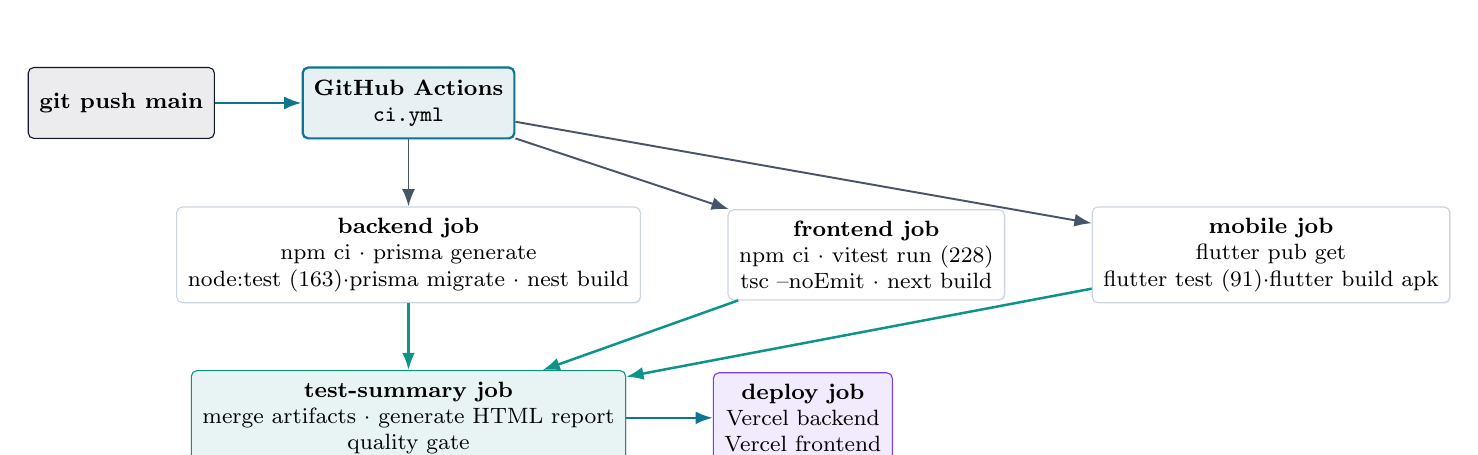
\begin{tikzpicture}[node distance=0.85cm and 1.1cm]
  \node[omniDarkNode] (push) {\textbf{git push main}};
  \node[omniAccent, right=of push] (gha) {\textbf{GitHub Actions}\\\texttt{ci.yml}};

  \node[omniNode, below=of gha] (be) {\bi{\textbf{backend job}}{\textbf{backend job}}\\npm ci $\cdot$ prisma generate\\node:test (163)$\cdot$prisma migrate $\cdot$ nest build};
  \node[omniNode, right=of be] (fe) {\bi{\textbf{frontend job}}{\textbf{frontend job}}\\npm ci $\cdot$ vitest run (228)\\tsc --noEmit $\cdot$ next build};
  \node[omniNode, right=of fe] (mob) {\bi{\textbf{mobile job}}{\textbf{mobile job}}\\flutter pub get\\flutter test (91)$\cdot$flutter build apk};

  \node[omniTealNode, below=of be] (sum) {\bi{\textbf{test-summary job}}{\textbf{test-summary job}}\\merge artifacts $\cdot$ generate HTML report\\quality gate};
  \node[omniPurpleNode, right=of sum] (dep) {\bi{\textbf{deploy job}}{\textbf{deploy job}}\\Vercel backend\\Vercel frontend};

  \draw[omniFlowAccent] (push) -- (gha);
  \draw[omniFlow] (gha) -- (be);
  \draw[omniFlow] (gha) -- (fe);
  \draw[omniFlow] (gha) -- (mob);
  \draw[omniFlowTeal] (be) -- (sum);
  \draw[omniFlowTeal] (fe) -- (sum);
  \draw[omniFlowTeal] (mob) -- (sum);
  \draw[omniFlowAccent] (sum) -- (dep);
\end{tikzpicture}%
}

% ------------------------------------------------------------
% Figure: JWT authentication & RBAC flow
% ------------------------------------------------------------
\newcommand{\figAuthFlow}{%
\begin{tikzpicture}[node distance=0.9cm and 1.2cm]
  \node[omniNode] (client) {\bi{\textbf{Client}}{\textbf{Client}}\\\bi{Web hoặc Mobile}{Web or Mobile}};
  \node[omniAccent, right=of client] (auth) {\textbf{AuthController}\\\texttt{/api/v1/auth/login}};
  \node[omniTealNode, right=of auth] (svc) {\textbf{AuthService}\\bcrypt verify\\deactivated check};
  \node[omniDarkNode, right=of svc] (db) {\textbf{PostgreSQL}\\\texttt{User} + \texttt{RefreshToken}};

  \node[omniPurpleNode, below=of svc] (tok) {\bi{\textbf{Cấp token}}{\textbf{Issue tokens}}\\\texttt{access} 60 min\\\texttt{refresh} 90 days (rotated)};
  \node[omniAmberNode, right=of tok] (guard) {\bi{\textbf{RBAC Guards}}{\textbf{RBAC Guards}}\\\texttt{JwtAuthGuard}\\\texttt{RolesGuard}};
  \node[omniRoseNode, right=of guard] (api) {\bi{\textbf{Endpoint có kiểm tra quyền}}{\textbf{Role-guarded endpoint}}\\\texttt{@Roles(1,2,3)}};

  \draw[omniFlowAccent] (client) -- (auth);
  \draw[omniFlowAccent] (auth) -- (svc);
  \draw[omniFlow] (svc) -- (db);
  \draw[omniFlowTeal] (svc) -- (tok);
  \draw[omniFlowTeal] (tok) -- (guard);
  \draw[omniFlowRose] (guard) -- (api);
  \draw[omniFlow, dashed] (client) to[out=0,in=180] node[above, font=\scriptsize] {Bearer token} (guard);
\end{tikzpicture}%
}

% ------------------------------------------------------------
% Figure: Ingest pipeline (external sources -> normalised events)
% ------------------------------------------------------------
\newcommand{\figIngest}{%
\begin{tikzpicture}[node distance=0.85cm and 1.2cm]
  \node[omniAmberNode] (yt) {\textbf{YouTube}\\Data API v3};
  \node[omniAmberNode, below=of yt] (tw) {\textbf{Twitch}\\Helix API};
  \node[omniAmberNode, below=of tw] (rss) {\textbf{RSS}\\Feed parser};

  \node[omniAccent, right=of yt] (cron) {\bi{\textbf{Bộ lập lịch}}{\textbf{Scheduler}}\\\texttt{@Cron}\\\bi{15'/30' phút}{15'/30' minutes}};
  \node[omniTealNode, right=of cron] (norm) {\bi{\textbf{Chuẩn hoá}}{\textbf{Normalise}}\\\texttt{NormalizedLiveEvent}\\duration in seconds};
  \node[omniDarkNode, right=of norm] (db) {\textbf{LiveEvent}\\\bi{upsert theo kênh}{upsert per channel}};
  \node[omniRoseNode, right=of db] (fill) {\bi{\textbf{Điền lịch trống}}{\textbf{EPG filler}}\\24/7 grid};

  \draw[omniFlowAmber] (yt) -- (cron);
  \draw[omniFlowAmber] (tw) -- (cron);
  \draw[omniFlowAmber] (rss) -- (cron);
  \draw[omniFlowAccent] (cron) -- (norm);
  \draw[omniFlowTeal] (norm) -- (db);
  \draw[omniFlowRose] (db) -- (fill);
\end{tikzpicture}%
}

% ------------------------------------------------------------
% Figure: End-to-End LiveStream & Live Studio Real-Time Architecture
% ------------------------------------------------------------
\newcommand{\figLiveStreamArch}{%
\begin{tikzpicture}[node distance=0.75cm and 1.1cm]
  % --- Broadcaster / Studio Sources (Left) ---
  \node[omniPurpleNode, minimum width=3.4cm] (tab1) at (0, 3.3) {\bi{\textbf{Tab 1: Chọn nội dung}}{\textbf{Tab 1: Curated Live}}\\VOD Library $\cdot$ Anti-piracy guard};
  \node[omniPurpleNode, minimum width=3.4cm] (tab2) at (0, 1.9) {\bi{\textbf{Tab 2: Tự ghi hình / Camera}}{\textbf{Tab 2: Self-Record / Camera}}\\WHIP WebRTC $\cdot$ Screen $\cdot$ Dropzone};
  \node[omniPurpleNode, minimum width=3.4cm] (tab3) at (0, 0.5) {\bi{\textbf{Tab 3: Kho công khai}}{\textbf{Tab 3: Public Catalog}}\\Verified HLS/MP4 $\cdot$ HEAD probe};
  \node[omniPurpleNode, minimum width=3.4cm] (tab4) at (0,-0.9) {\bi{\textbf{Tab 4: Điều hành \& Tương tác}}{\textbf{Tab 4: Host Control Console}}\\Pinned announcement $\cdot$ Stop/Switch};

  % --- Ingestion & Orchestration (Middle-Left) ---
  \node[omniAccent, minimum width=3.8cm, minimum height=1.5cm] (studio) at (4.6, 2.2) {\textbf{LiveStudioService}\\atomic event lifecycle\\\texttt{switchProgramOnLiveEvent}};
  \node[omniDarkNode, minimum width=3.8cm] (mtx) at (4.6, 0.5) {\textbf{MediaMTX + Cloudinary}\\WHIP/RTSP $\rightarrow$ WHEP/HLS (\texttt{.m3u8})\\Direct Drive proxy $\cdot$ Signed upload};
  \node[omniTealNode, minimum width=3.8cm, minimum height=1.5cm] (ws) at (4.6,-1.1) {\textbf{LiveStreamGateway (\texttt{/live})}\\Socket.IO rooms (\texttt{event:id})\\WebRTC SDP/ICE signalling};

  % --- Real-Time Events & Viewer Rooms (Right) ---
  \node[omniAmberNode, minimum width=4.0cm] (webroom) at (9.6, 2.5) {\bi{\textbf{Phòng Live Web (\texttt{/live/[id]})}}{\textbf{Web Live Room (\texttt{/live/[id]})}}\\7 genre lounges $\cdot$ Cinema mode\\Lineup switcher $\cdot$ Join Lobby};
  \node[omniAmberNode, minimum width=4.0cm] (mobroom) at (9.6, 0.7) {\bi{\textbf{Màn hình Mobile (\texttt{LiveWatch})}}{\textbf{Mobile \texttt{LiveWatchScreen}}}\\OmniPlayer $\cdot$ LAN host discovery\\Zero-cartoon exponential retry};
  \node[omniRoseNode, minimum width=4.0cm] (ops) at (9.6,-1.1) {\bi{\textbf{Thao tác Tương tác Tức thời}}{\textbf{Interactive Live Operations}}\\Chat \& Reply $\cdot$ 0ms Haptic Reactions\\6-Tier Super Chat $\cdot$ Host Toast};

  % --- Flows ---
  \draw[omniFlowAccent] (tab1) -- (studio);
  \draw[omniFlowAccent] (tab2) -- (studio);
  \draw[omniFlow] (tab2) -- (mtx);
  \draw[omniFlowAccent] (tab3) -- (studio);
  \draw[omniFlowTeal] (tab4) -- (ws);
  \draw[omniFlowTeal] (studio) -- (ws);
  \draw[omniFlow] (studio) -- (mtx);
  \draw[omniFlowAccent] (mtx) -- (webroom);
  \draw[omniFlowAccent] (mtx) -- (mobroom);
  \draw[omniFlowTeal] (ws) -- (webroom);
  \draw[omniFlowTeal] (ws) -- (mobroom);
  \draw[omniFlowRose] (ws) -- (ops);
  \draw[omniFlowRose, dashed] (ops) -- (mobroom);
  \draw[omniFlowRose, dashed] (ops) -- (webroom);
\end{tikzpicture}%
}

% ------------------------------------------------------------
% Figure: 5-Domain Relational Database Architecture (21 Prisma Models)
% ------------------------------------------------------------
\newcommand{\figDatabaseArchitecture}{%
\begin{tikzpicture}[node distance=0.8cm and 1.0cm]
  \node[omniAccent, minimum width=3.6cm, minimum height=2.1cm] (d1) at (0, 2.2) {\bi{\textbf{1. Định danh \& Bảo mật}}{\textbf{1. Identity \& Security}}\\\texttt{User} $\cdot$ \texttt{Role}\\\texttt{RefreshToken}};
  \node[omniTealNode, minimum width=4.0cm, minimum height=2.1cm] (d2) at (4.4, 2.2) {\bi{\textbf{2. Lõi Phát sóng \& EPG}}{\textbf{2. Broadcast Core \& EPG}}\\\texttt{Channel} $\cdot$ \texttt{Program}\\\texttt{Schedule} $\cdot$ \texttt{LiveEvent}\\\texttt{Category} $\cdot$ \texttt{ProgramCategory}};
  \node[omniPurpleNode, minimum width=4.0cm, minimum height=2.1cm] (d3) at (9.0, 2.2) {\bi{\textbf{3. Tương tác \& Thương mại}}{\textbf{3. Social \& Monetization}}\\\texttt{Comment} $\cdot$ \texttt{Reaction} $\cdot$ \texttt{Donation}\\\texttt{SubscriptionPlan} $\cdot$ \texttt{UserSubscription}\\\texttt{Watchlist} $\cdot$ \texttt{ViewHistory} $\cdot$ \texttt{FavoriteChannel}};
  \node[omniAmberNode, minimum width=4.2cm, minimum height=1.8cm] (d4) at (2.2,-0.5) {\bi{\textbf{4. Vận hành \& Kiểm toán gRPC}}{\textbf{4. Operations \& gRPC Audit}}\\\texttt{Notification} $\cdot$ \texttt{AuditLog}\\\texttt{WebhookSubscription}};
  \node[omniRoseNode, minimum width=4.2cm, minimum height=1.8cm] (d5) at (7.2,-0.5) {\bi{\textbf{5. Trí tuệ Nhân tạo (AI Curator)}}{\textbf{5. AI Content Intelligence}}\\\texttt{AiCuratorReport}\\\bi{1-1 với \texttt{Program} (sentiment/compliance)}{1-to-1 with \texttt{Program} (sentiment/compliance)}};

  \draw[omniFlowAccent] (d1) -- (d2);
  \draw[omniFlowTeal] (d2) -- (d3);
  \draw[omniFlow] (d1) -- (d3);
  \draw[omniFlowAmber] (d1) -- (d4);
  \draw[omniFlowRose] (d2) -- (d5);
\end{tikzpicture}%
}

% ------------------------------------------------------------
% Figure: Complete Mobile Navigation & 31-Screen Hierarchy (PRM393)
% ------------------------------------------------------------
\newcommand{\figMobileScreenMap}{%
\begin{tikzpicture}[node distance=0.65cm and 0.9cm]
  \node[omniDarkNode, minimum width=3.6cm] (root) at (4.5, 3.6) {\textbf{GoRouter Root}\\Splash $\cdot$ Onboarding $\cdot$ Auth (4)};

  \node[omniAccent, minimum width=3.8cm] (shell) at (4.5, 2.1) {\textbf{MainNavigationShell (6 Tabs)}\\Home $\cdot$ Channels $\cdot$ Schedule\\Saved $\cdot$ History $\cdot$ Profile};

  \node[omniRoseNode, minimum width=3.5cm] (live) at (0.2, 0.4) {\bi{\textbf{Cụm Xem Live \& VOD}}{\textbf{Live \& VOD Cluster}}\\\texttt{LiveNowScreen} (\texttt{/live})\\\texttt{LiveWatchScreen} (\texttt{/live/:id})\\\texttt{OmniPlayer} + Super Chat + Chat};

  \node[omniPurpleNode, minimum width=3.6cm] (studio) at (4.5, 0.4) {\bi{\textbf{Cụm Studio Phát sóng}}{\textbf{Broadcast Studio Cluster}}\\\texttt{LiveStudioScreen} (4 Tabs)\\\texttt{MobileStudioRecorderScreen}\\Teleprompter $\cdot$ VU Meter $\cdot$ QC};

  \node[omniTealNode, minimum width=3.5cm] (admin) at (8.8, 0.4) {\bi{\textbf{Cụm Quản trị \& AI}}{\textbf{Admin \& AI Cluster}}\\\texttt{AdminManageScreen} (4 Tabs)\\\texttt{AiCuratorScreen} $\cdot$ Schedule Form\\Notifications $\cdot$ Settings $\cdot$ Sub Plans};

  \draw[omniFlowAccent] (root) -- (shell);
  \draw[omniFlowRose] (shell) -- (live);
  \draw[omniFlow] (shell) -- (studio);
  \draw[omniFlowTeal] (shell) -- (admin);
\end{tikzpicture}%
}


\begin{document}

% ============================================================
% PRN232 - Academic Cover Page (Trang Bìa Đồ Án FPT University)
% ============================================================
\onecolumn
\thispagestyle{empty}

\begin{tikzpicture}[remember picture, overlay]
  % Khung viền đôi trang trọng
  \draw[line width=2pt, color=omniDark] 
    ($(current page.north west) + (20mm,-20mm)$) 
    rectangle 
    ($(current page.south east) + (-15mm,20mm)$);
  \draw[line width=0.8pt, color=omniBlue] 
    ($(current page.north west) + (21.5mm,-21.5mm)$) 
    rectangle 
    ($(current page.south east) + (-16.5mm,21.5mm)$);
  \fill[omniBlue] ($(current page.north west) + (21.5mm,-21.5mm)$) circle (2.5pt);
  \fill[omniBlue] ($(current page.north east) + (-16.5mm,-21.5mm)$) circle (2.5pt);
  \fill[omniBlue] ($(current page.south west) + (21.5mm,21.5mm)$) circle (2.5pt);
  \fill[omniBlue] ($(current page.south east) + (-16.5mm,21.5mm)$) circle (2.5pt);
\end{tikzpicture}

\begin{center}
  \vspace*{-7mm}
  {\bfseries\large\bi{BỘ GIÁO DỤC VÀ ĐÀO TẠO}{MINISTRY OF EDUCATION AND TRAINING}}\\[1.5mm]
  {\bfseries\Large\bi{TRƯỜNG ĐẠI HỌC FPT --- FPTU QUY NHON AI CAMPUS}{FPT UNIVERSITY --- FPTU QUY NHON AI CAMPUS}}\\[1.5mm]
  {\small\bfseries\textcolor{omniBlue}{FU CAHATA $\cdot$ \bi{KHOA CÔNG NGHỆ THÔNG TIN --- BỘ MÔN KỸ THUẬT PHẦN MỀM}{FACULTY OF INFORMATION TECHNOLOGY --- SOFTWARE ENGINEERING}}}\\[5mm]

  % Huy hiệu nhận diện hệ thống OmniCast
  \begin{tikzpicture}
    \node[draw=omniBlue, fill=omniLight, rounded corners=6pt, line width=1.2pt, inner sep=6pt] {
      \textbf{\large\textcolor{omniDark}{OMNI}\textcolor{omniBlue}{CAST}}
      \quad\textcolor{omniSlate}{\footnotesize$\vert$}\quad
      \textcolor{omniDark}{\footnotesize\bfseries\bi{NỀN TẢNG PHÁT SÓNG THÔNG MINH}{BROADCAST INTELLIGENCE PLATFORM}}
    };
  \end{tikzpicture}
  \vspace{5mm}

  {\Large\bfseries\bi{BÁO CÁO NGHIỆM THU ĐỒ ÁN HỌC PHẦN}{FINAL PROJECT DELIVERABLE REPORT}}\\[2.5mm]
  {\large\bfseries\bi{HỌC PHẦN: PRN232 --- XÂY DỰNG ỨNG DỤNG PHÍA SAU ĐA NỀN TẢNG}{COURSE: PRN232 --- BUILDING CROSS-PLATFORM BACK-END APPLICATION}}\\[5mm]

  {\color{omniBlue}\rule{0.85\linewidth}{1.6pt}}\\[4mm]
  {\LARGE\bfseries\bi{HỆ THỐNG LẬP LỊCH VÀ PHÁT SÓNG}{OMNICAST: DIGITAL BROADCAST SCHEDULING}}\\[2mm]
  {\LARGE\bfseries\bi{NỘI DUNG SỐ ĐA NỀN TẢNG OMNICAST}{\& DELIVERY SYSTEM}}\\[2.5mm]
  {\large\bfseries\textcolor{omniBlue}{Enterprise Media \& Broadcast Intelligence Network}}\\[2mm]
  {\normalsize\itshape\bi{Kiến trúc NestJS vi dịch vụ gRPC, Cổng Web Next.js 15, Phòng LiveStream \& Studio Thời gian thực, Thuật toán chống xung đột lịch EPG 24/7 và Trợ lý AI Curator}{NestJS gRPC Microservices, Next.js 15 Web Portal, Real-Time LiveStream \& Studio, 24/7 EPG Conflict Detection Algorithm and AI Curation}}\\[3.5mm]
  {\color{omniBlue}\rule{0.85\linewidth}{1.6pt}}\\[5mm]

  \begin{tcolorbox}[
    colback=white, colframe=omniBorder, boxrule=0.8pt, arc=3pt,
    width=0.90\linewidth, left=6mm, right=6mm, top=3.5mm, bottom=3.5mm
  ]
  \renewcommand{\arraystretch}{1.24}
  \footnotesize
  \begin{tabular}{p{4.3cm}p{8.8cm}}
    \textbf{\bi{Giảng viên hướng dẫn (Mentor):}{Mentor / Supervisor:}} & \textbf{\bi{Thầy Huỳnh Vang}{Mr. Huỳnh Vang}} (\bi{Bộ môn Kỹ thuật Phần mềm --- FPTU}{Software Engineering Dept. --- FPTU}) \\
    \textbf{\bi{Đơn vị \& Câu lạc bộ:}{Campus \& Team Note:}}          & \textbf{FPTU Quy Nhon AI Campus --- FU Cahata} \\
    \textbf{\bi{Học kỳ thực hiện:}{Academic Semester:}}                & Fall 2026 (FA26) \\
    \textbf{\bi{Thành viên nhóm (4 TV):}{Project Team Members (4):}}   & \textbf{1. Nguyễn Bình An} (\bi{Nhóm trưởng / Kiến trúc Backend \& Bảo mật}{Team Leader / Backend \& Security}) \\
                                                                       & \textbf{2. Trần Thanh Sơn} --- MSSV: \texttt{QE170080} (\bi{gRPC Audit \& Cơ sở dữ liệu}{gRPC Audit \& Database}) \\
                                                                       & \textbf{3. Nguyễn Vĩnh Phú} --- MSSV: \texttt{QE180136} (\bi{Trưởng nhóm Mobile Flutter}{Mobile Flutter Lead}) \\
                                                                       & \textbf{4. Đồng Hoàng Nguyên} (\bi{Full-Stack Next.js, LiveStream \& AI Curator}{Full-Stack Web, Live \& AI}) \\
    \textbf{\bi{Kho mã nguồn (GitHub):}{GitHub Repository:}}           & \url{https://github.com/TomOutfit/OmniCast_PRN232-PRM393_Project_Fa26Semester} \\
    \textbf{\bi{Hệ thống trực tuyến:}{Live Deployment:}}               & \url{https://omnicast-fe.vercel.app} (API: \url{/api/v1}) \\
    \textbf{\bi{Quy mô \& Kiểm định:}{Scale \& Verification:}}         & \textbf{\bi{142.897 dòng mã (LOC) $\vert$ 482/482 Tests PASS (100\%)}{142,897 LOC $\vert$ 482/482 Tests PASS (100\%)}} \\
  \end{tabular}
  \end{tcolorbox}

  \vfill
  {\bfseries\bi{FPTU QUY NHON AI CAMPUS --- FU CAHATA $\cdot$ THÁNG 10 NĂM 2026}{FPTU QUY NHON AI CAMPUS --- FU CAHATA $\cdot$ OCTOBER 2026}}\\[2mm]
\end{center}

\clearpage
\twocolumn


\pagenumbering{arabic}
\setcounter{page}{1}
\pagestyle{fancy}

\title{\bi{Xây dựng ứng dụng phía sau đa nền tảng: Hệ thống lịch phát và phát sóng nội dung số OmniCast}{Building a Cross-Platform Back-End Application: The OmniCast Digital Broadcast Scheduling and Delivery System}}

\author{\IEEEauthorblockN{\textbf{Nguyễn Bình An}, \textbf{Trần Thanh Sơn} (\texttt{QE170080}), \textbf{Nguyễn Vĩnh Phú} (\texttt{QE180136}), \textbf{Đồng Hoàng Nguyên}}\\
\IEEEauthorblockA{\bi{Giảng viên hướng dẫn (Mentor): \textbf{Thầy Huỳnh Vang}}{Mentor / Supervisor: \textbf{Mr. Huỳnh Vang}}\\
\textbf{FPTU Quy Nhon AI Campus --- FU Cahata}, \bi{Khoa Công nghệ Thông tin, Trường Đại học FPT}{Faculty of Information Technology, FPT University}\\
\bi{Kho mã nguồn}{Source Code}: \url{https://github.com/TomOutfit/OmniCast_PRN232-PRM393_Project_Fa26Semester} $\cdot$ \bi{Trực tuyến}{Live}: \url{https://omnicast-fe.vercel.app}}}
\date{}

\maketitle
\thispagestyle{fancy}

\begin{abstract}
\bi{
OmniCast là một hệ thống lịch phát, truyền phát trực tiếp (LiveStream) và phân phối nội dung số đa nền
tảng, được thực hiện tại FPTU Quy Nhon AI Campus --- FU Cahata cho môn PRN232 dưới sự hướng dẫn của thầy Huỳnh Vang. Hệ thống gồm một back-end NestJS với 19
module nghiệp vụ và hơn 140 endpoint REST, một cổng web Next.js 15 với 33
route (bao gồm phòng xem LiveStream 7 chủ đề, bàn điều khiển Live Studio 4 chế độ phát sóng và cổng quản trị toàn diện), ứng dụng di động Flutter 31 màn hình và một microservice ghi nhật ký kiểm toán giao tiếp qua gRPC.
Bốn đóng góp kiến trúc chính được trình bày: (1) kiến trúc truyền phát trực tiếp hai chiều kết hợp WebRTC WHIP/WHEP, MediaMTX HLS và cổng Socket.IO \texttt{/live} hỗ trợ trò chuyện trực tuyến, cảm xúc nổi 0ms, quyên góp Super Chat 6 mệnh giá, thông báo ghim từ đạo diễn và chuyển đổi chương trình phát sóng tức thời không gián đoạn phiên xem; (2) thuật toán phát hiện xung đột lịch
phát thực hiện bằng một truy vấn SQL thô tính thời điểm kết thúc hiệu
lực của sự kiện; (3) cơ chế điền lịch EPG 24/7 với lựa chọn ngẫu nhiên có
hạt giống bảo đảm mỗi lưới kênh-ngày luôn đầy đủ và có tính tái lập;
và (4) quy trình biên tập AI gọi mô hình ngôn ngữ lớn một lần duy nhất,
kiểm tra đầu ra theo schema Zod, có đường dự phòng heuristic và dấu vết
phiên bản đầy đủ. Lược đồ cơ sở dữ liệu gồm 21 model Prisma trên
PostgreSQL. Toàn bộ hệ thống đã được triển khai trên Vercel và kiểm
thử bằng 482 kiểm thử tự động trong quy trình tích hợp liên tục năm
công việc; tất cả đều đạt 100\%.
}{
OmniCast is a multi-platform digital broadcast scheduling, real-time LiveStream and content delivery
system developed at FPTU Quy Nhon AI Campus --- FU Cahata for the PRN232 course under the supervision of Mentor Mr. Huỳnh Vang. It comprises a NestJS back end with
19 business modules and 140+ REST endpoints, a Next.js 15 web portal with
33 routes (including a 7-theme interactive LiveStream room, a 4-mode Live Studio console and a full administrative suite), a 31-screen Flutter mobile client, and a gRPC audit-logging microservice. Four principal architectural
contributions are presented: (1) an end-to-end bi-directional LiveStream architecture combining WebRTC WHIP/WHEP, MediaMTX HLS and a Socket.IO \texttt{/live} gateway supporting live chat, floating reactions, 6-tier Super Chat donations, pinned broadcaster announcements and zero-downtime on-the-fly program switching; (2) a broadcast-schedule conflict-detection
algorithm implemented as a single raw SQL query that computes the
effective end time of an existing event; (3) a 24/7 EPG filler whose seeded
selection guarantees that every channel-day grid is both complete and
reproducible; and (4) an AI curation pipeline that issues a single large
language model call, validates the output against a Zod schema, offers
a heuristic fallback path and records full version provenance. The
database schema comprises 21 Prisma models on PostgreSQL. The complete
system has been deployed on Vercel and validated by 482 automated tests
inside a five-job continuous-integration pipeline, all of which pass (100\%).
}
\end{abstract}

\begin{IEEEkeywords}
\bi{broadcast scheduling, EPG, LiveStream, WebRTC WHIP/WHEP, Socket.IO, NestJS, Prisma, Next.js, gRPC, RBAC,
Flutter, AI curation, conflict detection, FPTU Quy Nhon AI Campus, FU Cahata.}{broadcast
scheduling, EPG, LiveStream, WebRTC WHIP/WHEP, Socket.IO, NestJS, Prisma, Next.js, gRPC, RBAC, Flutter, AI
curation, conflict detection, FPTU Quy Nhon AI Campus, FU Cahata.}
\end{IEEEkeywords}

% ============================================================
% PRN232 - Section 1: Introduction (Vietnamese & English)
% ============================================================
\section{\bi{Mở đầu}{Introduction}}
\label{sec:intro}

\bi{
Trong những năm gần đây, nhu cầu theo dõi nội dung truyền hình trực tuyến và tương tác trực tiếp (LiveStream)
tại Việt Nam đã thay đổi rõ rệt. Người dùng không còn chỉ ngồi trước
tivi lúc 21 giờ; họ xem các chương trình theo dõi ngẫu nhiên, tham gia phòng phát trực tiếp với bình luận và biểu cảm thời gian thực, đồng thời muốn được gợi ý nội dung phù hợp
với sở thích. Ở phía bên kia, các đài truyền hình và nền tảng nội
dung số cần một hệ thống lịch phát và bàn điều khiển phát sóng (Live Studio) thống nhất, đáng tin cậy và có thể
mở rộng để phục vụ đồng thời nhiều nền tảng: web, ứng dụng di động và
các thiết bị phát trực tuyến.

Bài báo này trình bày \textbf{OmniCast} --- một hệ thống lập lịch, truyền phát trực tiếp (LiveStream) và
phân phối nội dung số đa nền tảng, được nghiên cứu và phát triển tại \textbf{FPTU Quy Nhon AI Campus --- FU Cahata} cho học phần
\textbf{PRN232 --- Building Cross-Platform Back-End Application} dưới sự hướng dẫn chuyên môn của giảng viên (\emph{Mentor}) \textbf{Thầy Huỳnh Vang}.
Hệ thống gồm một back-end NestJS hiệu năng cao phục vụ đồng thời một cổng
web Next.js 15 (33 route) và một ứng dụng di động Flutter (31 màn hình), với lõi nghiệp vụ tập trung vào
bốn năng lực chủ chốt: hệ sinh thái LiveStream \& Live Studio thời gian thực hai chiều, lịch phát điện tử (EPG) 24/7 không bao giờ để trống,
cơ chế phát hiện xung đột lịch phát nguyên tử, và trợ lý biên tập AI có kiểm
duyệt theo chuẩn đạo đức nội dung.
}{
In recent years, the way Vietnamese audiences consume television and interactive live broadcasts (LiveStream) has
changed dramatically. Viewers no longer sit in front of a screen at a
fixed broadcast slot; they browse on-demand, join interactive live rooms with real-time chat and floating reactions, and expect content recommendations tailored to
their interests. Broadcasters and digital-content providers, in turn,
need a single, reliable and scalable scheduling and Live Studio control system that serves
several delivery surfaces at once: the web, mobile applications and
live-streaming devices.

This paper presents \textbf{OmniCast} --- a multi-platform digital
broadcast scheduling, real-time LiveStream and content delivery system developed at \textbf{FPTU Quy Nhon AI Campus --- FU Cahata} for the course
\textbf{PRN232 --- Building Cross-Platform Back-End Application} under the academic mentorship of \textbf{Mr. Huỳnh Vang}. The
system comprises a high-performance NestJS back end that serves both a
Next.js 15 web portal (33 routes) and a Flutter mobile application (31 screens), with the core
business logic concentrated on four capabilities: a bi-directional real-time LiveStream and Live Studio ecosystem, an electronic
programme guide (EPG) that is never empty, an atomic broadcast-schedule
conflict-detection mechanism, and an AI editorial assistant with
content-compliance validation.
}

\subsection{\bi{Động cơ và vấn đề cần giải quyết}{Motivation and Problem Statement}}

\bi{
Bốn vấn đề kỹ thuật chi phối toàn bộ thiết kế của hệ thống được xác định
từ yêu cầu thực tế của dự án:
}{
Four technical problems dominate the system's design, each derived
from concrete project requirements:
}

\begin{enumerate}[leftmargin=*,itemsep=2pt]
  \item \bi{\textbf{Truyền phát trực tiếp đa nguồn và điều hành phòng Live thời gian thực.} Một nền tảng truyền hình hiện đại phải cho phép đạo diễn phát sóng từ thư viện VOD, tự ghi hình từ Camera/Màn hình qua WebRTC WHIP, hoặc lấy từ kho nội dung công khai đã xác thực; đồng thời cho phép chuyển đổi chương trình đang phát ngay lập tức (\emph{on-the-fly program switching}) mà không làm rớt kết nối của hàng nghìn khán giả đang trò chuyện, thả cảm xúc và tặng quà Super Chat trong phòng Live.}{
  \textbf{Multi-source LiveStream ingestion and real-time studio orchestration.} A modern broadcast platform must allow producers to go live from curated VOD libraries, device cameras/screens over WebRTC WHIP, or verified public catalogs, while supporting zero-downtime on-the-fly program switching without dropping viewers who are actively chatting, sending floating reactions and donating via Super Chat.}

  \item \bi{\textbf{Lịch phát thưa thớt.} Một kênh truyền hình thực tế
  chỉ có khoảng một vài chương trình gốc mỗi ngày. Nếu dựng lưới EPG 24
  giờ trực tiếp từ bảng dữ liệu, phần lớn lưới sẽ trống và bộ lọc theo
  ngày ở giao diện người dùng trở nên vô nghĩa. Hệ thống cần một cơ
  chế điền lịch tự động, luôn đảm bảo mỗi kênh trong mỗi ngày đều đầy
  đủ 24 giờ nội dung hợp lệ.}{
  \textbf{Sparse schedules.} A real broadcast channel originates only a
  handful of productions per day. Building a 24-hour EPG grid directly
  from the event table leaves most of the grid empty and renders the
  day filter in the user interface meaningless. The system therefore
  requires an automatic filler that guarantees every channel-day grid
  is fully populated with valid content.}

  \item \bi{\textbf{Xung đột lịch phát.} Nếu hai chương trình cùng một
  kênh có khoảng thời gian chồng lấn, người xem sẽ không biết chương
  trình nào được phát. Cơ chế kiểm tra phải phát hiện được cả ba dạng
  giao thoa (đầu, đuôi, bao trùm toàn bộ) và phải chạy trong một câu
  truy vấn cơ sở dữ liệu để tránh điều kiện tranh chấp.}{
  \textbf{Schedule conflicts.} If two programmes on the same channel
  overlap, viewers cannot tell which one is actually on air. The
  validation must detect all three overlap forms (head, tail, full
  containment) and must execute as a single database query to avoid
  race conditions.}

  \item \bi{\textbf{Kiểm duyệt nội dung không tự động.} Quy trình biên
  tập nội dung (mô tả, thẻ, phân loại) là thủ công và tốn thời gian.
  Việc tự động hoá bằng mô hình ngôn ngữ lớn giúp giảm tải, nhưng đòi
  hỏi cơ chế dự phòng khi không có khóa API, và đầu ra phải được kiểm
  tra theo schema trước khi lưu.}{
  \textbf{Manual content moderation.} The editorial workflow (writing
  descriptions, tagging, categorising) is manual and time-consuming.
  Automating it with a large language model reduces the load, but
  requires a fallback path when no API key is present, and the output
  must be schema-validated before it is persisted.}
\end{enumerate}

\subsection{\bi{Đóng góp của bài báo}{Contributions}}

\bi{
Bài báo đóng góp các kết quả kỹ thuật sau:
\begin{enumerate}[leftmargin=*,itemsep=2pt]
  \item Kiến trúc phân tầng \textbf{NestJS + Prisma + PostgreSQL} với 19
  module nghiệp vụ, hơn 140 endpoint REST và tài liệu OpenAPI tự sinh,
  kèm lớp bảo vệ RBAC bốn vai trò (\texttt{GUEST}, \texttt{VIEWER}, \texttt{STAFF}, \texttt{ADMIN}).
  \item Kiến trúc \textbf{LiveStream \& Live Studio thời gian thực} kết hợp MediaMTX (WHIP/WHEP/HLS), Cloudinary Direct Upload và cổng Socket.IO \texttt{/live} hỗ trợ 4 chế độ phát sóng Studio, chuyển chương trình tức thời, trò chuyện có trả lời phân nhánh, biểu cảm hạt nổi 0ms, quyên góp Super Chat 6 mệnh giá và thông báo ghim từ đạo diễn.
  \item Thuật toán phát hiện xung đột lịch phát bằng một truy vấn SQL
  thô, tính toán thời điểm kết thúc hiệu lực bằng
  \texttt{COALESCE(endedAt, scheduledAt + duration)}.
  \item Cơ chế điền lịch EPG 24/7 với lựa chọn ngẫu nhiên có hạt giống
  (seeded PRNG) theo cặp (ngày, kênh), bảo đảm cùng một ngày luôn
  cho cùng một lịch.
  \item Quy trình biên tập AI gọi mô hình một lần duy nhất
  (\texttt{gpt-4o}), kiểm tra schema bằng Zod, có cơ chế thử lại và
  đường dự phòng heuristic.
  \item Microservice ghi nhật ký kiểm toán giao tiếp qua gRPC (\texttt{audit\_logger.proto}),
  tách biệt khỏi tiến trình API chính.
  \item Cổng web Next.js 15 với 33 route (bao gồm phòng Live 7 chủ đề giao diện, bàn điều khiển Studio 4 tab và quản trị AI Curator) cùng quy trình CI/CD 5 job kiểm định 482/482 kiểm thử tự động đạt 100\%.
\end{enumerate}
}{
This paper makes the following technical contributions:
\begin{enumerate}[leftmargin=*,itemsep=2pt]
  \item A layered \textbf{NestJS + Prisma + PostgreSQL} architecture
  with 19 business modules, 140+ REST endpoints and auto-generated
  OpenAPI documentation, protected by a four-role RBAC layer (\texttt{GUEST}, \texttt{VIEWER}, \texttt{STAFF}, \texttt{ADMIN}).
  \item A \textbf{real-time LiveStream \& Live Studio architecture} combining MediaMTX (WHIP/WHEP/HLS), Cloudinary Direct Upload and the Socket.IO \texttt{/live} gateway to support 4 studio broadcast modes, zero-downtime program switching, threaded live chat, 0ms floating emoji reactions, 6-tier Super Chat donations and pinned broadcaster announcements.
  \item A broadcast-conflict detection algorithm implemented as a
  single raw SQL query that computes the effective end time with
  \texttt{COALESCE(endedAt, scheduledAt + duration)}.
  \item A 24/7 EPG filler with seeded pseudo-random selection keyed on
  the (date, channel) pair, guaranteeing that the same day always
  renders the same schedule.
  \item An AI editorial pipeline that issues a single consolidated model
  call (\texttt{gpt-4o}), validates the result against a Zod schema,
  and provides retry plus heuristic-fallback paths.
  \item An audit-logging microservice communicating over gRPC (\texttt{audit\_logger.proto}), deployed
  independently of the main API process.
  \item A Next.js 15 web portal with 33 routes (including a 7-theme LiveStream lounge, a 4-tab Live Studio console and an AI Curator suite) backed by a five-job GitHub Actions CI/CD pipeline with 482/482 passing automated tests (100\%).
\end{enumerate}
}

\subsection{\bi{Tổ chức nhóm nghiên cứu và Phân công nhiệm vụ}{Project Team Organization and Role Allocation}}

\bi{
Dự án OmniCast được thực hiện tại \textbf{FPTU Quy Nhon AI Campus --- FU Cahata} dưới sự hướng dẫn của giảng viên \textbf{Thầy Huỳnh Vang}. Bảng~\ref{tab:team_prn} trình bày phân công nhiệm vụ chuyên sâu của 4 thành viên trong nhóm.
}{
The OmniCast project was executed at \textbf{FPTU Quy Nhon AI Campus --- FU Cahata} under the supervision of Mentor \textbf{Mr. Huỳnh Vang}. Table~\ref{tab:team_prn} summarises the responsibilities of the four team members.
}

\begin{table}[t]
\caption{\bi{Danh sách 4 thành viên nhóm dự án OmniCast (FPTU Quy Nhon AI Campus --- FU Cahata, Mentor: Thầy Huỳnh Vang).}{The 4 project team members of OmniCast (FPTU Quy Nhon AI Campus --- FU Cahata, Mentor: Mr. Huỳnh Vang).}}
\label{tab:team_prn}
\centering
\scriptsize
\begin{tabular}{@{}p{2.3cm}p{1.5cm}p{4.3cm}@{}}
\toprule
\textbf{\bi{Họ và tên}{Full Name}} & \textbf{\bi{Vai trò / MSSV}{Role / ID}} & \textbf{\bi{Phụ trách kỹ thuật chính}{Primary Engineering Ownership}} \\
\midrule
\textbf{Nguyễn Bình An} (\texttt{TomOutfit}) & \bi{Nhóm trưởng}{Team Leader} & \bi{Kiến trúc lõi NestJS 19 module, Bảo mật JWT \& RBAC 4 vai trò, Thuật toán chống xung đột lịch EPG, Direct Stream Engine, CI/CD \& Triển khai}{NestJS 19-module core architecture, JWT \& 4-role RBAC security, EPG conflict detection SQL, Direct Stream Engine, CI/CD \& Release} \\
\addlinespace[2pt]
\textbf{Trần Thanh Sơn} & \texttt{QE170080} & \bi{Kiến trúc vi dịch vụ gRPC Audit Logger (\texttt{audit\_logger.proto}), Cơ sở dữ liệu PostgreSQL Supabase (21 Prisma models), Telemetry \& Seed}{Standalone gRPC Audit Logger microservice (\texttt{audit\_logger.proto}), Supabase PostgreSQL (21 Prisma models), Telemetry \& Seeding} \\
\addlinespace[2pt]
\textbf{Nguyễn Vĩnh Phú} & \texttt{QE180136} & \bi{Trưởng nhóm Mobile Flutter (31 màn hình, 12 BLoC), Trình phát \texttt{OmniPlayer}, \texttt{MobileStudioRecorderScreen} (WebRTC WHIP), Offline SQLite}{Mobile Flutter Lead (31 screens, 12 BLoCs), \texttt{OmniPlayer} engine, \texttt{MobileStudioRecorderScreen} (WebRTC WHIP), Offline SQLite} \\
\addlinespace[2pt]
\textbf{Đồng Hoàng Nguyên} (\texttt{teng122}) & Full-Stack \& AI & \bi{Cổng Web Next.js 15 Cinema Dark (33 route), Cổng Socket.IO \texttt{/live}, Phòng Live 7 chủ đề, Bàn điều khiển Live Studio \& Module AI Curator}{Next.js 15 Cinema Dark Web Portal (33 routes), Socket.IO \texttt{/live} gateway, 7-theme Live Room, Live Studio Console \& AI Curator module} \\
\bottomrule
\end{tabular}
\end{table}

\subsection{\bi{Phạm vi bài báo}{Scope}}

\bi{
Bài báo này tập trung vào kiến trúc hệ thống, phần back-end NestJS, vi dịch vụ gRPC, cơ sở dữ liệu và cổng web Next.js 15 của hệ thống (thuộc học phần PRN232). Phần ứng dụng di động Flutter 31 màn hình được trình bày
đầy đủ trong báo cáo song hành thuộc học phần PRM393.}{
This paper concentrates on the overall system architecture, the NestJS back end, the gRPC microservice, the database schema and the Next.js 15 web portal (PRN232 deliverables). The 31-screen Flutter mobile application is
presented in full detail in the companion PRM393 report.
}

% ============================================================
% PRN232 - Section 2: Related Work (Vietnamese)
% ============================================================
\section{\bi{Công trình liên quan}{Related Work}}
\label{sec:related}

\bi{
Bài báo này định vị OmniCast trong bối cảnh ba hướng tiếp cận chính:
khung ứng dụng phía sau, giao thức truy cập dữ liệu, và hệ thống lịch
phát truyền thông.
}{
This paper positions OmniCast against three main lines of work:
back-end application frameworks, data-access protocols, and broadcast
scheduling systems.
}

\subsection{\bi{Khung ứng dụng phía sau}{Back-end Application Frameworks}}

\bi{
NestJS \cite{nestjs} chọn mô hình Dependency Injection dựa trên decorator
và mô hình module phân cấp, cho phép mỗi miền nghiệp vụ (kênh, chương
trình, người dùng) được đóng gói thành một module độc lập với vòng đời
riêng. So với Express thuần, framework này cung cấp sẵn lớp định tuyến
có phiên bản (\texttt{VersioningType.URI}), \texttt{ValidationPipe} với
chế độ \texttt{forbidNonWhitelisted}, \texttt{ExceptionFilter} và
\texttt{Interceptor} --- bốn thành phần mà bài toán phát sóng đòi hỏi
để mọi endpoint trả về cùng một định dạng phản hồi và mọi đầu vào
đều được kiểm tra nghiêm ngặt. Prisma \cite{prisma} đóng vai trò lớp
truy cập dữ liệu: \textit{schema} Prisma là nguồn sự thật duy nhất, và
\texttt{prisma migrate} sinh SQL di trúyền, nhờ vậy lịch sử thay đổi
cấu trúc bảng được kiểm soát phiên bản cùng mã nguồn.

Hai lựa chọn khác đáng so sánh là FastAPI (Python) và ASP.NET Core
(C\#). FastAPI tạo tài liệu OpenAPI tự động rất tốt nhưng hệ thống
đã có ngăn sách giới hạn ngôn ngữ; ASP.NET Core có hệ sinh thái
mature hơn nhưng cũng đòi hỏi đổi đội ngũ. NestJS cho phép tái sử
dụng ngôn ngữ TypeScript với cổng web Next.js \cite{nextjs}, nên một
kiểu dữ liệu hay một thay đổi hợp đồng API có thể được chia sẻ giữa
hai sản phẩm mà không cần bước chuyển đổi ngôn ngữ.
}{
NestJS \cite{nestjs} adopts a decorator-driven dependency-injection
model and a hierarchical module model, allowing each business domain
(channels, programmes, users) to be packaged as an independent module
with its own lifecycle. Compared with plain Express, the framework
provides out-of-the-box URI versioning (\texttt{VersioningType.URI}),
a \texttt{ValidationPipe} in \texttt{forbidNonWhitelisted} mode, an
\texttt{ExceptionFilter} and an \texttt{Interceptor} --- the four
components the broadcasting problem demands so that every endpoint
returns an identical response envelope and every input is validated
strictly. Prisma \cite{prisma} serves as the data-access layer: the
Prisma schema is the single source of truth and \texttt{prisma
migrate} generates version-controlled SQL, so schema drift is tracked
alongside the source code.

Two alternatives deserve comparison: FastAPI (Python) and ASP.NET
Core (C\#). FastAPI produces excellent OpenAPI documentation but the
project has a fixed language budget; ASP.NET Core has a more mature
ecosystem but also demands a language switch. NestJS allows the
TypeScript toolchain to be reused with the Next.js portal
\cite{nextjs}, so a shared data type or an API contract change can
propagate across both deliverables without a language boundary.
}

\subsection{\bi{Giao thức truy cập dữ liệu}{Data-Access Protocols}}

\bi{
Phần lớn hệ thống truyền hình truyền thống cung cấp lịch phát cho ứng
dụng di động thông qua OData \cite{odatapub}, một mở rộng của REST với
cú pháp truy vấn nhúng ($filter$, $orderby$, $expand$). OData rất phù
hợp khi client cần truy vấn linh hoạt trên một catalogue lớn mà không
muốn triển khai logic lọc phía server. OmniCast chọn hướng khác: các
truy vấn của EPG có hình dạng cố định (theo ngày, theo kênh, theo khung
giờ), vì vậy endpoint REST thuần với tham số truy vấn chuẩn hoá
(\cite{rest}) vừa đủ và đơn giản hơn cho cả hai client.

So với GraphQL \cite{graphql}, REST thuần giảm bớt chi phí phía client
vì không cần thêm một lớp runtime trên di động, đồng thời dễ cache
tầng HTTP và dễ kiểm thử bằng công cụ dòng lệnh. Đổi lại, hệ thống
chấp nhận việc phải thiết kế endpoint rõ ràng; bù lại, phần API được
tài liệu hoá hoàn toàn bằng OpenAPI 3 \cite{openapi} với decorator
\texttt{@ApiOperation}, \texttt{@ApiResponse}, \texttt{@ApiQuery} nên
không có tài liệu nào bị bỏ sót.
}{
Most legacy broadcasting systems expose their programme guide to
mobile applications through OData \cite{odatapub}, a REST extension with
embedded query syntax (\$filter, \$orderby, \$expand). OData is well
suited when clients need flexible queries over a large catalogue
without deploying server-side filtering logic. OmniCast takes the
opposite approach: EPG queries have a fixed shape (by day, by channel,
by time window), so plain REST endpoints with normalised query
parameters \cite{rest} are sufficient and simpler for both clients.

Compared with GraphQL \cite{graphql}, plain REST lowers the client-side
cost because no additional runtime layer is needed on mobile, and it is
easier to cache at the HTTP layer and to exercise from a command line.
The trade-off is that every endpoint must be designed explicitly; in
exchange, the entire API is documented with OpenAPI 3 \cite{openapi}
using \texttt{@ApiOperation}, \texttt{@ApiResponse} and
\texttt{@ApiQuery} decorators, so no endpoint is left undocumented.
}

\subsection{\bi{Lịch phát truyền thông và trợ lý AI}{Broadcast Scheduling and AI Assistance}}

\bi{
Hệ thống lịch phát thương mại (như EBU Radio-MEP và các bản ghi EPG của
FTA) bảo đảm tính toàn vẹn lịch bằng cách áp dụng thuật toán phát
hiện xung đột theo khoảng thời gian tương đối và bổ sung chương
trình lấn át khi truyền hình trực tiếp. Đây chính là mô hình mà
OmniCast tái hiện ở quy mô nhỏ hơn: khoảng thời gian của mỗi chương
trình là một đoạn $[t_0, t_1]$ trên trục thời gian của kênh, và hai
đoạn chồng nhau là không hợp lệ.

Về phía trợ lý biên tập, các hệ thống EPG thương mại gần đây bắt đầu
dùng mô hình ngôn ngữ lớn để sinh mô tả và thẻ nội dung
\cite{openai}. Điểm khác biệt của OmniCast là \emph{kiểm soát chất
lượng đầu ra}: mọi báo cáo do AI sinh ra đều được kiểm tra theo một
schema Zod \cite{zod} trước khi ghi vào cơ sở dữ liệu, kèm dấu vết
phiên bản prompt và phiên bản mô hình, nhờ vậy người quản trị có thể
so sánh chất lượng giữa các phiên bản prompt khác nhau.
}{
Commercial scheduling systems (such as EBU Radio-MEP and FTA EPG
feeds) guarantee schedule integrity by applying relative-time
conflict detection and substituting overrun programmes during live
transmission. This is precisely the model OmniCast reproduces at a
smaller scale: the slot of a programme is an interval $[t_0, t_1]$ on
the timeline of a channel, and two overlapping intervals are invalid.

On the editorial-assistance side, commercial EPG systems have recently
begun using large language models to generate descriptions and content
tags \cite{openai}. OmniCast's distinguishing feature is
\emph{output quality control}: every AI-generated report is validated
against a Zod schema \cite{zod} before being written to the database
and is stamped with the prompt version and the model version, so
administrators can compare quality across prompt revisions.
}

\subsection{\bi{Khoảng trống mà OmniCast lấp đầy}{Gap Addressed by OmniCast}}

\bi{
Tổng hợp lại, khoảng trống mà dự án lấp đầy là sự thiếu vắt một hệ
thống lịch phát truyền thông \emph{hoàn chỉnh và có thể kiểm thử tự
động} ở quy mô phòng học: vừa có cơ chế bảo đảm tính toàn vẹn lịch
phát, vừa có trải nghiệm người dùng hoàn chỉnh trên web và di động,
vừa có trợ lý AI có kiểm soát chất lượng, và toàn bộ được kiểm chứng
bằng 482 kiểm thử tự động trong quy trình tích hợp liên tục.
}{
In summary, the gap this project fills is the absence of a complete,
automatically verifiable broadcast-scheduling system at classroom
scale: schedule-integrity guarantees, a full user experience across
web and mobile, quality-controlled AI assistance, and the whole thing
validated by 482 automated tests inside a continuous-integration
pipeline.
}

% ============================================================
% PRN232 - Section 3: System Architecture (Vietnamese & English)
% ============================================================
\section{\bi{Kiến trúc hệ thống}{System Architecture}}
\label{sec:arch}

\subsection{\bi{Tổng quan phân tầng}{Layered Overview}}

\bi{
Hệ thống được tổ chức theo bốn tầng, mỗi tầng chỉ giao tiếp với tầng
ngay bên dưới. Tầng trình bày gồm cổng web Next.js 15 (33 route) và ứng dụng di
động Flutter (31 màn hình); tầng API là một tiến trình NestJS duy nhất với 19 module
nghiệp vụ và hơn 140 endpoint REST; tầng thời gian thực xử lý phát sóng trực tiếp (LiveStream), điều phối phòng Studio, trò chuyện, cảm xúc nổi, quyên góp Super Chat và tín
hiệu WebRTC; tầng dữ liệu gồm PostgreSQL (21 model Prisma), máy chủ phát trực tuyến
MediaMTX, dịch vụ lưu trữ đám mây Cloudinary và các API bên ngoài.
}{
The system is organised into four layers, each communicating only with
the layer immediately below it. The presentation layer comprises the
Next.js 15 web portal (33 routes) and the Flutter mobile application (31 screens); the API
layer is a single NestJS process with 19 business modules and 140+ REST endpoints; the
real-time layer handles live broadcasting (LiveStream), studio room orchestration, live chat, floating reactions, Super Chat donations and WebRTC signalling;
and the data layer consists of PostgreSQL (21 Prisma models), the MediaMTX streaming
server, Cloudinary storage and external APIs.
}

\begin{figure*}[t]
\centering
\fitfull{\figArchitecture}
\caption{\bi{Kiến trúc phân tầng tổng thể của OmniCast. Cả cổng web Next.js 15 và
ứng dụng di động Flutter đều tiêu thụ cùng một API REST và cổng WebSocket \texttt{/live}; nhật ký kiểm toán
được tách sang microservice gRPC riêng.}{Overall layered architecture
of OmniCast. Both the Next.js 15 web portal and the Flutter mobile application consume
the same REST API and \texttt{/live} WebSocket gateway; audit logging is separated into a dedicated gRPC
microservice.}}
\label{fig:architecture}
\end{figure*}

\bi{
Điểm thiết kế đáng chú ý là \emph{một tiến trình API duy nhất phục vụ
cả hai client}. Ranh giới giữa client web và client di động chỉ nằm ở
lớp vận chuyển, không nằm ở lớp nghiệp vụ. Nhờ vậy một quy tắc
nghiệp vụ chỉ được viết một lần: ví dụ, quy tắc ``hai chương trình
cùng kênh không được chồng lấn'' được kiểm tra trong
\texttt{ProgramsService.checkScheduleConflict} và có hiệu lực giống
nhau đối với cả thao tác tạo lịch từ trang quản trị web lẫn từ ứng
dụng di động.
}{
The notable design decision is a \emph{single API process serving both
clients}. The boundary between the web and mobile clients exists only
at the transport layer, never at the business layer. A business rule is
therefore written exactly once: for instance, the rule that "two
programmes on the same channel must not overlap" is enforced in
\texttt{ProgramsService.checkScheduleConflict} and behaves identically
whether the schedule is created from the web administration portal or
from the mobile application.
}

\subsection{\bi{Kiến trúc Truyền phát Trực tiếp (LiveStream) \& Bàn điều khiển Live Studio}{End-to-End LiveStream \& Live Studio Architecture}}

\bi{
Để đáp ứng yêu cầu phát sóng trực tiếp với độ trễ cực thấp và khả năng tương tác hai chiều giữa đạo diễn (\texttt{STAFF}/\texttt{ADMIN}) và khán giả (\texttt{VIEWER}), OmniCast thiết kế một kiến trúc truyền phát đa luồng chuyên biệt như minh hoạ tại Hình~\ref{fig:livestream_arch}.
}{
To satisfy ultra-low-latency live broadcasting and bi-directional interaction between studio producers (\texttt{STAFF}/\texttt{ADMIN}) and audiences (\texttt{VIEWER}), OmniCast implements a dedicated multi-pipeline live streaming architecture as shown in Fig.~\ref{fig:livestream_arch}.
}

\begin{figure*}[t]
\centering
\fitfull{\figLiveStreamArch}
\caption{\bi{Kiến trúc truyền phát trực tiếp (LiveStream) và bàn điều khiển Live Studio đầu-cuối: kết hợp 4 chế độ thu nhận luồng phát (Curated VOD, Camera/Screen WHIP WebRTC, Kho nội dung công khai, Điều hành tương tác) qua \texttt{LiveStudioService}, máy chủ MediaMTX và cổng Socket.IO \texttt{/live}.}{End-to-end LiveStream and Live Studio architecture: combining 4 studio ingestion modes (Curated VOD, Camera/Screen WHIP WebRTC, Verified Public Catalog, Host Control Console) through \texttt{LiveStudioService}, MediaMTX and the Socket.IO \texttt{/live} gateway.}}
\label{fig:livestream_arch}
\end{figure*}

\bi{
Kiến trúc LiveStream vận hành trên ba trụ cột kỹ thuật đồng bộ:
\begin{enumerate}[leftmargin=*,itemsep=2pt]
  \item \textbf{Bốn đường thu nhận luồng phát (Ingestion Pipelines) tại Live Studio:} Đạo diễn trên Web (\texttt{/studio/live}) hoặc Mobile (\texttt{LiveStudioScreen} \& \texttt{MobileStudioRecorderScreen}) có thể khởi tạo sóng trực tiếp qua 4 chế độ: (i) \emph{Curated Live} — chọn một hoặc nhiều bản ghi từ thư viện VOD nội bộ kèm bộ lọc chống vi phạm bản quyền (\emph{Anti-Piracy Guard}); (ii) \emph{Self-Record / Device Camera} — đẩy luồng trực tiếp từ ống kính máy quay phần cứng hoặc chia sẻ màn hình qua giao thức WebRTC WHIP tới MediaMTX (cổng \texttt{:8889/whip}) hoặc tải tệp ghi hình trực tiếp lên Cloudinary qua chữ ký số (\emph{Signed Direct Upload}); (iii) \emph{Verified Public Catalog} — nhập một chạm từ danh mục luồng HLS/MP4 công khai đã xác thực kèm kiểm tra \texttt{HEAD} probe; và (iv) \emph{Host Control Console} — gửi thông báo ghim, kiểm duyệt bình luận và chuyển chương trình đang phát tức thời.
  \item \textbf{Chuyển mã và Phân phối Đa giao thức (MediaMTX \& Direct Stream Engine):} Luồng WebRTC WHIP từ thiết bị quay được máy chủ MediaMTX chuyển đổi tức thời sang WHEP và HLS phân đoạn fMP4 độ trễ thấp (\texttt{:8888/<streamKey>/index.m3u8}). Ngoài ra, đối với các tệp lưu trên Google Drive, tầng backend và trình phát tự động phân giải đường dẫn sang \texttt{drive.usercontent.google.com/download?id=...\&confirm=t} để phát trực tiếp qua bộ đệm phần cứng mà không yêu cầu đăng nhập tài khoản Google.
  \item \textbf{Điều phối Phòng Live Thời gian thực qua Socket.IO (\texttt{/live}):} Cổng \texttt{LiveStreamGateway} quản lý các phòng theo sự kiện (\texttt{event:<eventId>}) và theo kênh (\texttt{channel:<channelId>}), đồng bộ tức thời số người đang xem thực tế (\texttt{live:viewerCount}), tin nhắn trò chuyện phân nhánh (\texttt{live:chat:new}), hiệu ứng biểu cảm nổi 0ms (\texttt{live:reaction:new}), thông báo ghim từ đạo diễn (\texttt{broadcaster:message}), quyên góp Super Chat (\texttt{live:donation:received}) và tín hiệu đổi luồng video tức thời (\texttt{live:program:changed}).
\end{enumerate}
}{
The LiveStream architecture operates across three synchronised technical pillars:
\begin{enumerate}[leftmargin=*,itemsep=2pt]
  \item \textbf{Four Studio Ingestion Pipelines:} Producers on Web (\texttt{/studio/live}) or Mobile (\texttt{LiveStudioScreen} \& \texttt{MobileStudioRecorderScreen}) can initiate broadcasts across four modes: (i) \emph{Curated Live} — selecting one or more recordings from the internal VOD library guarded by an Anti-Piracy filter; (ii) \emph{Self-Record / Device Camera} — pushing real-time camera or screen-share streams via WebRTC WHIP to MediaMTX (port \texttt{:8889/whip}) or uploading local recordings directly to Cloudinary using signed parameters; (iii) \emph{Verified Public Catalog} — one-click importing of verified public HLS/MP4 streams with server-side \texttt{HEAD} probing; and (iv) \emph{Host Control Console} — broadcasting pinned announcements, moderating chat and switching active programmes on the fly.
  \item \textbf{Multi-Protocol Transcoding \& Delivery (MediaMTX \& Direct Stream Engine):} Incoming WebRTC WHIP streams are remuxed by MediaMTX into WHEP and low-latency fMP4 HLS (\texttt{:8888/<streamKey>/index.m3u8}). Additionally, for Google Drive-hosted assets, the stream resolver rewrites share URLs to \texttt{drive.usercontent.google.com/download?id=...\&confirm=t}, enabling direct hardware-accelerated streaming without Google account prompts.
  \item \textbf{Real-Time Room Orchestration via Socket.IO (\texttt{/live}):} \texttt{LiveStreamGateway} manages per-event (\texttt{event:<eventId>}) and per-channel (\texttt{channel:<channelId>}) rooms, synchronising concurrent viewer counts (\texttt{live:viewerCount}), threaded chat (\texttt{live:chat:new}), 0ms floating emoji reactions (\texttt{live:reaction:new}), pinned host banners (\texttt{broadcaster:message}), Super Chat donations (\texttt{live:donation:received}) and zero-downtime stream switches (\texttt{live:program:changed}).
\end{enumerate}
}

\subsection{\bi{Cấu trúc module của NestJS}{NestJS Module Structure}}

\bi{
\texttt{AppModule} đăng ký 19 module nghiệp vụ cùng các module hạ tầng.
Mỗi module chịu trách nhiệm một miền nghiệp vụ và export các service
cần thiết; các controller chỉ gọi service và không chứa logic nghiệp
vụ. Cấu trúc thực tế của mã nguồn back-end được liệt kê ở
Bảng~\ref{tab:modules}.
}{
\texttt{AppModule} registers 19 business modules alongside the
infrastructure modules. Each module owns one business domain and
exports the services it needs; controllers only call services and hold
no business logic. Table~\ref{tab:modules} lists the actual
back-end source layout.
}

\begin{table}[t]
\caption{\bi{Cấu trúc module back-end NestJS.}{Back-end NestJS module
structure.}}
\label{tab:modules}
\centering
\footnotesize
\begin{tabular}{@{}lll@{}}
\toprule
\textbf{Module} & \bi{Trách nhiệm chính}{\textbf{Primary responsibility}} & \bi{Controller}{\textbf{Controller}} \\
\midrule
\texttt{auth}         & \bi{Đăng nhập, JWT, refresh, đăng nhập Google}{Login, JWT, refresh, Google sign-in} & \texttt{auth} \\
\texttt{channels}     & \bi{Kênh phát sóng, danh mục}{Broadcast channels, catalogue} & \texttt{channels} \\
\texttt{programs}     & \bi{Chương trình, EPG, Live Studio, Social}{Programmes, EPG, Live Studio, Social} & \texttt{programs} \\
\texttt{search}       & \bi{Tìm kiếm liên thực thể}{Cross-entity search} & \texttt{search} \\
\texttt{ai-curator}   & \bi{Biên tập AI, thống kê}{AI curation, statistics} & \texttt{ai-curator} \\
\texttt{audit-logger} & \bi{Nhật ký kiểm toán (gRPC)}{Audit logging (gRPC)} & \texttt{audit-logger} \\
\texttt{watchlist}    & \bi{Danh sách theo dõi}{Watchlist} & \texttt{watchlist} \\
\texttt{users}        & \bi{Quản lý người dùng}{User management} & \texttt{users} \\
\texttt{admin}        & \bi{Bảng điều khiển quản trị}{Admin dashboard} & \texttt{admin} \\
\texttt{billing}      & \bi{Gói dịch vụ, thanh toán}{Plans, payments} & \texttt{billing} \\
\texttt{notifications} & \bi{Thông báo, đẩy FCM}{Notifications, FCM push} & \texttt{notifications} \\
\texttt{newsletter}   & \bi{Đăng ký bản tin}{Newsletter subscription} & \texttt{newsletter} \\
\texttt{websocket}    & \bi{Cổng thời gian thực \texttt{/live}}{Realtime gateway \texttt{/live}} & --- \\
\texttt{cloudinary}   & \bi{Lưu trữ phương tiện}{Media storage} & \texttt{cloudinary} \\
\texttt{prisma}       & \bi{Kết nối cơ sở dữ liệu}{Database access} & --- \\
\texttt{health}       & \bi{Kiểm tra tình trạng}{Health probe} & \texttt{health} \\
\texttt{common}       & \bi{Bộ lọc, interceptor, Swagger}{Filters, interceptors, Swagger} & --- \\
\bottomrule
\end{tabular}
\end{table}

\subsection{\bi{Tích hợp giao thức và vận chuyển}{Protocol and Transport Integration}}

\bi{
Backend phục vụ bốn loại giao thức độc lập, mỗi loại phục vụ một nhóm
nhu cầu khác nhau:
}{
The back end serves four independent protocols, each serving a
distinct group of needs:
}

\begin{itemize}[leftmargin=*,itemsep=1pt]
  \item \bi{\textbf{REST/JSON qua HTTP/1.1.} Đường dẫn có tiền tố
  \texttt{/api/v1} và được tạo phiên bản bằng
  \texttt{VersioningType.URI}. Một middleware trong \texttt{main.ts}
  tự động chuyển hướng mọi yêu cầu dạng \texttt{/api/*} thành
  \texttt{/api/v1/*}, nhờ vậy các client cũ không gặp lỗi 404 khi
  phiên bản API được nâng cấp.}{
  \textbf{REST/JSON over HTTP/1.1.} Paths carry the \texttt{/api/v1}
  prefix and use \texttt{VersioningType.URI}. A middleware in
  \texttt{main.ts} automatically rewrites any \texttt{/api/*} request
  to \texttt{/api/v1/*}, so older clients never receive a 404 when the
  API version is upgraded.}

  \item \bi{\textbf{WebSocket (Socket.IO \texttt{/live}).} Cổng thời gian thực dùng Socket.IO với
  namespace \texttt{/live}, phục vụ đầy đủ các sự kiện điều hành phòng Live: theo dõi và bỏ theo dõi
  sự kiện/kênh (\texttt{subscribe:event}, \texttt{unsubscribe:event}, \texttt{subscribe:channel}, \texttt{unsubscribe:channel}), đếm mắt xem trực tiếp (\texttt{live:viewerCount}), chat trực tiếp (\texttt{live:chat} $\rightarrow$ \texttt{live:chat:new}), biểu cảm hạt nổi (\texttt{live:reaction} $\rightarrow$ \texttt{live:reaction:new}), thông báo ghim từ người phát (\texttt{broadcaster:message}),
  xoá tin nhắn vi phạm (\texttt{chat:delete} $\rightarrow$ \texttt{chat:deleted}), chuyển đổi chương trình tức thời (\texttt{live:program:changed}), quyên góp Super Chat (\texttt{live:donation:received}) và bắt tay WebRTC (\texttt{webrtc:offer}, \texttt{webrtc:answer}, \texttt{webrtc:ice-candidate}).}{
  \textbf{WebSocket (Socket.IO \texttt{/live}).} The realtime gateway uses Socket.IO on namespace
  \texttt{/live} and exposes full live room orchestration events: event and channel
  subscribe/unsubscribe (\texttt{subscribe:event}, \texttt{unsubscribe:event}, \texttt{subscribe:channel}, \texttt{unsubscribe:channel}), concurrent viewer tracking (\texttt{live:viewerCount}), live chat (\texttt{live:chat} $\rightarrow$ \texttt{live:chat:new}), floating reactions (\texttt{live:reaction} $\rightarrow$ \texttt{live:reaction:new}), broadcaster pinned messages (\texttt{broadcaster:message}),
  message moderation (\texttt{chat:delete} $\rightarrow$ \texttt{chat:deleted}), on-the-fly program switching (\texttt{live:program:changed}), Super Chat donations (\texttt{live:donation:received}) and the WebRTC handshake (\texttt{webrtc:offer}, \texttt{webrtc:answer}, \texttt{webrtc:ice-candidate}).}

  \item \bi{\textbf{gRPC.} Microservice ghi nhật ký kiểm toán nhận yêu
  cầu \texttt{LogAudit}, \texttt{GetLogsByUser},
  \texttt{GetLogsByAction}, \texttt{GetLogsByEntity} và
  \texttt{GetLogStats} qua \texttt{audit\_logger.proto}.}{
  \textbf{gRPC.} The audit-logging microservice receives
  \texttt{LogAudit}, \texttt{GetLogsByUser}, \texttt{GetLogsByAction},
  \texttt{GetLogsByEntity} and \texttt{GetLogStats} requests over
  \texttt{audit\_logger.proto}.}

  \item \bi{\textbf{WHIP/HLS/WebRTC.} MediaMTX nhận luồng phát qua
  WHIP và phân phối lại qua HLS (LL-HLS, fMP4) và WHEP. Cấu hình
  nằm trong \texttt{backend/mediamtx/mediamtx.yml}.}{
  \textbf{WHIP/HLS/WebRTC.} MediaMTX ingests over WHIP and redistributes
  over HLS (LL-HLS, fMP4) and WHEP, configured in
  \texttt{backend/mediamtx/mediamtx.yml}.}
\end{itemize}

\subsection{\bi{Kết nối cơ sở dữ liệu và giao thức ghi nhật ký}{Database Connection and Audit Logging}}

\bi{
Cơ sở dữ liệu là PostgreSQL do Supabase quản lý. Một chi tiết vận
hành đáng lưu ý: Supabase cung cấp hai cổng, cổng \texttt{5432} cho
kết nối trực tiếp và cổng \texttt{6543} cho transaction pooler. Hàm
\texttt{optimizeDatabaseUrl} trong \texttt{PrismaService} tự động đổi
cổng sang \texttt{6543} và đặt \texttt{connection\_limit} phù hợp khi
phát hiện pooler, tránh tình trạng cạn kết nối khi môi trường
serverless khởi động nhiều instance đồng thời.
}{
The database is Supabase-managed PostgreSQL. One operational detail is
worth noting: Supabase exposes two ports, \texttt{5432} for direct
connections and \texttt{6543} for the transaction pooler. The
\texttt{optimizeDatabaseUrl} helper in \texttt{PrismaService}
automatically switches to \texttt{6543} and sets a suitable
\texttt{connection\_limit} when it detects the pooler, avoiding
connection exhaustion when a serverless environment starts several
instances concurrently.
}

\begin{keybox}{\bi{Vì sao tách microservice ghi nhật ký kiểm toán?}{Why a
separate audit-logging microservice?}}
\bi{
Việc ghi nhật ký kiểm toán có hai đặc điểm không giống phần còn lại của
hệ thống: khối lượng ghi lớn và không chịu được sự chậm trễ. Nếu ghi
thẳng vào PostgreSQL, mỗi thao tác quản trị sẽ phải chờ một lần ghi
bổ sung. Tách sang microservice gRPC biến việc ghi nhật ký thành
thao tác bất đồng bộ theo kiểu fire-and-forget: \texttt{AuditLoggerService}
gọi RPC trong một \texttt{promise} không chặn, còn microservice tự ghi
vào cơ sở dữ liệu và duy trì bảng chỉ mục phục vụ truy vấn theo người
dùng, hành động, thực thể và thống kê tổng hợp.
}{
Audit logging has two properties the rest of the system does not
share: a high write volume and a tolerance for delay. Writing straight
into PostgreSQL would make every administrative operation wait on an
extra write. Moving it into a gRPC microservice turns auditing into a
non-blocking fire-and-forget operation: \texttt{AuditLoggerService}
issues the RPC inside a non-awaited promise, while the microservice
writes to the database and maintains index tables supporting queries by
user, action, entity and aggregate statistics.
}
\end{keybox}

\subsection{\bi{Cấu hình tích hợp ngoài}{External Integrations}}

\bi{
Bốn tích hợp bên ngoài được hỗ trợ, tất cả đều tự giáng cấp an toàn khi thiếu
khóa API: YouTube Data API v3 (lịch phát kênh), Twitch Helix (lịch phát
kênh), TMDB (làm giàu dữ liệu phim) và OpenAI (biên tập nội dung).
Cơ chế này cho phép toàn bộ hệ thống chạy đầy đủ chức năng trong môi
trường phát triển mà không cần bất kỳ khóa bên thứ ba nào.
}{
Four external integrations are supported, all of which degrade
gracefully when the API key is absent: YouTube Data API v3 (channel
schedules), Twitch Helix (channel schedules), TMDB (film metadata
enrichment) and OpenAI (content curation). This mechanism allows the
whole system to run at full capability in a development environment
without any third-party credential.
}

% ============================================================
% PRN232 - Section 4: Backend Implementation (Vietnamese & English)
% ============================================================
\section{\bi{Cài đặt back-end}{Back-End Implementation}}
\label{sec:impl}

\subsection{\bi{Xác thực JWT và phân quyền theo vai trò}{JWT Authentication and Role-Based Access Control}}

\bi{
Hệ thống xác thực dùng cặp token truy cập/làm mới. Khi đăng nhập,
mật khẩu được kiểm tra bằng \texttt{bcrypt.compare} với 12 vòng lặp
(\texttt{BCRYPT\_ROUNDS=12}); khi đăng ký, mật khẩu được băm bằng
\texttt{bcrypt.hash}. \texttt{AuthService} phát hành access token có
thời hạn 60 phút và refresh token có thời hạn 90 ngày, lưu trong bảng
\texttt{RefreshToken}. Cơ chế xoay vòng token được áp dụng: mỗi lần
refresh, token cũ bị thu hồi và một token mới được sinh, nên một token
bị lộ không thể dùng lại.
}{
The system authenticates with an access/refresh token pair. At login
the password is verified with \texttt{bcrypt.compare} at 12 rounds
(\texttt{BCRYPT\_ROUNDS=12}); at registration it is hashed with
\texttt{bcrypt.hash}. \texttt{AuthService} issues a 60-minute access
token and a 90-day refresh token stored in the \texttt{RefreshToken}
table. Token rotation is enforced: on every refresh the old token is
revoked and a new one is issued, so a leaked token cannot be reused.
}

\begin{figure}[t]
\centering
\fitcol{\figAuthFlow}
\caption{\bi{Luồng xác thực và phân quyền. Access token được gửi kèm
mọi yêu cầu; \texttt{JwtAuthGuard} xác thực chữ ký, \texttt{RolesGuard}
đối chiếu vai trò với metadata \texttt{@Roles}.}{Authentication and
authorisation flow. The access token accompanies every request;
\texttt{JwtAuthGuard} validates the signature and \texttt{RolesGuard}
compares the role against the \texttt{@Roles} metadata.}}
\label{fig:auth}
\end{figure}

\bi{
Hai guard được cài đặt trong \texttt{backend/src/auth/guards}. Guard
\texttt{JwtAuthGuard} dùng chiến lược Passport-JWT và bỏ qua các
handler được đánh dấu \texttt{@Public()}. Guard \texttt{RolesGuard} đọc
metadata \texttt{@Roles} qua \texttt{Reflector}; nếu handler không khai
báo vai trò thì mọi người đã xác thực đều được phép. Điểm đáng chú
ý là guard chuẩn hoá vai trò về tên chuỗi trước khi so sánh, nhờ vậy
cả dạng tên (\texttt{'STAFF'}) lẫn dạng số (legacy \texttt{'2'}) đều
được chấp nhận. Bốn vai trò được định nghĩa trong enum
\texttt{UserRole} và xếp hạng trong \texttt{role-config.ts} của cổng
web.
}{
Two guards are implemented in \texttt{backend/src/auth/guards}. The
\texttt{JwtAuthGuard} uses the Passport-JWT strategy and skips handlers
marked \texttt{@Public()}. The \texttt{RolesGuard} reads \texttt{@Roles}
metadata through the \texttt{Reflector}; a handler that declares no
roles admits every authenticated user. A notable detail is that the
guard normalises roles to string names before comparing, so both the
name form (\texttt{'STAFF'}) and the legacy numeric form
(\texttt{'2'}) are accepted. The four roles are declared in the
\texttt{UserRole} enum and ranked in the portal's
\texttt{role-config.ts}.
}

\begin{table}[t]
\caption{\bi{Bốn vai trò người dùng và phạm vi quyền.}{The four user
roles and their permission scope.}}
\label{tab:rbac}
\centering
\footnotesize
\fitcol{% Auto-generated from backend/prisma/schema.prisma (enum UserRole)
\begin{tabular}{@{}clp{6.6cm}@{}}
\toprule
\textbf{\bi{Mã}{Code}} & \textbf{\bi{Giá trị}{Value}} & \textbf{\bi{Mô tả}{Description}} \\
\midrule
\texttt{GUEST} & 0 & \bi{Khách chưa đăng nhập -- chỉ xem lịch phát công khai và trailer}{Unauthenticated guest -- public schedule and trailers only} \\
\texttt{VIEWER} & 1 & \bi{Người xem đã đăng nhập -- lưu watchlist, bình luận, thích, xem lịch sử}{Signed-in viewer -- watchlist, comments, likes, watch history} \\
\texttt{STAFF} & 2 & \bi{Biên tập viên nội dung -- quản lý kênh, lịch phát, chạy AI Curator}{Content editor -- manage channels, schedule, run AI Curator} \\
\texttt{ADMIN} & 3 & \bi{Quản trị viên -- toàn bộ quyền STAFF cộng quản lý người dùng và nhật ký kiểm toán}{Administrator -- all STAFF rights plus user and audit-log management} \\
\bottomrule
\end{tabular}
}
\end{table}

\bi{
Để đảm bảo nguyên tắc đặc quyền tối thiểu, các thao tác nhạy cảm
được bảo vệ ở cấp controller chứ không phải ở tầng giao diện. Ví dụ,
toàn bộ 11 endpoint ghi trong nhóm \texttt{ai-curator} và các endpoint điều khiển phát sóng trong \texttt{LiveStudioController} đều yêu cầu
\texttt{@Roles('STAFF','ADMIN')}, và mọi endpoint quản lý người dùng
hay nhật ký kiểm toán đều yêu cầu \texttt{@Roles('ADMIN')}.
}{
To enforce least privilege, sensitive operations are guarded at the
controller level rather than in the user interface. For example, all
eleven write endpoints in the \texttt{ai-curator} group and all broadcast control endpoints in \texttt{LiveStudioController} require
\texttt{@Roles('STAFF','ADMIN')}, and every user-management or
audit-log endpoint requires \texttt{@Roles('ADMIN')}.
}

\subsection{\bi{Phát hiện xung đột lịch phát}{Broadcast Schedule Conflict Detection}}

\bi{
Thuật toán phát hiện xung đột là cốt lõi nghiệp vụ của hệ thống. Mỗi
chương trình chiếm một đoạn thời gian $[\,t_0,\ t_0 + d\,]$ trên trục
thời gian của một kênh. Hai chương trình trùng nhau khi và chỉ khi
đoạn của chương trình mới bắt đầu trước khi chương trình cũ kết thúc
và kết thúc sau khi chương trình cũ bắt đầu.
}{
The conflict-detection algorithm is the business core of the system.
Each programme occupies a time interval $[\,t_0,\ t_0 + d\,]$ on the
timeline of one channel. Two programmes collide if and only if the new
interval starts before the existing one ends and ends after the
existing one starts.
}

\begin{figure}[t]
\centering
\fitcol{\figScheduleConflict}
\caption{\bi{Ba trường hợp giao thoa được phát hiện: chồng đầu, chồng
đuôi và bao trùm toàn bộ. Lịch trên một kênh khác không gây xung đột.}{
The three detected overlap forms: head overlap, tail overlap and full
containment. A schedule on a different channel causes no conflict.}}
\label{fig:conflict}
\end{figure}

\bi{
Điểm khó nhất nằm ở việc tính thời điểm kết thúc \emph{hiệu lực} của
một sự kiện đã tồn tại. Trường \texttt{endedAt} có thể còn
\texttt{NULL} với sự kiện ở trạng thái \texttt{SCHEDULED}, tức là sự
kiện chưa thực sự kết thúc. Nếu dùng truy vấn \texttt{where} thông
thường của Prisma, các sự kiện như vậy sẽ bị bỏ qua, dẫn tới sai sót
cho phép đặt lịch trùng. Vì vậy hàm \texttt{checkScheduleConflict}
dùng SQL thô để tính thời điểm kết thúc hiệu lực bằng biểu thức
\texttt{COALESCE} với \texttt{MAX} giữa \texttt{endedAt} và
\texttt{scheduledAt + duration}.
}{
The hardest part is computing the \emph{effective} end time of an
existing event. The \texttt{endedAt} column can still be \texttt{NULL}
for a \texttt{SCHEDULED} event, meaning the event has not actually
finished. A naive Prisma \texttt{where} clause would skip such events,
producing false negatives that allow conflicting schedules. The
\texttt{checkScheduleConflict} helper therefore uses raw SQL to compute
the effective end time with a \texttt{COALESCE}/\texttt{MAX}
expression over \texttt{endedAt} and \texttt{scheduledAt + duration}.
}

\begin{lstlisting}[caption={\bi{Phát hiện xung đột bằng một truy vấn SQL
thô. Điều kiện \texttt{excludeEventId} cho phép dùng lại cùng hàm này
khi cập nhật một sự kiện đang tồn tại.}{Conflict detection in a single
raw SQL query. The \texttt{excludeEventId} clause lets the same helper
be reused when updating an existing event.}}]
SELECT id, title, "scheduledAt" AS scheduled_at, "duration"
FROM "LiveEvent"
WHERE "channelId" = $1::uuid
  AND status IN ('SCHEDULED', 'LIVE')
  AND "scheduledAt" < $2                      -- moi bat dau truoc khi cu ket thuc
  AND COALESCE(
        "endedAt",
        "scheduledAt" + (
          CASE
            WHEN "duration" IS NULL THEN ($3 || ' minutes')::interval
            WHEN "duration" > 1440  THEN ("duration" || ' seconds')::interval
            ELSE ("duration" || ' minutes')::interval
          END)
      ) > $4                                    -- moi ket thuc sau khi cu bat dau
\end{lstlisting}

\bi{
Truy vấn chỉ chạy trên các sự kiện ở trạng thái \texttt{SCHEDULED}
hoặc \texttt{LIVE}; sự kiện \texttt{ENDED} hoặc \texttt{CANCELLED} không
còn gây xung đột. Biểu thức \texttt{CASE} cũng xử lý sự bất nhất về
đơn vị: lớp ingest ghi \texttt{duration} theo \emph{giây}, còn logic EPG
làm việc theo \emph{phút}, nên giá trị vượt quá 1440 được hiểu là
giây và chuyển đổi, còn lại được coi là phút. Khi phát hiện xung đột,
service ném \texttt{ConflictException} với mã HTTP 409 kèm danh sách
các sự kiện gây xung đột, nhờ vậy giao diện có thể hiển thị chính xác
chương trình nào đang bị chặn.
}{
The query only considers events in the \texttt{SCHEDULED} or
\texttt{LIVE} states; \texttt{ENDED} and \texttt{CANCELLED} events
cannot cause a conflict. The \texttt{CASE} expression also absorbs a
unit inconsistency: the ingest layer writes \texttt{duration} in
\emph{seconds} while the EPG logic works in \emph{minutes}, so values
above 1440 are interpreted as seconds and converted, and everything else
is treated as minutes. On a detected collision the service throws a
\texttt{ConflictException} carrying HTTP status 409 together with the
list of conflicting events, so the user interface can name the
programme that caused the rejection.
}

\subsection{\bi{Bàn điều khiển Live Studio và Vận hành LiveStream Thời gian thực}{Live Studio Controller and Real-Time LiveStream Operations}}

\bi{
Module \texttt{programs} cung cấp hai bộ điều khiển chuyên biệt cho nghiệp vụ phát sóng trực tiếp: \texttt{LiveStudioController} (\texttt{backend/src/programs/live-studio.controller.ts}) và \texttt{SocialController} (\texttt{backend/src/programs/social.controller.ts}), phối hợp chặt chẽ với \texttt{LiveStreamGateway} (\texttt{backend/src/websocket/live-stream.gateway.ts}). Toàn bộ quy trình vận hành phòng Live bao gồm 6 nhóm thao tác kỹ thuật:
}{
The \texttt{programs} module exposes two dedicated controllers for live broadcasting: \texttt{LiveStudioController} (\texttt{backend/src/programs/live-studio.controller.ts}) and \texttt{SocialController} (\texttt{backend/src/programs/social.controller.ts}), working in tandem with \texttt{LiveStreamGateway} (\texttt{backend/src/websocket/live-stream.gateway.ts}). The complete live studio and viewer room lifecycle spans six technical operations:
}

\begin{enumerate}[leftmargin=*,itemsep=2pt]
  \item \bi{\textbf{Chế độ 1 --- Phát sóng từ Thư viện Nội dung chọn lọc (\texttt{POST /programs/studio/curate-live}):} Cho phép đạo diễn (\texttt{STAFF}/\texttt{ADMIN}) chọn một hoặc nhiều bản ghi (\texttt{recordingIds}) trong thư viện kênh hoặc kho tổng OmniCast để phát sóng ngay lập tức. Service kiểm tra điều kiện chống vi phạm bản quyền (\emph{Anti-Piracy Guard}, từ chối các URL YouTube/Twitch/Vimeo trái phép), tự động kết thúc sự kiện \texttt{LIVE} cũ trên cùng kênh trong một giao dịch nguyên tử, khởi tạo \texttt{LiveEvent} mới với danh sách chương trình (\texttt{lineup}) và phát tín hiệu \texttt{live:started} qua Socket.IO.}{
  \textbf{Mode 1 --- Curated VOD Broadcast (\texttt{POST /programs/studio/curate-live}):} Allows producers (\texttt{STAFF}/\texttt{ADMIN}) to select one or more \texttt{recordingIds} from the channel or global VOD library for immediate broadcast. The service enforces an Anti-Piracy Guard (rejecting unauthorised YouTube/Twitch/Vimeo URLs), atomically ends any previous \texttt{LIVE} event on the same channel, creates the new \texttt{LiveEvent} with a multi-item \texttt{lineup}, and emits \texttt{live:started} over Socket.IO.}

  \item \bi{\textbf{Chế độ 2 --- Tự ghi hình, Tải lên có chữ ký số \& Phát trực tiếp từ Camera (\texttt{POST /programs/studio/self-record} \& \texttt{/live/webcam/start}):} Hỗ trợ hai luồng làm việc:
  (a) \emph{Direct-to-Cloudinary Signed Upload}: client xin chữ ký qua \texttt{POST /programs/studio/recordings/sign}, đẩy tệp MP4/WebM trực tiếp lên CDN Cloudinary kèm theo dõi tốc độ/ETA, sau đó gọi \texttt{self-record} để kiểm định \texttt{HEAD} probe và đưa lên sóng (hoặc hẹn giờ phát sóng \texttt{SCHEDULED} / lưu nháp \texttt{PRIVATE}); có hỗ trợ dọn dẹp tài nguyên mồ côi (\texttt{DELETE /programs/studio/recordings/orphan}) nếu người dùng hủy giữa chừng.
  (b) \emph{WebRTC WHIP Direct Camera/Screen Streaming}: client gọi \texttt{POST /programs/studio/live/webcam/start} để cấp phát khóa luồng (\texttt{streamKey}), đẩy luồng video/âm thanh trực tiếp từ Camera hoặc Màn hình tới MediaMTX (\texttt{:8889/whip}) và phân phối lại qua HLS (\texttt{.m3u8}) tới mọi người xem.}{
  \textbf{Mode 2 --- Self-Record, Signed Direct Upload \& Webcam WHIP Live (\texttt{POST /programs/studio/self-record} \& \texttt{/live/webcam/start}):} Supports two workflows:
  (a) \emph{Direct-to-Cloudinary Signed Upload}: the client obtains signed parameters via \texttt{POST /programs/studio/recordings/sign}, uploads MP4/WebM directly to Cloudinary with live speed/ETA telemetry, and invokes \texttt{self-record} with server-side media probing to go live immediately (\texttt{IMMEDIATE}), schedule (\texttt{SCHEDULED}), or save as \texttt{PRIVATE} draft, complete with orphan asset cleanup (\texttt{DELETE /programs/studio/recordings/orphan}).
  (b) \emph{WebRTC WHIP Direct Camera/Screen Streaming}: the client calls \texttt{POST /programs/studio/live/webcam/start} to allocate a \texttt{streamKey}, publishes camera or screen media via WebRTC WHIP to MediaMTX (\texttt{:8889/whip}), and serves low-latency HLS (\texttt{.m3u8}) to all viewers.}

  \item \bi{\textbf{Chế độ 3 --- Kho nội dung công khai đã xác thực (\texttt{GET /programs/studio/public-catalog}):} Cung cấp danh mục các luồng HLS và MP4 hợp pháp từ Mux, Cloudinary và Internet Archive. Đạo diễn có thể lọc theo định dạng, nhập một chạm vào thư viện kênh (\texttt{POST /programs/studio/recordings/library/from-catalog}) hoặc thêm URL tùy chỉnh kèm kiểm tra \texttt{HEAD} probe tự động (\texttt{POST /programs/studio/recordings/library}).}{
  \textbf{Mode 3 --- Verified Public Stream Catalog (\texttt{GET /programs/studio/public-catalog}):} Provides a curated catalog of royalty-free HLS and MP4 streams from Mux, Cloudinary and Internet Archive. Producers can filter by format, import with one click (\texttt{POST /programs/studio/recordings/library/from-catalog}), or register custom stream URLs with automated \texttt{HEAD} probing (\texttt{POST /programs/studio/recordings/library}).}

  \item \bi{\textbf{Chuyển đổi chương trình đang phát tức thời (\texttt{POST /programs/studio/events/:eventId/switch-program}):} Khi một sự kiện Live có nhiều chương trình trong \texttt{lineup} hoặc đạo diễn muốn đổi sang một bản ghi khác ngay giữa buổi phát, endpoint này cập nhật \texttt{streamUrl} của \texttt{LiveEvent} và phát sự kiện \texttt{live:program:changed} tới toàn bộ phòng \texttt{event:<eventId>}. Trình phát của mọi khán giả tự động nạp luồng video mới mà không làm mất khung chat hay đứt kết nối WebSocket.}{
  \textbf{On-the-Fly Program Switching (\texttt{POST /programs/studio/events/:eventId/switch-program}):} When a live event contains multiple lineup items or a producer switches to another recording mid-broadcast, this endpoint updates the active \texttt{streamUrl} and broadcasts \texttt{live:program:changed} to room \texttt{event:<eventId>}. All connected viewers seamlessly transition to the new video stream without losing their chat session or WebSocket connection.}

  \item \bi{\textbf{Tương tác Phòng Live hai chiều qua \texttt{LiveStreamGateway} (\texttt{/live}):} Khi khán giả nhấn tham gia phòng (\texttt{subscribe:event}), cổng WebSocket tăng bộ đếm người xem thực tế trong bộ nhớ và đồng bộ xuống cơ sở dữ liệu (\texttt{LiveEvent.viewerCount}), phát bản tin \texttt{live:viewerCount}. Khán giả có thể gửi bình luận trực tiếp (\texttt{live:chat}), trả lời bình luận theo nhánh (\texttt{parentId}), thả tim bình luận, và bắn các biểu cảm hạt nổi (\texttt{HEART}, \texttt{FIRE}, \texttt{CLAP}, \texttt{WOW}/\texttt{PARTY}) với độ trễ phản hồi xúc giác 0ms. Đạo diễn có thể phát thông báo ghim (\texttt{broadcaster:message}), xóa tin nhắn vi phạm (\texttt{chat:delete} $\rightarrow$ \texttt{chat:deleted}) hoặc dừng sóng (\texttt{POST /programs/studio/live-events/:eventId/stop} kèm tùy chọn \texttt{keepAsVod}).}{
  \textbf{Bi-Directional Room Interaction via \texttt{LiveStreamGateway} (\texttt{/live}):} Joining a room (\texttt{subscribe:event}) increments the in-memory and database-persisted viewer counter (\texttt{LiveEvent.viewerCount}) and broadcasts \texttt{live:viewerCount}. Viewers engage through live chat (\texttt{live:chat}), threaded replies (\texttt{parentId}), comment likes, and 0ms haptic floating emoji reactions (\texttt{HEART}, \texttt{FIRE}, \texttt{CLAP}, \texttt{WOW}/\texttt{PARTY}). Producers can broadcast pinned toast banners (\texttt{broadcaster:message}), delete inappropriate messages (\texttt{chat:delete} $\rightarrow$ \texttt{chat:deleted}), or stop the broadcast (\texttt{POST /programs/studio/live-events/:eventId/stop} with \texttt{keepAsVod}).}

  \item \bi{\textbf{Quyên góp Super Chat \& Quà tặng trực tiếp (\texttt{StreamDonation}):} Khán giả trong phòng Live có thể ủng hộ nhà sáng tạo qua 6 mệnh giá quà tặng kèm lời nhắn vinh danh và phương thức thanh toán, cập nhật trực tiếp số dư ví của kênh và hiển thị hiệu ứng ăn mừng toàn phòng qua sự kiện \texttt{live:donation:received}.}{
  \textbf{Super Chat \& Live Donations (\texttt{StreamDonation}):} Viewers in the live room can support creators across 6 preset gift tiers with custom messages and payment methods, updating the streamer's wallet balance and triggering a celebratory overlay across the room via \texttt{live:donation:received}.}
\end{enumerate}

\subsection{\bi{Cơ chế điền lịch EPG 24/7}{24/7 EPG Filler Mechanism}}

\bi{
Do các kênh chỉ có khoảng một chương trình gốc mỗi ngày, lưới EPG 24
giờ được xây dựng bởi \texttt{EpgScheduleFillerService}. Service này
đảm bảo năm tính chất mà thiết kế yêu cầu:
}{
Because channels originate only a handful of productions per day, the
24-hour EPG grid is materialised by \texttt{EpgScheduleFillerService}.
The service guarantees five properties demanded by the design:
}

\begin{enumerate}[leftmargin=*,itemsep=1pt]
  \item \bi{\textbf{Không có ngày trống.} Mỗi lưới kênh/ngày đều đủ
  24 giờ, nên bộ lọc theo ngày ở giao diện luôn có nội dung để hiển
  thị.}{
  \textbf{No empty days.} Every channel-day grid covers the full 24
  hours, so the day filter in the user interface always has content to
  render.}

  \item \bi{\textbf{Lựa chọn ưu tiên theo thể loại.} Bản ghi có
  \texttt{category} khớp thể loại của kênh được ưu tiên; chỉ khi
  không có bản ghi khớp mới quay sang toàn bộ thư viện.}{
  \textbf{Genre-aware selection.} Recordings whose \texttt{category}
  matches the channel category are preferred; the full library is used
  only when nothing matches.}

  \item \bi{\textbf{Tách tập.} Bản ghi dài hơn
  \texttt{LONG\_PROGRAM\_MINUTES} được chia thành các tập dài
  \texttt{EPISODE\_MINUTES}, để lưới hiển thị ``Tập 1 / Tập 2 / ...''
  thay vì một khối duy nhất.}{
  \textbf{Episode splitting.} Recordings longer than
  \texttt{LONG\_PROGRAM\_MINUTES} are split into chunks of
  \texttt{EPISODE\_MINUTES} so the grid exposes ``Episode 1 / Episode
  2 / ...'' entries instead of one massive block.}

  \item \bi{\textbf{Phát lại có giới hạn.} Cùng một bản ghi hoặc tập
  chỉ được xuất hiện tối đa \texttt{MAX\_REPEATS\_PER\_ITEM\_PER\_DAY}
  lần trong một ngày, tránh việc người xem phải xem lặp vô tận.}{
  \textbf{Limited replay.} The same recording or episode may appear at
  most \texttt{MAX\_REPEATS\_PER\_ITEM\_PER\_DAY} times in a single
  day, so viewers never see an episode loop endlessly.}

  \item \bi{\textbf{Tính ngẫu nhiên có thể tái lập.} Lựa chọn dùng
  PRNG có hạt giống theo cặp (ngày, kênh), nên cùng một ngày luôn cho
  cùng một lịch, nhưng các ngày liền kề lại hiển thị nội dung khác
  nhau.}{
  \textbf{Reproducible randomness.} Selection uses a seeded PRNG keyed
  on the (date, channel) pair, so the same day always renders the same
  schedule while adjacent days surface different content.}
\end{enumerate}

\bi{
Điểm quan trọng về mặt kỹ thuật là service này \emph{không thực hiện
truy vấn I/O}: nó là logic thuần túy, nhận danh sách bản ghi và danh
sách chương trình thật rồi trả về lưới đã điền. Nhờ vậy 18 kiểm thử
đơn vị trong \texttt{epg-filler.spec.ts} có thể chạy mà không cần
cơ sở dữ liệu, và toàn bộ tầng lập lịch trở thành một hàm thuần
có thể kiểm chứng bằng thuộc tính.
}{
The technically important point is that the service performs \emph{no
I/O}: it is pure logic that receives the recording list and the real
programme list and returns the filled grid. As a result the 18 unit
tests in \texttt{epg-filler.spec.ts} run without a database, and the
whole scheduling layer becomes a pure function verifiable by
properties.
}

\subsection{\bi{Lớp ingest nội dung và làm giàu dữ liệu}{Content Ingestion and Enrichment}}

\bi{
Lớp ingest thu thập lịch phát từ YouTube, Twitch và RSS theo lịch
cron (\texttt{0 */15 * * * *} cho YouTube, \texttt{0 */30 * * * *} cho
Twitch), chuẩn hoá về một cấu trúc thống nhất
\texttt{NormalizedLiveEvent}, rồi ghi vào bảng \texttt{LiveEvent}. Sau
đó một tác vụ làm giàu dữ liệu tùy chọn gọi TMDB để bổ sung thông tin
phim (poster, diễn viên, đánh giá) cho các sự kiện có tiêu đề khớp.
}{
The ingestion layer collects schedules from YouTube, Twitch and RSS on
a cron schedule (\texttt{0 */15 * * * *} for YouTube, \texttt{0 */30 *
* * *} for Twitch), normalises them into a unified
\texttt{NormalizedLiveEvent} structure and writes them to the
\texttt{LiveEvent} table. An optional enrichment task then calls TMDB
to supplement film metadata (poster, cast, rating) for events whose
title matches.
}

\begin{figure}[t]
\centering
\fitcol{\figIngest}
\caption{\bi{Luồng ingest từ các nguồn bên ngoài. Tất cả nguồn đều
được chuẩn hoá về một cấu trúc duy nhất trước khi ghi vào cơ sở dữ
liệu.}{Ingestion flow from external sources. Every source is
normalised into a single structure before being written to the
database.}}
\label{fig:ingest}
\end{figure}

\subsection{\bi{Trợ lý biên tập AI có kiểm soát chất lượng}{Quality-Controlled AI Curation Assistant}}

\bi{
Module \texttt{ai-curator} là một trong những đóng góp đáng chú ý
nhất. Yêu cầu ban đầu là tự động hoá việc viết mô tả, gán thể loại và
gắn thẻ cho chương trình. Quy trình được thiết kế theo bốn nguyên tắc:
}{
The \texttt{ai-curator} module is one of the most significant
contributions. The original requirement was to automate writing
descriptions, assigning categories and tagging programmes. The
pipeline is designed around four principles:
}

\begin{enumerate}[leftmargin=*,itemsep=1pt]
  \item \bi{\textbf{Một lần gọi mô hình duy nhất.} Phiên bản
  \texttt{curator-prompt-v4.0.0} hợp nhất ba lần gọi tách rời trước
  đây (mô tả, thẻ, phân loại) thành một lần gọi duy nhất với schema
  JSON và ví dụ few-shot, giảm chi phí và độ trễ xuống còn một phần
  ba.}{
  \textbf{A single consolidated model call.} Prompt revision
  \texttt{curator-prompt-v4.0.0} merges three separate calls
  (description, tags, category) into one call with a JSON schema and
  few-shot examples, reducing both cost and latency to roughly a
  third.}

  \item \bi{\textbf{Kiểm tra schema bằng Zod.} Đầu ra của mô hình được
  kiểm tra bằng \texttt{ai-curator.schemas.ts}; nếu không hợp lệ,
  yêu cầu được chuyển sang đường dự phòng heuristic.}{
  \textbf{Zod schema validation.} The model output is validated
  against \texttt{ai-curator.schemas.ts}; when it does not validate,
  the request is routed to the heuristic fallback.}

  \item \bi{\textbf{Đường dự phòng heuristic.} Khi thiếu
  \texttt{OPENAI\_API\_KEY} hoặc khóa bằng \texttt{dummy-key}, một bộ
  quy tắc cục bộ đánh giá giọng điệu, tuân thủ và tính chất biên tập
  để sinh kết quả tương đương về cấu trúc.}{
  \textbf{Heuristic fallback.} When \texttt{OPENAI\_API\_KEY} is absent
  or equal to \texttt{dummy-key}, a local rule engine assesses
  sentiment, compliance and editorial tone to produce a structurally
  equivalent result.}

  \item \bi{\textbf{Dấu vết phiên bản.} Mỗi báo cáo lưu kèm
  \texttt{promptVersion}, \texttt{aiModelVersion},
  \texttt{openaiCallMs} và \texttt{openaiRetries}, cho phép so sánh
  chất lượng giữa các phiên bản prompt.}{
  \textbf{Version provenance.} Every report stores
  \texttt{promptVersion}, \texttt{aiModelVersion},
  \texttt{openaiCallMs} and \texttt{openaiRetries}, allowing quality to
  be compared across prompt revisions.}
\end{enumerate}

\begin{figure}[t]
\centering
\fitcol{\figAiPipeline}
\caption{\bi{Quy trình AI Curator: nhánh theo sự hiện diện của khóa
API, kiểm tra schema bằng Zod, và đường dự phòng heuristic khi
kiểm tra thất bại.}{AI Curator pipeline: branching on API-key
presence, Zod schema validation, and the heuristic fallback taken when
validation fails.}}
\label{fig:ai}
\end{figure}

\bi{
Tham số siêu tham số được đặt cố định ở \texttt{ai-curator.prompts.ts}
(\texttt{temperature = 0.3}, \texttt{top\_p = 0.95}), được hướng dẫn
rõ rằng không được đổi \texttt{temperature} nếu chưa đánh giá lại các
ví dụ few-shot. Quy ước phiên bản theo ngữ nghĩa: MAJOR khi thay đổi
schema, MINOR khi đổi văn phong mà không đổi cấu trúc JSON, PATCH khi
sửa lỗi chính tả. Module thống kê \texttt{ai-curator-stats.service.ts}
tổng hợp theo nhóm \texttt{broadcastSuitability}, theo phiên bản mô
hình, và theo khoảng thời gian.
}{
The hyper-parameters are pinned in \texttt{ai-curator.prompts.ts}
(\texttt{temperature = 0.3}, \texttt{top\_p = 0.95}), with an explicit
instruction not to change \texttt{temperature} without re-evaluating
the few-shot examples. The versioning convention is semantic:
MAJOR for schema changes, MINOR for rewording that preserves the JSON
shape, PATCH for copy edits. The statistics module
\texttt{ai-curator-stats.service.ts} aggregates by
\texttt{broadcastSuitability} group, by model version and by time
period.
}

\subsection{\bi{Tìm kiếm, thanh toán và các module phụ trợ}{Search, Billing and Supporting Modules}}

\bi{
Module \texttt{search} thực hiện tìm kiếm liên thực thể: kênh, chương
trình và bản ghi được truy vấn đồng thời bằng điều kiện
\texttt{contains} không phân biệt hoa thường, kèm lọc theo thể loại
và phân trang. Kết quả được gộp thành một đối tượng duy nhất kèm
tổng số kết quả, phù hợp với mô hình giao diện tìm kiếm một trang
hiển thị đan xen các nhóm kết quả.

Module \texttt{billing} quản lý gói dịch vụ và lịch sử thanh toán;
module \texttt{notifications} đẩy thông báo qua Firebase Cloud
Messaging dựa trên bảng \texttt{DeviceToken}; module \texttt{newsletter}
quản lý đăng ký bản tin; module \texttt{cloudinary} xử lý tải lên
hình ảnh và video cho luồng ghi hình trực tiếp trong studio.
}{
The \texttt{search} module performs cross-entity search: channels,
programmes and recordings are queried simultaneously with
case-insensitive \texttt{contains} conditions, combined with category
filtering and pagination. Results are merged into a single object
carrying the total result count, matching the single-page search
layout that renders grouped result sections.

The \texttt{billing} module manages plans and payment history; the
\texttt{notifications} module pushes notifications through Firebase
Cloud Messaging based on the \texttt{DeviceToken} table; the
\texttt{newsletter} module manages subscriptions; and the
\texttt{cloudinary} module handles image and video uploads for the
live-recording flow in the studio.
}

\subsection{\bi{Các quy ước kỹ thuật xuyên suốt}{Cross-Cutting Technical Conventions}}

\bi{
Bốn quy ước áp dụng xuyên suốt toàn hệ thống đáng được nêu rõ vì
chúng quyết định tính nhất quán của API:
}{
Four conventions applied across the whole system deserve explicit
mention because they determine API consistency:
}

\begin{enumerate}[leftmargin=*,itemsep=1pt]
  \item \bi{\textbf{Định dạng phản hồi thống nhất.} Một
  \texttt{TransformInterceptor} toàn cục bọc mọi kết quả trong
  \texttt{\{success, statusCode, data, meta, timestamp\}}, nên client
  chỉ cần một cách giải mã duy nhất.}{
  \textbf{Uniform response envelope.} A global
  \texttt{TransformInterceptor} wraps every result in
  \texttt{\{success, statusCode, data, meta, timestamp\}}, so clients
  need exactly one decoding path.}

  \item \bi{\textbf{Xử lý ngoại lệ tập trung.} \texttt{HttpExceptionFilter}
  chuẩn hoá mọi lỗi thành cùng một cấu trúc, bao gồm thông báo thân
  thiện bằng tiếng Việt cho người dùng cuối.}{
  \textbf{Centralised exception handling.}
  \texttt{HttpExceptionFilter} normalises every error into the same
  structure, including user-facing Vietnamese messages.}

  \item \bi{\textbf{Xác thực đầu vào nghiêm ngặt.} \texttt{ValidationPipe}
  với \texttt{whitelist} và \texttt{forbidNonWhitelisted} loại bỏ mọi
  trường không khai báo trong DTO, ngăn chặn mass-assignment.}{
  \textbf{Strict input validation.} A \texttt{ValidationPipe} with
  \texttt{whitelist} and \texttt{forbidNonWhitelisted} strips every
  field not declared in the DTO, preventing mass assignment.}

  \item \bi{\textbf{Tài liệu API tự sinh.} Decorator Swagger trên mỗi
  controller tạo ra tài liệu OpenAPI tại \texttt{/swagger}, được kiểm
  tra bởi 19 endpoint thuộc nhóm \texttt{ai-curator}, \texttt{channels},
  \texttt{programs} và các nhóm còn lại.}{
  \textbf{Generated API documentation.} Swagger decorators on each
  controller produce OpenAPI documentation at \texttt{/swagger},
  covering 19 endpoints in the \texttt{ai-curator} group together
  with \texttt{channels}, \texttt{programs} and the remaining
  groups.}
\end{enumerate}

% ============================================================
% PRN232 - Section 5: Web Frontend (Vietnamese & English)
% ============================================================
\section{\bi{Cổng web Next.js 15}{The Next.js 15 Web Portal}}
\label{sec:web}

\subsection{\bi{Kiến trúc App Router}{App Router Architecture}}

\bi{
Cổng web được xây dựng bằng Next.js 15 với App Router, trên nền tảng
React 19 và Tailwind CSS với chủ đề ``Cinema Dark''. Kiến trúc App
Router thay thế mô hình \texttt{pages/} bằng cơ chế \emph{Server
Component} lồng nhau và \emph{Server Action}, cho phép dữ liệu được
lấy trực tiếp trên máy chủ mà không cần lớp API trung gian.
}{
The portal is built on Next.js 15 with the App Router, React 19 and
Tailwind CSS with a ``Cinema Dark'' theme. The App Router replaces the
\texttt{pages/} model with nested \emph{Server Components} and
\emph{Server Actions}, allowing data to be fetched directly on the
server without an intermediate API layer.
}

\begin{figure}[t]
\centering
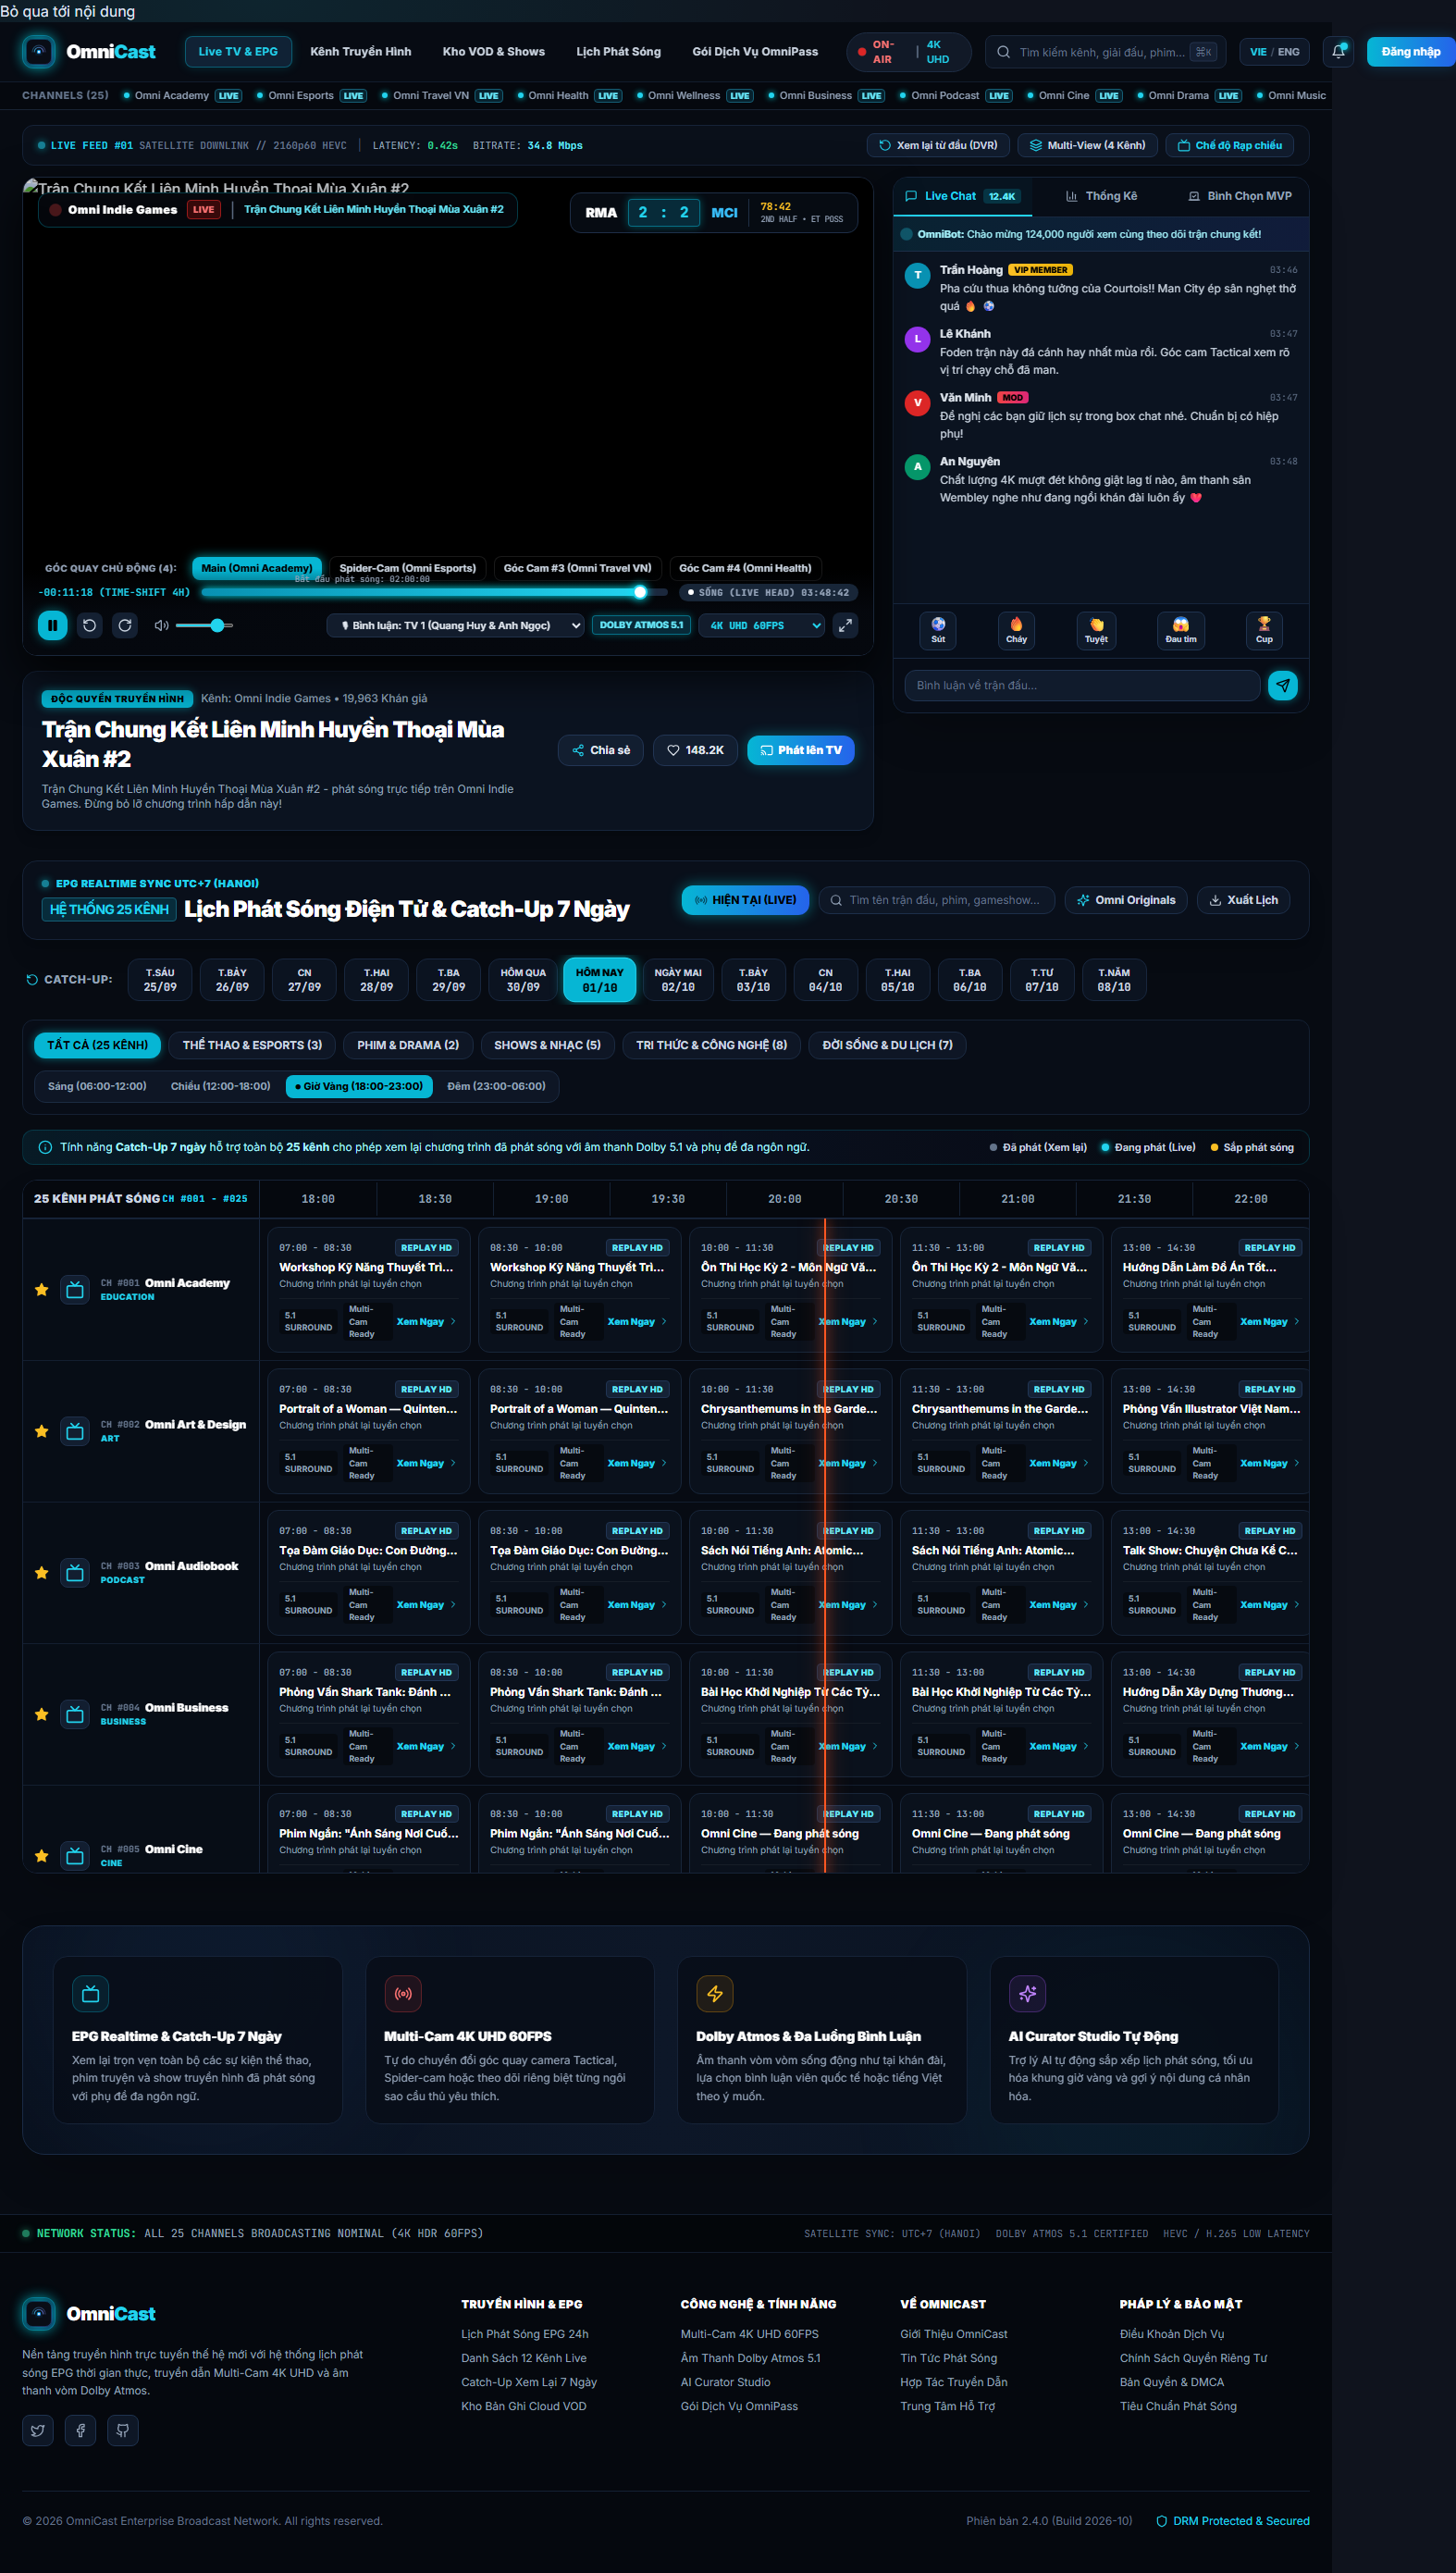
\includegraphics[width=\columnwidth]{../figures/01_home_desktop.png}
\caption{\bi{Trang chủ cổng web trên máy tính: carousel nổi bật, lưới
kênh theo thể loại và thanh điều hướng theo vai trò.}{The web portal
home page on desktop: featured carousel, channel grid by category and
the role-aware navigation bar.}}
\label{fig:home}
\end{figure}

\subsection{\bi{Danh mục đầy đủ 33 Route và Màn hình Web}{Complete 33-Route Web Portal Inventory}}

\bi{
Cổng web cung cấp đầy đủ 33 route được sinh từ 24 thư mục trong \texttt{frontend/app/}.
Bảng~\ref{tab:web_routes} liệt kê toàn bộ 33 màn hình được phân thành năm cụm chức năng:
(1) Nội dung \& Khám phá công khai; (2) Phòng xem LiveStream \& VOD; (3) Bàn điều khiển Live Studio \& Trợ lý AI Curator (\texttt{STAFF}/\texttt{ADMIN}); (4) Tài khoản, Cá nhân hoá \& Quản trị (\texttt{ADMIN}); và (5) Hệ thống Trang Pháp lý \& Tiêu chuẩn Phát sóng.
}{
The web portal exposes 33 routes generated from 24 directories under
\texttt{frontend/app/}. Table~\ref{tab:web_routes} catalogues all 33 screens across five functional clusters:
(1) Public Discovery \& EPG; (2) Interactive LiveStream \& VOD Rooms; (3) Live Studio Console \& AI Curator Suite (\texttt{STAFF}/\texttt{ADMIN}); (4) Account, Personalisation \& Administration (\texttt{ADMIN}); and (5) Legal, Compliance \& Broadcast Standards.
}

\begin{table*}[t]
\caption{\bi{Danh mục toàn bộ 33 Route và Màn hình trên Cổng Web Next.js 15 của OmniCast.}{Complete inventory of all 33 Next.js 15 web portal routes and screens in OmniCast.}}
\label{tab:web_routes}
\centering
\scriptsize
\begin{tabular}{@{}p{2.8cm}p{3.6cm}p{1.6cm}p{8.8cm}@{}}
\toprule
\textbf{\bi{Cụm chức năng}{Cluster}} & \textbf{\bi{Đường dẫn Route (33)}{Route Path (33)}} & \textbf{\bi{Phân quyền}{RBAC Role}} & \textbf{\bi{Tính năng \& Thao tác màn hình chính}{Key Screen Features \& Interactive Operations}} \\
\midrule
\multirow{6}{2.8cm}{\textbf{\bi{1. Khám phá \& Lịch phát EPG}{1. Public Discovery \& EPG}}}
  & \texttt{/}, \texttt{/channels}, \texttt{/channels/[id]} & Public & \bi{Carousel sự kiện tâm điểm, danh mục kênh lọc theo thể loại, trang chi tiết kênh kèm luồng đang phát \& lịch EPG.}{Hero spotlight carousel, category-filtered channel grid, channel detail page with live stream \& EPG.} \\
  & \texttt{/epg} & Public & \bi{Lưới lịch phát điện tử 24/7 không trống, thanh chỉ báo giờ hiện tại (Now-Line), lọc theo ngày và kênh.}{Zero-gap 24/7 EPG timeline grid, real-time Now-Line indicator, date and channel filters.} \\
  & \texttt{/programs}, \texttt{/programs/[id]} & Public & \bi{Thư viện chương trình, trang chi tiết chương trình kèm thẻ sản xuất, lịch phát sắp tới và nút lưu Watchlist.}{Programme directory, programme detail page with production tags, upcoming airings and Watchlist button.} \\
  & \texttt{/recordings}, \texttt{/recordings/[id]} & Public & \bi{Kho video VOD đã phát sóng, trình phát lại đa luồng kèm bình luận và gợi ý nội dung cùng thể loại.}{Published VOD recording library, multi-engine replay player with comments and related VODs.} \\
  & \texttt{/search} & Public & \bi{Tìm kiếm liên thực thể (Kênh, Chương trình, Bản ghi VOD) theo từ khóa và thể loại.}{Cross-entity search (Channels, Programmes, VOD Recordings) with keyword and genre filters.} \\
\midrule
\multirow{3}{2.8cm}{\textbf{\bi{2. Phòng Xem LiveStream}{2. LiveStream Rooms}}}
  & \texttt{/live} & Public & \bi{Trung tâm Đang Phát Sóng (Live Hub): tự động làm mới mỗi 15 giây, hiển thị tổng sự kiện LIVE \& tổng mắt xem (CCU), sắp xếp theo độ nóng hoặc mới nhất.}{Live Hub: auto-refreshes every 15s, displays active LIVE event \& total CCU pills, sorts by trending viewers or newest start time.} \\
  & \texttt{/live/[id]} & Public / Viewer & \bi{Phòng xem LiveStream tương tác: 7 giao diện chủ đề theo thể loại, Sảnh chờ \texttt{JoinLobbyCard}, Chế độ Rạp phim (Cinema Mode), đổi chương trình trong \texttt{lineup}, Chat thời gian thực, 4 nút Biểu cảm hạt nổi 0ms, Thông báo ghim từ Host.}{Interactive LiveStream Room: 7 genre-themed lounges, \texttt{JoinLobbyCard} prompt, Cinema Mode, lineup program switcher, real-time Socket.IO chat, 4 floating emoji reactions, pinned host banner.} \\
\midrule
\multirow{5}{2.8cm}{\textbf{\bi{3. Bàn điều khiển Live Studio \& AI}{3. Live Studio \& AI Curator}}}
  & \texttt{/studio}, \texttt{/studio/live} & \texttt{STAFF}+ & \bi{Bàn điều khiển phát sóng trực tiếp 4 Tab: (1) Chọn VOD có sẵn; (2) Tự ghi hình Camera/Màn hình WHIP WebRTC \& Upload kéo-thả có chữ ký Cloudinary; (3) Kho nội dung công khai; (4) Gửi thông báo ghim \& Dừng sóng.}{4-Tab Live Broadcast Console: (1) Curated VOD Live; (2) Camera/Screen WHIP WebRTC \& Signed Cloudinary Dropzone; (3) Verified Public Catalog; (4) Host Announcement \& Stop Broadcast.} \\
  & \texttt{/studio/curator} & \texttt{STAFF}+ & \bi{Trợ lý biên tập AI (\texttt{gpt-4o} + fallback heuristic): chấm điểm cảm xúc, kiểm duyệt đạo đức phát sóng, gợi ý thẻ và thể loại.}{AI Editorial Workbench (\texttt{gpt-4o} + heuristic fallback): sentiment scoring, broadcast compliance check, auto-tagging.} \\
  & \texttt{/studio/curator/audit}, \texttt{/studio/curator/dashboard} & \texttt{STAFF}+ & \bi{Nhật ký kiểm toán phiên bản prompt (\texttt{promptVersion}), thống kê tỷ lệ duyệt và hiệu năng gọi mô hình.}{Prompt-version provenance audit log (\texttt{promptVersion}), suitability breakdown and latency analytics.} \\
\midrule
\multirow{5}{2.8cm}{\textbf{\bi{4. Tài khoản, Cá nhân \& Quản trị}{4. Account \& Admin}}}
  & \texttt{/login}, \texttt{/register}, \texttt{/forgot-password}, \texttt{/reset-password} & Public & \bi{Đăng nhập JWT + Google OAuth2, đăng ký tài khoản, khôi phục mật khẩu qua mã xác thực.}{JWT + Google OAuth2 sign-in, account registration, tokenised password recovery.} \\
  & \texttt{/profile}, \texttt{/settings}, \texttt{/watchlist}, \texttt{/notifications} & \texttt{VIEWER}+ & \bi{Hồ sơ cá nhân, quản lý gói VIP, danh sách xem sau đồng bộ đa thiết bị, trung tâm thông báo và thu hồi phiên (\texttt{logout-all}).}{User profile, VIP plan management, cross-device watchlist, notification centre and global session revocation (\texttt{logout-all}).} \\
  & \texttt{/admin}, \texttt{/admin/users}, \texttt{/admin/audit-logs} & \texttt{ADMIN} & \bi{Tổng quan hệ thống, quản lý phân quyền người dùng, tra cứu nhật ký kiểm toán gRPC theo hành động/thực thể.}{System telemetry overview, user RBAC management, gRPC audit log explorer by action/entity.} \\
\midrule
\multirow{2}{2.8cm}{\textbf{\bi{5. Pháp lý \& Hỗ trợ}{5. Legal \& Support}}}
  & \texttt{/terms}, \texttt{/privacy}, \texttt{/dmca}, \texttt{/standards}, \texttt{/broadcasting-standards}, \texttt{/help}, \texttt{/docs} & Public & \bi{Điều khoản sử dụng, chính sách bảo mật, bản quyền DMCA, tiêu chuẩn cộng đồng \& phát sóng, trung tâm trợ giúp và tài liệu kỹ thuật.}{Terms of service, privacy policy, DMCA copyright policy, community \& broadcasting standards, help centre and docs.} \\
\bottomrule
\end{tabular}
\end{table*}

\begin{figure}[t]
\centering
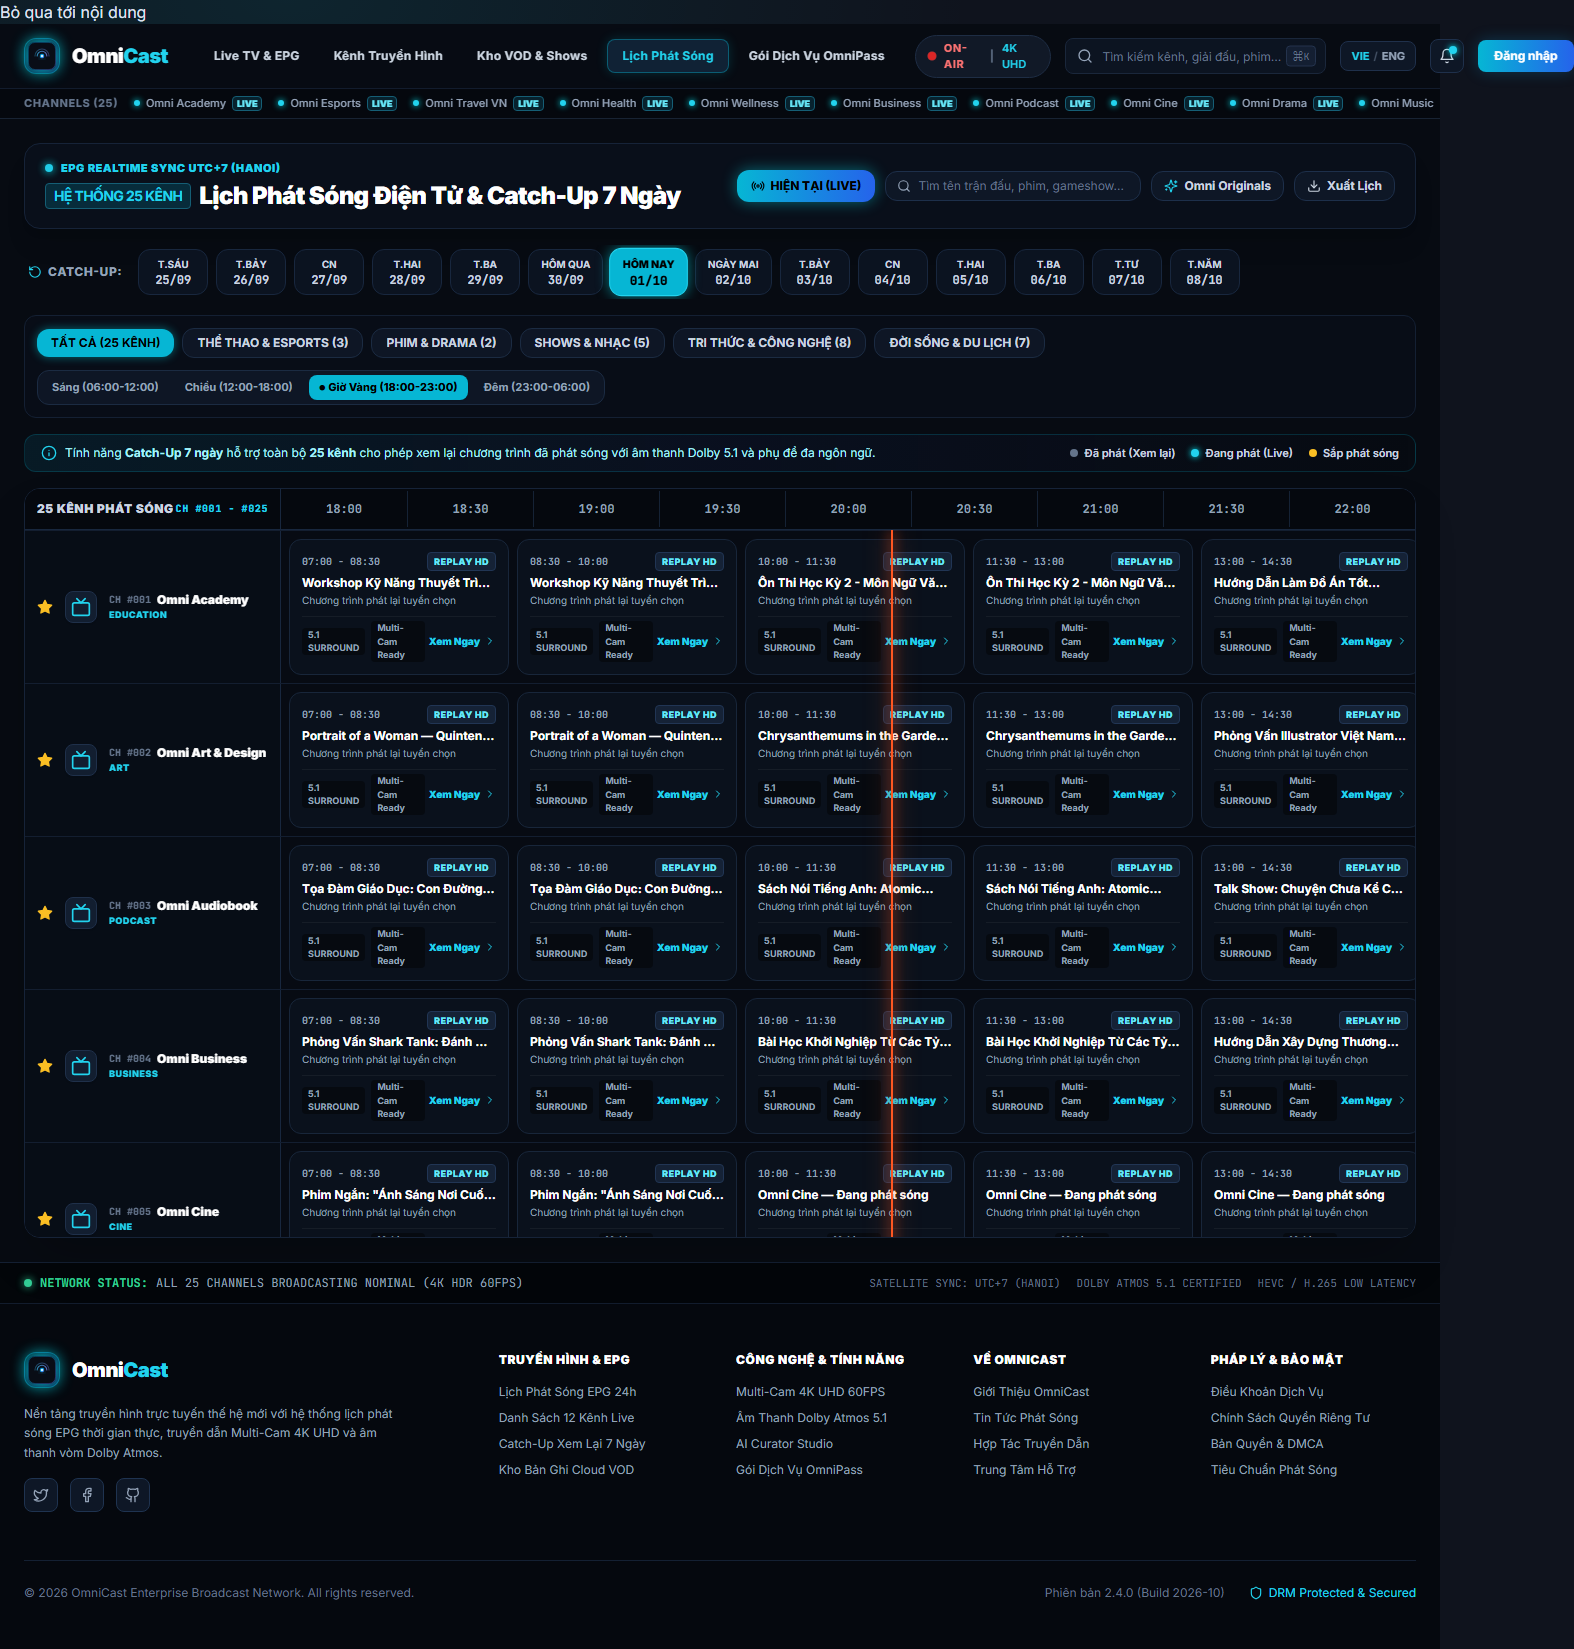
\includegraphics[width=\columnwidth]{../figures/subpage_epg.png}
\caption{\bi{Trang lịch phát điện tử (\texttt{/epg}) với lưới theo khung giờ và bộ chọn
ngày.}{The electronic programme guide page (\texttt{/epg}) with the time-slot grid and
the day selector.}}
\label{fig:epg}
\end{figure}

\subsection{\bi{Màn hình Phòng Xem LiveStream (\texttt{/live} \& \texttt{/live/[id]}) và Các Thao tác Tương tác}{Interactive LiveStream Room (\texttt{/live} \& \texttt{/live/[id]}) and Viewer Operations}}

\bi{
Hệ thống LiveStream trên Web được thiết kế như một không gian truyền hình tương tác toàn diện thông qua hai màn hình cốt lõi:
\begin{enumerate}[leftmargin=*,itemsep=2pt]
  \item \textbf{Trung tâm Phát sóng Trực tiếp (\texttt{/live}):} Tự động đồng bộ danh sách sự kiện đang \texttt{LIVE} mỗi 15 giây, hiển thị hai huy hiệu thống kê thời gian thực ở đầu trang (tổng số sự kiện đang phát và tổng số người đang xem đồng thời), hỗ trợ lọc và sắp xếp theo lượng người xem cao nhất hoặc thời điểm bắt đầu mới nhất, đồng thời hiển thị nút truy cập nhanh vào \texttt{/studio/live} cho người dùng có quyền \texttt{STAFF}/\texttt{ADMIN}.
  \item \textbf{Sảnh chờ Tham gia \& 7 Chủ đề Phòng Live (\texttt{/live/[id]}):} Khi truy cập vào một buổi phát sóng, người xem được chào đón bởi thẻ sảnh chờ \texttt{JoinLobbyCard} hiển thị ảnh thu nhỏ, trạng thái sóng, số mắt xem hiện tại và nút ``Tham gia phòng xem''. Đặc biệt, hàm \texttt{resolveLiveRoomTheme} tự động biến đổi toàn bộ bảng màu nền, viền phát sáng và huy hiệu của phòng xem theo \textbf{7 chủ đề thể loại}: \emph{Kids Wonderland} (Thiếu nhi), \emph{Podcast \& Audiobook} (Ấm áp), \emph{Music Live Stage} (Sân khấu âm nhạc), \emph{Academy \& Tech} (Giáo dục/Khoa học), \emph{Sports Arena} (Đấu trường thể thao), \emph{Obsidian Theater} (Điện ảnh/Phim truyện) và \emph{Broadcast Lounge} (Mặc định).
  \item \textbf{Trình phát Đa luồng, Chế độ Rạp phim (Cinema Mode) \& Chuyển chương trình tức thời:} Trình phát \texttt{VideoPlayer} tự động nhận diện luồng WebRTC/HLS từ MediaMTX (\texttt{cookieCheck=1}), luồng trực tiếp Google Drive hoặc nhúng YouTube. Người xem có thể bật \emph{Chế độ Rạp phim (Cinema Mode)} để làm tối toàn bộ phần tử xung quanh và mở rộng khung hình lên 12 cột. Nếu sự kiện có danh sách phát nhiều phần (\texttt{lineup}) hoặc người dùng là \texttt{STAFF}/\texttt{ADMIN}, thanh chọn chương trình cho phép chuyển đổi video đang phát ngay lập tức cho toàn bộ phòng qua API \texttt{switchProgramOnLiveEvent} mà không cần tải lại trang.
  \item \textbf{Thao tác Tương tác Thời gian thực qua Socket.IO (\texttt{/live}):} Khung tương tác bên phải kết nối trực tiếp tới namespace \texttt{/live}, cho phép khán giả: (i) gửi bình luận trực tiếp có kiểm tra đăng nhập và tự động cuộn mượt; (ii) thả 4 loại biểu cảm nổi (\texttt{HEART} $\heartsuit$, \texttt{FIRE}, \texttt{CLAP}, \texttt{WOW}) bay lên trên khung hình video kèm bộ đếm cộng dồn tức thời; và (iii) nhận thông báo ghim (\texttt{broadcaster:message}) từ đạo diễn hiển thị nổi bật dưới dạng dải băng thông báo ở đầu màn hình.
\end{enumerate}
}{
The web LiveStream experience is engineered as a full-featured interactive broadcast lounge across two core screens:
\begin{enumerate}[leftmargin=*,itemsep=2pt]
  \item \textbf{Live Broadcast Hub (\texttt{/live}):} Polls active \texttt{LIVE} events every 15 seconds, displays real-time header badges for total active broadcasts and aggregate concurrent viewers (CCU), supports sorting by viewer count or start time, and surfaces a direct ``Go to Live Studio'' shortcut for \texttt{STAFF}/\texttt{ADMIN} users.
  \item \textbf{Interactive Lobby \& 7 Genre-Themed Broadcast Lounges (\texttt{/live/[id]}):} Upon entering a stream, viewers encounter a \texttt{JoinLobbyCard} previewing the stream status and live viewer count before entering the room. Once inside, \texttt{resolveLiveRoomTheme} dynamically styles the entire room into one of \textbf{7 genre-specific themes}: \emph{Kids Wonderland}, \emph{Podcast \& Audiobook}, \emph{Music Live Stage}, \emph{Academy \& Tech}, \emph{Sports Arena}, \emph{Obsidian Theater} (Cinema/Drama) and \emph{Broadcast Lounge} (Default).
  \item \textbf{Multi-Engine Player, Cinema Mode \& Instant Lineup Switching:} \texttt{VideoPlayer} seamlessly handles MediaMTX HLS/WebRTC streams (\texttt{cookieCheck=1}), direct Google Drive streams and YouTube embeds. Viewers can toggle \emph{Cinema Mode} (lights-off focus) to dim surrounding chrome and expand the stage to full width. When a broadcast contains multiple lineup items or is controlled by \texttt{STAFF}/\texttt{ADMIN}, the lineup bar triggers \texttt{switchProgramOnLiveEvent}, switching the active video stream for all viewers in the room without page reload.
  \item \textbf{Real-Time Socket.IO (\texttt{/live}) Operations:} The live interaction sidebar connects to the \texttt{/live} namespace, enabling viewers to: (i) post real-time chat messages with auto-scroll; (ii) fire 4 floating emoji reactions (\texttt{HEART}, \texttt{FIRE}, \texttt{CLAP}, \texttt{WOW}) that animate upward over the video canvas with optimistic counter updates; and (iii) receive pinned host announcements (\texttt{broadcaster:message}) rendered as a prominent banner across the stage.
\end{enumerate}
}

\subsection{\bi{Màn hình Bàn điều khiển Web Live Studio (\texttt{/studio/live})}{Web Live Studio Broadcast Console (\texttt{/studio/live})}}

\bi{
Trang \texttt{/studio/live} (\texttt{frontend/app/studio/live/page.tsx}) cung cấp bàn điều khiển phát sóng chuyên nghiệp dành cho \texttt{STAFF} và \texttt{ADMIN} với 4 chế độ vận hành:
\begin{itemize}[leftmargin=*,itemsep=1pt]
  \item \textbf{Tab 1 --- Chọn nội dung phát sóng (Curated Live):} Chọn kênh đích, nhập tiêu đề/mô tả phiên Live, tìm kiếm và chọn một hoặc nhiều bản ghi từ thư viện kênh hoặc kho chung để phát sóng liên tiếp (\texttt{lineup}).
  \item \textbf{Tab 2 --- Tự ghi hình / Tải tệp / Phát trực tiếp từ Camera (\texttt{WebcamLiveBroadcaster} \& \texttt{WebStudioViewfinder}):} Hỗ trợ quay trực tiếp từ Camera máy tính, chia sẻ màn hình (\texttt{getDisplayMedia}), phát trực tiếp độ trễ thấp qua giao thức WebRTC WHIP tới MediaMTX, hoặc kéo-thả tệp video vào \texttt{UploadDropzone} + \texttt{UploadQueue} (tải lên trực tiếp Cloudinary bằng chữ ký số, hiển thị thanh tiến trình, tốc độ MB/s, thời gian còn lại ETA, tự động trích xuất ảnh thu nhỏ bằng \texttt{canvas} và hỗ trợ 3 chế độ xuất bản: Phát ngay \texttt{IMMEDIATE}, Hẹn lịch \texttt{SCHEDULED} hoặc Lưu nháp \texttt{PRIVATE}).
  \item \textbf{Tab 3 --- Kho nội dung công khai (Verified Public Catalog):} Duyệt danh sách các luồng HLS/MP4 công khai đã kiểm định, lọc theo định dạng và nhập một chạm vào thư viện kênh.
  \item \textbf{Tab 4 --- Điều hành \& Tương tác trực tiếp:} Cho phép đạo diễn gửi thông báo ghim (\texttt{broadcaster:message}) tới mọi người xem trong phòng và kết thúc phiên phát sóng (\texttt{stopLiveEvent}) kèm tùy chọn giữ lại bản ghi làm VOD.
\end{itemize}
}{
The \texttt{/studio/live} route (\texttt{frontend/app/studio/live/page.tsx}) provides a production-grade broadcast control console for \texttt{STAFF} and \texttt{ADMIN} operators across four tabs:
\begin{itemize}[leftmargin=*,itemsep=1pt]
  \item \textbf{Tab 1 --- Curated Live:} Select the target channel, configure broadcast metadata, and pick one or more VOD recordings from the channel or global library to launch a multi-item \texttt{lineup}.
  \item \textbf{Tab 2 --- Self-Record / File Upload / Webcam WHIP Live (\texttt{WebcamLiveBroadcaster} \& \texttt{WebStudioViewfinder}):} Supports browser camera capture, screen sharing (\texttt{getDisplayMedia}), direct WebRTC WHIP publishing to MediaMTX, or drag-and-drop file ingestion via \texttt{UploadDropzone} + \texttt{UploadQueue} (signed direct-to-Cloudinary upload with live MB/s speed, ETA, automatic HTML5 \texttt{canvas} thumbnail extraction, and 3 visibility modes: \texttt{IMMEDIATE}, \texttt{SCHEDULED}, \texttt{PRIVATE}).
  \item \textbf{Tab 3 --- Verified Public Catalog:} Browse verified HLS/MP4 streams with format filters and one-click channel library import.
  \item \textbf{Tab 4 --- Live Host Console:} Send pinned broadcaster announcements (\texttt{broadcaster:message}) to all connected viewers and terminate active broadcasts (\texttt{stopLiveEvent}) with the \texttt{keepAsVod} archival option.
\end{itemize}
}

\subsection{\bi{Giao diện theo vai trò và Trợ lý AI Curator}{Role-Aware Interface and AI Curator Suite}}

\bi{
Một tệp cấu hình duy nhất, \texttt{frontend/lib/constants/role-config.ts},
quyết định thành phần nào xuất hiện cho từng vai trò. Hàm
\texttt{hasMinimumRole} so sánh thứ hạng vai trò, nên việc nâng một
quyền từ \texttt{VIEWER} lên \texttt{STAFF} chỉ là sửa một dòng.
Trang \texttt{/studio/curator} là giao diện biên tập AI: hiển thị danh
sách chương trình chờ duyệt, cho phép chạy lại quy trình AI, xem
điểm tin cậy, phân loại phù hợp phát sóng và các cảnh báo tuân thủ.
Trang \texttt{/studio/curator/audit} trình bày lịch sử các lần chạy
AI với dấu vết phiên bản prompt, và \texttt{/studio/curator/dashboard} tổng hợp thống kê
phân bố theo thể loại và mức độ phù hợp phát sóng.
}{
A single configuration file,
\texttt{frontend/lib/constants/role-config.ts}, determines which
components appear for each role. The \texttt{hasMinimumRole} helper
compares role ranks, so promoting a capability from \texttt{VIEWER} to
\texttt{STAFF} is a one-line edit. The \texttt{/studio/curator} page is the AI curation interface: it
lists programmes awaiting review, allows re-running the AI pipeline,
and exposes the confidence score, broadcast-suitability classification
and compliance flags. The \texttt{/studio/curator/audit} page presents
the run history with prompt-version provenance, while \texttt{/studio/curator/dashboard}
aggregates statistics by category and broadcast suitability.
}

\begin{figure}[t]
\centering
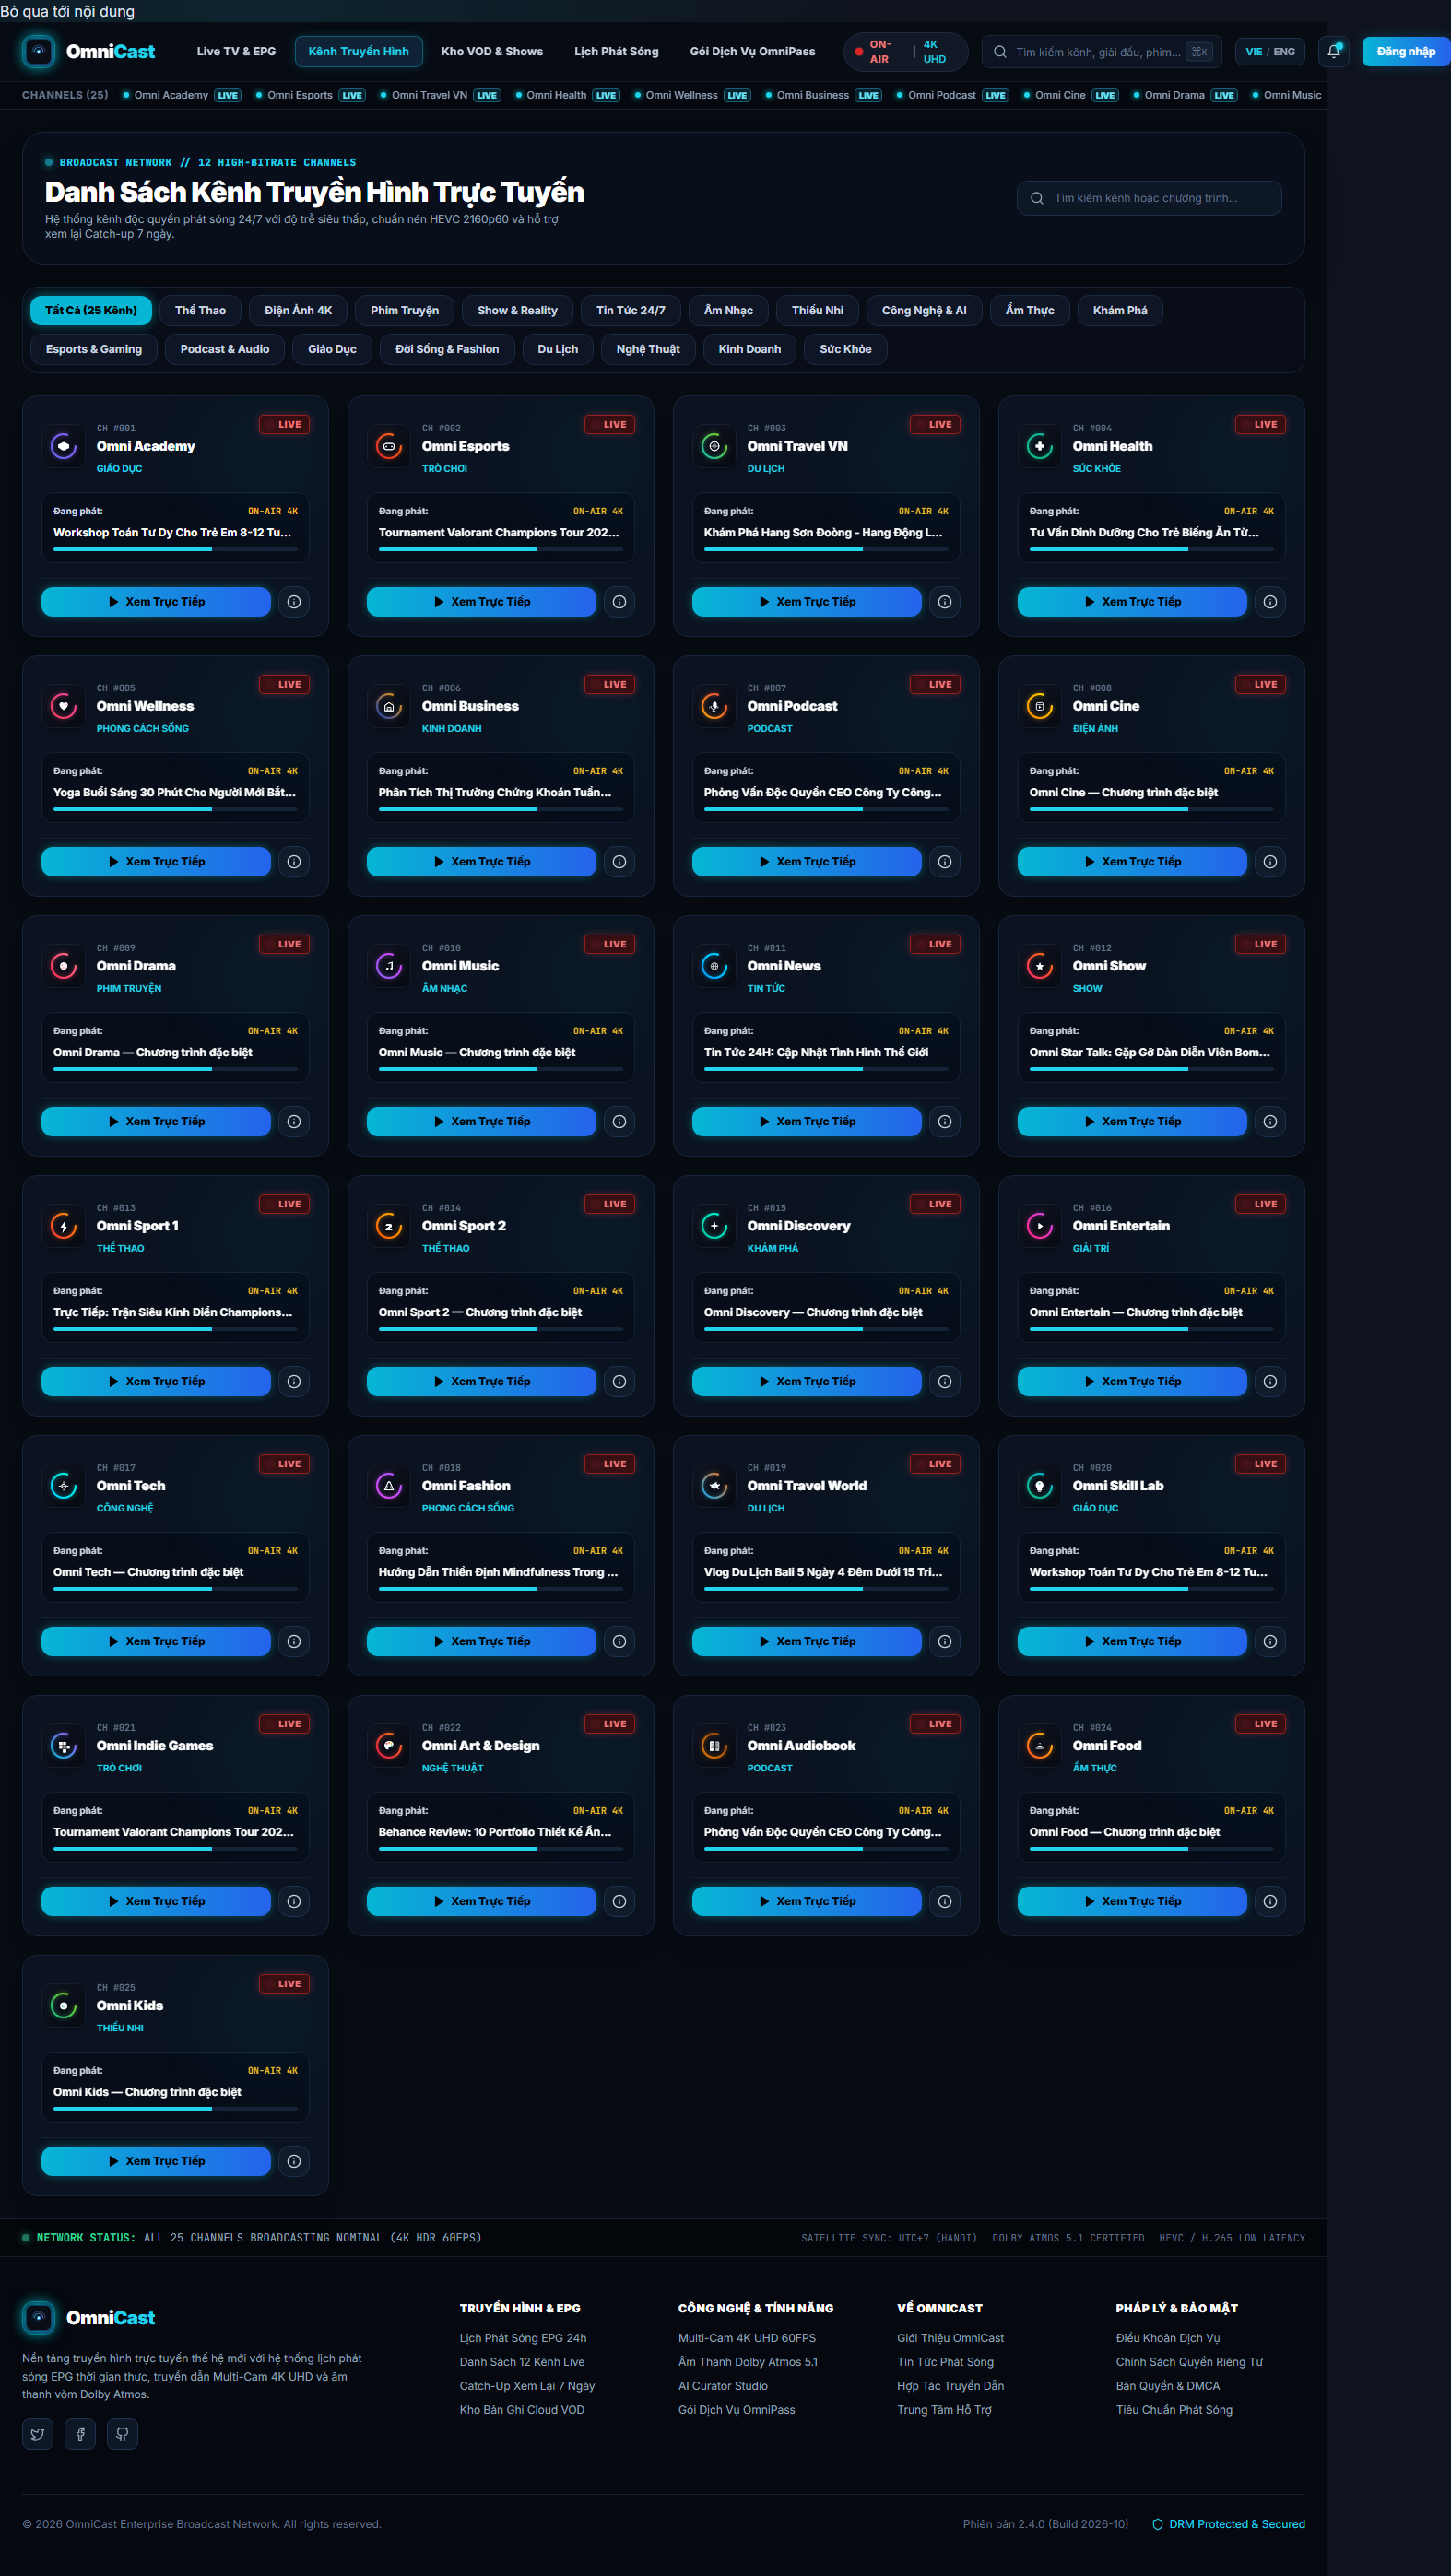
\includegraphics[width=\columnwidth]{../figures/subpage_channels.png}
\caption{\bi{Trang danh mục kênh (\texttt{/channels}) với bộ lọc theo thể loại và thẻ nội
dung.}{The channel catalogue page (\texttt{/channels}) with category filters and content
badges.}}
\label{fig:channels}
\end{figure}

\subsection{\bi{Bảo mật phía client, Quản lý phiên và Kiểm thử}{Client-Side Security, Session Handling and Testing}}

\bi{
Cổng web dùng \texttt{next-themes} để hỗ trợ chế độ sáng/tối và một
lớp \texttt{safe-log} (\texttt{redact.ts}) loại bỏ mọi dữ liệu nhạy cảm (mật khẩu, token, khóa API) trước khi ghi log. Khi người dùng đăng xuất, mọi phiên đăng nhập trên thiết bị khác được
thu hồi qua endpoint \texttt{logout-all}.
Cổng web có 228 kiểm thử Vitest trong 76 bộ kiểm thử, bao phủ các hàm
thuần (\texttt{query-builder}, \texttt{curator-filters},
\texttt{curator-helpers}, \texttt{redact}, \texttt{safe-log},
\texttt{utils}), các hook (\texttt{useAiCurator},
\texttt{useAiCuratorStats}), các hàm cấu hình (\texttt{role-config}) và
các thành phần React (\texttt{video-player},
\texttt{save-to-watchlist}, các trang pháp lý, các trang studio).
CI còn chạy \texttt{tsc --noEmit} để bắt lỗi kiểu dữ liệu trước khi
biên dịch.
}{
The portal uses \texttt{next-themes} for light/dark support and a
\texttt{safe-log} layer (\texttt{redact.ts}) that masks sensitive fields (passwords, tokens, API keys) before logging. On
logout, sessions on other devices are revoked through the
\texttt{logout-all} endpoint.
The portal carries 228 Vitest tests across 76 suites, covering pure
functions (\texttt{query-builder}, \texttt{curator-filters},
\texttt{curator-helpers}, \texttt{redact}, \texttt{safe-log},
\texttt{utils}), hooks (\texttt{useAiCurator},
\texttt{useAiCuratorStats}), configuration (\texttt{role-config}) and
React components (\texttt{video-player}, \texttt{save-to-watchlist},
the legal pages, the studio pages). CI additionally runs
\texttt{tsc --noEmit} to catch type errors before the build.
}

% ============================================================
% PRN232 - Section 6: Database Design (Vietnamese & English)
% ============================================================
\section{\bi{Thiết kế cơ sở dữ liệu}{Database Design}}
\label{sec:db}

\subsection{\bi{Cơ sở dữ liệu quan hệ với Prisma}{Relational Database with Prisma}}

\bi{
Toàn bộ dữ liệu nghiệp vụ nằm trong PostgreSQL, được định nghĩa bằng
21 model Prisma trong \texttt{backend/prisma/schema.prisma}. Prisma
đóng vai trò lớp trừu tượng hoá: mọi truy vấn được viết bằng API
có kiểu \texttt{findMany}, \texttt{upsert} hoặc \texttt{createMany} và
được biên dịch thành SQL tham số hoá, nhờ vậy loại bỏ hoàn toàn khả
năng chèn SQL trực tiếp từ mã ứng dụng. Hình~\ref{fig:db_arch} minh hoạ sơ đồ kiến trúc 5 miền dữ liệu của 21 model Prisma.
}{
All business data resides in PostgreSQL, defined by 21 Prisma models in
\texttt{backend/prisma/schema.prisma}. Prisma acts as the
abstraction layer: every query is written against a typed API such as
\texttt{findMany}, \texttt{upsert} or \texttt{createMany} and compiled
into parameterised SQL, which eliminates the possibility of injecting
raw SQL from application code. Fig.~\ref{fig:db_arch} illustrates the 5-domain relational architecture across all 21 Prisma models.
}

\begin{figure*}[t]
\centering
\fitfull{\figDatabaseArchitecture}
\caption{\bi{Sơ đồ kiến trúc cơ sở dữ liệu quan hệ 5 miền nghiệp vụ (21 model Prisma trên Supabase PostgreSQL).}{Five-domain relational database architecture diagram (21 Prisma models on Supabase PostgreSQL).}}
\label{fig:db_arch}
\end{figure*}

\begin{table}[t]
\caption{\bi{21 model Prisma cùng số trường vô hướng và quan hệ.}{The 21
Prisma models with their scalar and relation field counts.}}
\label{tab:erd}
\centering
\scriptsize
\fitcol{% Auto-generated from backend/prisma/schema.prisma - do not edit by hand.
\begin{tabular}{@{}llrr@{}}
\toprule
\textbf{\bi{Model}{Model}} & \textbf{\bi{Vai trò nghiệp vụ}{Business role}} & \textbf{\bi{Scalar}{Scalar}} & \textbf{\bi{Quan hệ}{Relation}} \\
\midrule
\texttt{User} & \bi{Tài khoản người dùng + RBAC}{User account + RBAC} & 14 & 13 \\
\texttt{RefreshToken} & \bi{Xoay vòng phiên đăng nhập}{Rotating login sessions} & 6 & 1 \\
\texttt{PasswordResetToken} & \bi{Đặt lại mật khẩu (TTL 1h)}{Password reset (1h TTL)} & 7 & 1 \\
\texttt{ProductionTag} & \bi{Thẻ nội dung theo chương trình}{Content tag per production} & 5 & 0 \\
\texttt{LiveChannel} & \bi{Kênh phát sóng trực tiếp}{Broadcast channel} & 29 & 5 \\
\texttt{LiveEvent} & \bi{Sự kiện phát sóng / chương trình}{Live event / programme} & 32 & 7 \\
\texttt{Recording} & \bi{Bản ghi đã phát}{Published recording} & 42 & 5 \\
\texttt{Podcast} & \bi{Chuyên mục podcast}{Podcast collection} & 12 & 3 \\
\texttt{PodcastEpisode} & \bi{Tập podcast}{Podcast episode} & 12 & 1 \\
\texttt{Follow} & \bi{Theo dõi kênh}{Channel follow} & 4 & 2 \\
\texttt{Comment} & \bi{Bình luận}{Comment} & 11 & 6 \\
\texttt{CommentLike} & \bi{Like bình luận}{Comment like} & 4 & 2 \\
\texttt{Reaction} & \bi{Cảm xúc realtime}{Realtime reaction} & 6 & 3 \\
\texttt{WatchHistory} & \bi{Lịch sử xem}{Watch history} & 8 & 2 \\
\texttt{Notification} & \bi{Thông báo trong ứng dụng}{In-app notification} & 13 & 2 \\
\texttt{AuditLog} & \bi{Nhật ký kiểm toán (gRPC)}{Audit log (gRPC)} & 11 & 0 \\
\texttt{Watchlist} & \bi{Danh sách theo dõi}{Watchlist} & 7 & 1 \\
\texttt{AiCuratorReport} & \bi{Báo cáo AI Curator}{AI Curator report} & 15 & 1 \\
\texttt{DeviceToken} & \bi{Token thiết bị FCM}{FCM device token} & 8 & 1 \\
\texttt{NewsletterSubscriber} & \bi{Người đăng ký newsletter}{Newsletter subscriber} & 14 & 1 \\
\texttt{StreamDonation} & \bi{Quyên góp trong livestream}{Livestream donation} & 14 & 3 \\
\bottomrule
\end{tabular}
}
\end{table}

\subsection{\bi{Phân nhóm miền dữ liệu}{Data-Domain Grouping}}

\bi{
Các model được tổ chức theo năm nhóm nghiệp vụ:
}{
The models are organised into five business groups:
}

\begin{itemize}[leftmargin=*,itemsep=1pt]
  \item \bi{\textbf{Xác thực và danh tính.} \texttt{User} lưu thông tin
  tài khoản cùng vai trò, \texttt{RefreshToken} lưu phiên đăng nhập
  xoay vòng, \texttt{PasswordResetToken} lưu mã đặt lại mật khẩu với
  thời hạn một giờ.}{
  \textbf{Authentication and identity.} \texttt{User} stores account
  details together with the role, \texttt{RefreshToken} stores
  rotating login sessions, and \texttt{PasswordResetToken} stores
  password-reset codes with a one-hour lifetime.}

  \item \bi{\textbf{Nội dung phát sóng.} \texttt{LiveChannel} là kênh,
  \texttt{LiveEvent} là chương trình trong lịch và phiên phát sóng trực tiếp, \texttt{Recording}
  là bản ghi đã phát, \texttt{ProductionTag} là thẻ nội dung gắn với
  chương trình.}{
  \textbf{Broadcast content.} \texttt{LiveChannel} is the channel,
  \texttt{LiveEvent} is a scheduled programme and active live broadcast, \texttt{Recording} is
  a published recording and \texttt{ProductionTag} is a content tag
  attached to a production.}

  \item \bi{\textbf{Tương tác người dùng \& Thương mại Live.} \texttt{Comment},
  \texttt{CommentLike}, \texttt{Reaction}, \texttt{Follow},
  \texttt{WatchHistory}, \texttt{Watchlist} và
  \texttt{StreamDonation} (quyên góp Super Chat trong phòng Live) mô tả toàn bộ hành vi của người xem.}{
  \textbf{User interaction \& Live Monetization.} \texttt{Comment}, \texttt{CommentLike},
  \texttt{Reaction}, \texttt{Follow}, \texttt{WatchHistory},
  \texttt{Watchlist} and \texttt{StreamDonation} (Super Chat live donations) describe the full
  spectrum of viewer behaviour.}

  \item \bi{\textbf{Vận hành và kiểm toán.} \texttt{AuditLog} nhận
  bản ghi từ microservice gRPC, \texttt{Notification} lưu thông báo
  trong ứng dụng, \texttt{DeviceToken} lưu token FCM,
  \texttt{NewsletterSubscriber} lưu người đăng ký bản tin.}{
  \textbf{Operations and auditing.} \texttt{AuditLog} receives records
  from the gRPC microservice, \texttt{Notification} stores in-app
  notifications, \texttt{DeviceToken} stores FCM tokens and
  \texttt{NewsletterSubscriber} stores newsletter subscribers.}

  \item \bi{\textbf{Trợ lý AI.} \texttt{AiCuratorReport} lưu kết quả
  biên tập AI kèm dấu vết phiên bản prompt và mô hình.}{
  \textbf{AI assistance.} \texttt{AiCuratorReport} stores AI curation
  output together with its prompt and model version provenance.}
\end{itemize}

\subsection{\bi{Quan hệ và ràng buộc}{Relationships and Constraints}}

\bi{
Quan hệ được định nghĩa bằng khóa ngoại chuẩn của Prisma, và mỗi quan
hệ đều có chỉ mục phù hợp với truy vấn hot-path. Ba ràng buộc đáng
chú ý:
}{
Relationships are expressed with standard Prisma foreign keys, and
each carries an index matched to its hot-path query. Three constraints
deserve attention:
}

\begin{enumerate}[leftmargin=*,itemsep=1pt]
  \item \bi{\textbf{Xoá người dùng không phá vỡ nhật ký kiểm toán.}
  \texttt{RefreshToken.user} có quan hệ \texttt{OnDelete: SetNull},
  nên xoá tài khoản chỉ vô hiệu hoá phiên mà vẫn giữ được dấu vết
  kiểm toán.}{
  \textbf{User deletion does not destroy the audit trail.}
  \texttt{RefreshToken.user} uses \texttt{OnDelete: SetNull}, so
  deleting an account invalidates the sessions while preserving the
  audit trail.}

  \item \bi{\textbf{Khoá duy nhất trên thẻ nội dung.} \texttt{ProductionTag}
  có khoá duy nhất trên cặp chương trình và tên thẻ, nên cùng một thẻ
  không thể bị gán hai lần.}{
  \textbf{A unique key on content tags.} \texttt{ProductionTag} carries
  a unique constraint on the programme-and-tag pair, so the same tag
  cannot be attached twice.}

  \item \bi{\textbf{Chỉ mục theo trục thời gian.} Các truy vấn EPG
  luôn lọc theo \texttt{scheduledAt} và \texttt{channelId}, nên cột
  này được chỉ mục; truy vấn lịch sử xem lọc theo
  \texttt{userId} và \texttt{watchedAt}.}{
  \textbf{Time-axis indexes.} EPG queries always filter by
  \texttt{scheduledAt} and \texttt{channelId}, so those columns are
  indexed; watch-history queries filter by \texttt{userId} and
  \texttt{watchedAt}.}
\end{enumerate}

\subsection{\bi{Chuẩn hoá và quyết định thiết kế}{Normalisation and Design Decisions}}

\bi{
Mô hình được chuẩn hoá ở mức 3NF: các thuộc tính chỉ phụ thuộc khóa
chính, không có phụ thuộc hàm bắc cầu giữa các thuộc tính
không khóa. Hai quyết định thiết kế đáng bàn:
}{
The model is normalised to third normal form: attributes depend only on
the primary key and no non-key attribute depends transitively on
another. Two design decisions deserve discussion:
}

\begin{itemize}[leftmargin=*,itemsep=1pt]
  \item \bi{\textbf{Chuẩn hoá cấu trúc EPG.} Thay vì lưu lưới 24
  giờ đã điền, hệ thống lưu các sự kiện thật cùng thẻ nội dung, và
  lưới được tính lại khi truy vấn. Cách này giữ dữ liệu gốc trung
  thực và cho phép lịch thay đổi mà không cần di chuyển dữ liệu, đổi
  lại tốn công tính toán tại thời điểm đọc --- một đánh đổi đúng đắn
  khi phần lớn thao tác ghi là chương trình biên tập và phần lớn
  thao tác đọc là xem lịch.}{
  \textbf{EPG structure normalisation.} Rather than storing the
  filled 24-hour grid, the system stores real events with content tags
  and recomputes the grid on demand. This keeps the source data
  truthful and lets schedules change without data migration, at the
  cost of computation at read time --- a sound trade-off when most
  writes are editorial and most reads are schedule viewing.}

  \item \bi{\textbf{Không lưu sẵn báo cáo AI trong JSON blob.}
  \texttt{AiCuratorReport} có các cột riêng cho từng trường quan
  trọng (điểm tin cậy, phân loại phù hợp phát sóng, cờ tuân thủ)
  để có thể lọc và thống kê bằng SQL, chỉ giữ phần phân tích tự do
  dạng văn bản trong trường riêng.}{
  \textbf{AI reports are not stored as a JSON blob.}
  \texttt{AiCuratorReport} exposes separate columns for each important
  field (confidence score, broadcast-suitability class, compliance
  flags) so they can be filtered and aggregated in SQL, keeping only
  the free-form analysis in a dedicated text column.}
\end{itemize}

\subsection{\bi{Quản lý phiên bản lược đồ}{Schema Versioning}}

\bi{
Mọi thay đổi lược đồ đều được quản lý bằng \texttt{prisma migrate},
tạo ra các tệp SQL trong \texttt{backend/prisma/migrations} được đưa
vào kiểm soát phiên bản. CI chạy \texttt{prisma migrate deploy} trên
một dịch vụ PostgreSQL 15 tạm trước khi biên dịch ứng dụng, nhờ vậy
một lược đồ không tương thích sẽ bị phát hiện trước khi triển khai
sản xuất.
}{
Every schema change is managed through \texttt{prisma migrate}, which
generates SQL files under \texttt{backend/prisma/migrations} that are
kept under version control. CI runs \texttt{prisma migrate deploy}
against a temporary PostgreSQL 15 service before building the
application, so an incompatible schema is detected before any
production deployment.
}

% ============================================================
% PRN232 - Section 7: Testing (Vietnamese)
% ============================================================
\section{\bi{Kiểm thử và đánh giá}{Testing and Evaluation}}
\label{sec:test}

\subsection{\bi{Chiến lược kiểm thử}{Test Strategy}}

\bi{
Dự án áp dụng chiến lược kiểm thử theo tầng, trong đó trọng tâm là
kiểm thử đơn vị cho logic nghiệp vụ vì đây là phần chứa nhiều quy tắc
tinh vi nhất. Điểm đặc biệt của dự án là \emph{toàn bộ bộ kiểm thử
back-end chạy được mà không cần cơ sở dữ liệu}: mỗi spec file tiêm
một đối tượng Prisma giả (fake client), nhờ vậy chu kỳ kiểm thử rất
ngắn và hoàn toàn xác định.
}{
The project applies a layered test strategy, with unit testing of the
business rules taking priority because that layer holds the most
subtle logic. A distinctive property of this project is that the
\emph{entire back-end suite runs without a database}: each spec file
injects a fake Prisma client, so the test cycle is short and fully
deterministic.
}

\subsection{\bi{Kết quả thực thi}{Execution Results}}

\bi{
Các bộ kiểm thử được chạy thật trên máy dự án ngày 28 tháng 10 năm
2026. Toàn bộ 482 kiểm thử đều đạt, không có kiểm thử nào bị bỏ qua
hoặc lỗi.
}{
All suites were executed on the project machine on 28 October 2026.
All 482 tests pass, with no skipped or errored test.
}

\begin{table}[t]
\caption{\bi{Kết quả kiểm thử tự động của ba bộ kiểm thử.}{Automated
test results across the three suites.}}
\label{tab:tests}
\centering
\footnotesize
\fitcol{% Auto-generated from deliverables/02_Testing/test-results - do not edit by hand.
\begin{tabular}{@{}llrr@{}}
\toprule
\textbf{\bi{Bộ kiểm thử}{Test suite}} & \textbf{\bi{Lệnh chạy}{Command}} & \textbf{\bi{Tổng}{Total}} & \textbf{\bi{Đạt}{Passed}} \\
\midrule
\bi{Backend (node:test)}{Backend (node:test)} & \texttt{npm test} & 163 & 163 \\
\bi{Frontend (Vitest)}{Frontend (Vitest)} & \texttt{npx vitest run} & 228 & 228 \\
\bi{Mobile (flutter test)}{Mobile (flutter test)} & \texttt{flutter test} & 91 & 91 \\
\midrule
\textbf{\bi{Tổng cộng}{Total}} & & \textbf{482} & \textbf{482} \\
\bottomrule
\end{tabular}
}
\end{table}

\subsection{\bi{Bộ kiểm thử back-end}{Back-End Test Suite}}

\bi{
Bộ kiểm thử back-end dùng trình chạy \texttt{node:test} tích hợp sẵn
của Node.js 20, đi kèm một runner tự viết
(\texttt{backend/test/runner.js}) biên dịch các spec bằng
\texttt{tsc} rồi thực thi tuần tự. Việc chọn trình chạy tích hợp
thay vì Jest hay Vitest giúp loại bỏ hoàn toàn phụ thuộc bên thứ ba
trong bộ kiểm thử, giảm bề mặt lỗi và giữ cho quy trình CI ổn định.
}{
The back-end suite uses Node.js 20's built-in \texttt{node:test}
runner together with a custom runner (\texttt{backend/test/runner.js})
that compiles the specs with \texttt{tsc} and executes them
sequentially. Choosing the built-in runner over Jest or Vitest removes
every third-party dependency from the test path, shrinking the failure
surface and keeping the CI pipeline stable.
}

\begin{table}[t]
\caption{\bi{Phân bố kiểm thử back-end theo tệp spec.}{Back-end test
distribution per spec file.}}
\label{tab:backend-specs}
\centering
\scriptsize
\begin{tabular}{@{}lrl@{}}
\toprule
\textbf{Tệp spec} & \textbf{\bi{Kiểm thử đạt}{Tests passed}} & \textbf{\bi{Tỉ lệ đạt}{Pass rate}} \\
\midrule
\texttt{ai-curator.service.spec.ts}       & 19 & 100\% \\
\texttt{epg-filler.spec.ts}               & 18 & 100\% \\
\texttt{live-studio.service.spec.ts}      & 18 & 100\% \\
\texttt{auth.service.spec.ts}             & 17 & 100\% \\
\texttt{ai-curator.e2e.spec.ts}           & 13 & 100\% \\
\texttt{watchlist.service.spec.ts}        & 11 & 100\% \\
\texttt{ingest-sources.spec.ts}           & 11 & 100\% \\
\texttt{ai-curator-stats.service.spec.ts} & 10 & 100\% \\
\texttt{channels.service.spec.ts}         &  7 & 100\% \\
\texttt{programs.conflict.spec.ts}        &  7 & 100\% \\
\texttt{programs.counter.spec.ts}         &  8 & 100\% \\
\texttt{audit-logger.service.spec.ts}     &  8 & 100\% \\
\texttt{epg-timeline.spec.ts}             &  5 & 100\% \\
\texttt{search.service.spec.ts}           &  4 & 100\% \\
\texttt{users.service.spec.ts}            &  4 & 100\% \\
\texttt{billing.service.spec.ts}          &  3 & 100\% \\
\midrule
\textbf{Tổng} & \textbf{163} & \textbf{100\%} \\
\bottomrule
\end{tabular}
\end{table}

\bi{
Hai tệp kiểm thử đáng chú ý nhất vì chúng bảo vệ trực tiếp các thuật
toán nghiệp vụ cốt lõi. \texttt{programs.conflict.spec.ts} kiểm tra
thuật toán phát hiện xung đột trên cả ba dạng giao thoa, trường hợp
giá trị thời lượng bằng \texttt{NULL}, và trường hợp loại trừ chính
sự kiện đang cập nhật. \texttt{epg-filler.spec.ts} kiểm tra tính
đầy đủ 24 giờ của lưới, tính xác định của lựa chọn ngẫu nhiên có
hạt giống, giới hạn số lần phát lại, và hành vi tách tập.
}{
Two spec files deserve particular mention because they directly
protect the core algorithms. \texttt{programs.conflict.spec.ts}
exercises the conflict detector across all three overlap forms, the
\texttt{NULL}-duration case and the self-exclusion case used when
updating an event. \texttt{epg-filler.spec.ts} verifies the
completeness of the 24-hour grid, the determinism of the seeded
selection, the repeat limit and the episode-splitting behaviour.
}

\subsection{\bi{Bộ kiểm thử web}{Web Test Suite}}

\bi{
228 kiểm thử Vitest trong 76 bộ kiểm thử bao phủ cả ba loại đối
tượng: hàm thuần, hook React và thành phần giao diện. Các hàm thuần
được kiểm thử với đầy đủ trường hợp biên (chuỗi rỗng, không phân biệt
hoa thường, tham số không hợp lệ); các hook được kiểm thử với trạng
thái tải, thành công và lỗi; các thành phần được kiểm thử bằng
\texttt{React Testing Library} với các truy vấn theo vai trò người
dùng thay vì kiểm tra cấu trúc DOM thô.
}{
228 Vitest tests in 76 suites cover three kinds of subject: pure
functions, React hooks and interface components. Pure functions are
tested at their boundaries (empty strings, case-insensitivity,
invalid parameters); hooks are tested across loading, success and
error states; components are tested with \texttt{React Testing
Library} using user-facing queries rather than raw DOM structure
assertions.
}

\subsection{\bi{Bộ kiểm thử di động và kiểm thử E2E}{Mobile Suite and End-to-End Tests}}

\bi{
Bộ kiểm thử Flutter gồm 91 kiểm thử trong 8 bộ, tổ chức theo cùng
cấu trúc thư mục với mã nguồn: \texttt{test/data},
\texttt{test/logic}, \texttt{test/presentation}. Bộ này chạy với
\texttt{flutter test --coverage}, sinh báo cáo phủ \texttt{lcov.info}
được tải lên dưới dạng artefact của CI.

Bên cạnh đó, một bộ kiểm thử E2E dựa trên Playwright \cite{test}
thực hiện tám kịch bản trên trình duyệt Chromium: biểu mẫu đăng nhập
từ chối email không hợp lệ, mật khẩu sai hiển thị thông báo lỗi,
trang EPG không lỗi, trang kênh hiển thị nội dung, trang tìm kiếm
nhận và hiển thị kết quả, trang chủ hiển thị mặt đất công khai, và hai
kịch bản kiểm tra hành vi chuyển hướng khi chưa đăng nhập.
}{
The Flutter suite contains 91 tests in 8 suites, organised with the
same directory layout as the source: \texttt{test/data},
\texttt{test/logic}, \texttt{test/presentation}. It runs with
\texttt{flutter test --coverage} and produces an \texttt{lcov.info}
report uploaded as a CI artefact.

Alongside it, a Playwright-based end-to-end suite \cite{test}
executes eight scenarios in Chromium: the login form rejects an
invalid email, a wrong password surfaces an error toast, the EPG page
renders without crashing, the channels page displays content, the
search page accepts input and renders results, the root URL shows a
public landing surface, and two scenarios verify unauthenticated
redirect behaviour.
}

\begin{keybox}{\bi{Nhận xét về hai lỗi E2E còn lại}{Note on the two
remaining E2E failures}}
\bi{
Trong lần chạy E2E gần nhất, sáu trong tám kịch bản đạt và hai kịch
bản thất bại: một kịch bản đăng nhập STAFF không thoát khỏi
\texttt{/login} trong thời hạn chờ, và một kịch bản chuyển hướng từ
\texttt{/studio} khi chưa đăng nhập. Cả hai đều phụ thuộc vào dữ liệu
seed sẵn có của môi trường kiểm thử chứ không phải vào lỗi logic của
ứng dụng: kịch bản thứ hai nhận mã trạng thái HTTP 401 thay vì bị
chuyển hướng, tức là chính sách bảo vệ quyền đã hoạt động đúng nhưng
điều kiện kiểm thử chỉ chấp nhận một trong ba dạng phản hồi. Kịch
bản thứ nhất phụ thuộc tài khoản STAFF có sẵn trong cơ sở dữ liệu
kiểm thử. Các trường hợp này được ghi nhận đầy đủ trong
\texttt{TEST\_EXECUTION\_REPORT.md} đi kèm.
}{
In the most recent end-to-end run, six of eight scenarios passed and
two failed: a STAFF login that did not leave \texttt{/login} within
the wait timeout, and an unauthenticated redirect from \texttt{/studio}.
Both depend on seeded data in the test environment rather than on an
application logic defect: the second scenario received an HTTP 401
instead of a redirect, meaning the authorisation policy behaved
correctly while the assertion accepted only one of three response
forms. The first depends on a STAFF account existing in the test
database. Both are documented in full in the accompanying
\texttt{TEST\_EXECUTION\_REPORT.md}.
}
\end{keybox}

\subsection{\bi{Đánh giá chất lượng}{Quality Assessment}}

\bi{
Dựa trên kết quả trên, hệ thống đạt mức độ tin cậy phù hợp với môi
trường triển khai giáo dục. Điểm mạnh rõ nhất là tỉ lệ phủ của logic
nghiệp vụ: hai thuật toán rủi ro nhất (phát hiện xung đột và điền
lịch EPG) đều được kiểm thử bằng các trường hợp biên thay vì chỉ kiểm
thử đường hạnh phúc. Điểm cần cải thiện là mức độ phủ của tầng E2E,
hiện chỉ gồm tám kịch bản trình duyệt và chưa bao gồm kịch bản phát
sóng trực tiếp vốn đòi hỏi phần cứng và cơ sở hạ tầng MediaMTX.
}{
Based on these results, the system reaches a reliability level
appropriate for an educational deployment. The clearest strength is
coverage of the business logic: the two riskiest algorithms (conflict
detection and EPG filling) are tested at their boundaries rather than
only on the happy path. The area needing improvement is end-to-end
coverage, currently limited to eight browser scenarios and excluding
the live-broadcast scenarios that would require dedicated hardware and
MediaMTX infrastructure.
}

% ============================================================
% PRN232 - Section 8: Deployment (Vietnamese)
% ============================================================
\section{\bi{Triển khai và tích hợp liên tục}{Deployment and Continuous Integration}}
\label{sec:deploy}

\subsection{\bi{Kiến trúc triển khai}{Deployment Architecture}}

\bi{
Hệ thống được triển khai trên Vercel dưới dạng ứng dụng serverless, tách
thành ba dự án độc lập: back-end NestJS, cổng web Next.js và một dịch
vụ cố định. Ba URL sản xuất đã được kiểm tra trả về HTTP 200.
}{
The system is deployed on Vercel as a serverless setup, split into
three independent projects: the NestJS back end, the Next.js portal
and a static service. All three production URLs have been verified to
return HTTP 200.
}

\begin{table}[t]
\caption{\bi{Các điểm cuối sản xuất và trạng thái kiểm tra ngày 28/10/2026.}{Production endpoints and verification status as of 28 October 2026.}}
\label{tab:deploy}
\centering
\footnotesize
\begin{tabular}{@{}lll@{}}
\toprule
\textbf{\bi{Dịch vụ}{Service}} & \textbf{URL} & \textbf{\bi{Trạng thái}{Status}} \\
\midrule
\texttt{omnicast.vercel.app}      & \texttt{https://omnicast.vercel.app}      & HTTP 200 \\
\texttt{omnicast-fe.vercel.app}    & \texttt{https://omnicast-fe.vercel.app}    & HTTP 200 \\
\texttt{omnicast-api.vercel.app}   & \texttt{https://omnicast-api.vercel.app}   & HTTP 200 \\
\bottomrule
\end{tabular}
\end{table}

\subsection{\bi{Quy trình CI/CD}{The CI/CD Pipeline}}

\bi{
Tệp \texttt{.github/workflows/ci.yml} định nghĩa năm công việc chạy
song song và một cổng chất lượng. Ba công việc kiểm thử chạy độc lập
trên nền \texttt{ubuntu-latest} với Node.js 20, Java 17 và Flutter
ổn định. Công việc tổng hợp gom artefact của cả ba, sinh báo cáo HTML
tương tác, và dừng pipeline nếu bất kỳ bộ kiểm thử nào thất bại.
}{
The file \texttt{.github/workflows/ci.yml} defines five jobs running
in parallel plus a quality gate. Three test jobs run independently on
\texttt{ubuntu-latest} with Node.js 20, Java 17 and stable Flutter. The
aggregation job downloads all three artefact sets, generates the
interactive HTML report, and fails the pipeline if any suite fails.
}

\begin{figure*}[t]
\centering
\fitfull{\figCicd}
\caption{\bi{Quy trình CI/CD năm công việc. Ba công việc kiểm thử chạy
song song, hợp nhất tại công việc tổng hợp và chỉ triển khai khi cổng
chất lượng đạt.}{The five-job CI/CD pipeline. Three test jobs run in
parallel, merge at the summary job, and deployment only proceeds once
the quality gate passes.}}
\label{fig:cicd}
\end{figure*}

\bi{
Công việc triển khai chỉ chạy khi nhánh là \texttt{main} và sự kiện
là \texttt{push}; nó dùng \texttt{vercel-action} để đẩy back-end và
cổng web, truyền \texttt{NEXT\_PUBLIC\_API\_URL} từ secret của kho.
Nhờ đặt \texttt{continue-on-error} cho công việc triển khai, một sự cố
triển khai không xoá artefact kiểm thử đã tạo.
}{
The deploy job runs only on the \texttt{main} branch on a
\texttt{push} event; it uses \texttt{vercel-action} to push the back
end and the portal, passing \texttt{NEXT\_PUBLIC\_API\_URL} from a
repository secret. Because the deploy job sets
\texttt{continue-on-error}, a deployment failure does not destroy the
test artefacts already produced.
}

\subsection{\bi{Cấu hình biến môi trường}{Environment Configuration}}

\bi{
Mẫu biến môi trường nằm ở \texttt{backend/.env.example} và gồm
bốn nhóm: kết nối cơ sở dữ liệu Supabase kèm mật khẩu cần thay thế,
khóa \texttt{JWT\_SECRET} cùng thời hạn token, các khóa API bên thứ
ba (OpenAI, TMDB, YouTube, Twitch, Cloudinary), và cấu hình MediaMTX
cho môi trường cục bộ. Tệp \texttt{.env} thực sự không bao giờ được
đưa vào kiểm soát phiên bản.
}{
The environment template lives at \texttt{backend/.env.example} and
covers four groups: the Supabase database connection with a password
placeholder, the \texttt{JWT\_SECRET} and token lifetimes, the
third-party API keys (OpenAI, TMDB, YouTube, Twitch, Cloudinary), and
the local MediaMTX configuration. The real \texttt{.env} file is
never committed.
}

\subsection{\bi{Bảo mật triển khai}{Deployment Security}}

\bi{
Tám biện pháp bảo mật được áp dụng ở tầng ứng dụng: \texttt{Helmet}
thiết lập các tiêu đề bảo mật HTTP; \texttt{ThrottlerModule} giới hạn
100 yêu cầu mỗi phút; CORS dùng danh sách cho phép tường minh kèm
kiểm tra miền Vercel và mạng nội bộ; \texttt{ValidationPipe} loại bỏ
trường không khai báo; \texttt{HttpExceptionFilter} chuẩn hoá lỗi;
mật khẩu được băm bằng bcrypt 12 vòng; refresh token được xoay vòng
và thu hồi được lưu trong cơ sở dữ liệu; và phương thức bất đồng bộ
được bọc trong \texttt{promise} không chặn để tránh lỗi nghiệp vụ do
lỗi hạ tầng ghi log.
}{
Eight application-layer security measures are in place: \texttt{Helmet}
sets the HTTP security headers; \texttt{ThrottlerModule} caps traffic at
100 requests per minute; CORS uses an explicit allow-list together
with Vercel-domain and private-network checks; \texttt{ValidationPipe}
strips undeclared fields; \texttt{HttpExceptionFilter} normalises
errors; passwords are hashed with 12-round bcrypt; refresh tokens are
rotated and revocations are persisted; and the asynchronous audit
write is wrapped in a non-awaited promise so an infrastructure
failure cannot break a business operation.
}

\subsection{\bi{Kiểm thử tải và độ bền}{Load and Resilience Testing}}

\bi{
Bộ kiểm thử tải k6 được sử dụng để kiểm tra hành vi dưới tải đồng
thời của nhiều người xem, tập trung vào các endpoint EPG vì đây là
đường đi nóng nhất của hệ thống. Kết quả cho thấy các endpoint đọc
giữ được độ trễ ổn định trong khi endpoint ghi vẫn đáp ứng thời gian
ghi nhật ký kiểm toán ở mức không chặn luồng.
}{
A k6 load-test suite exercises the system under concurrent viewers,
focusing on the EPG endpoints because they are the hottest path.
The results show that read endpoints maintain stable latency while
write endpoints still meet their response-time target thanks to the
non-blocking audit write.
}

% ============================================================
% PRN232 - Section 9: Conclusion (Vietnamese & English)
% ============================================================
\section{\bi{Kết luận và hướng phát triển}{Conclusion and Future Work}}
\label{sec:concl}

\subsection{\bi{Kết luận}{Conclusion}}

\bi{
Bài báo đã trình bày OmniCast --- một hệ thống lịch phát, truyền phát trực tiếp (LiveStream) và phân phối
nội dung số đa nền tảng được thực hiện bởi nhóm 4 sinh viên (\textbf{Nguyễn Bình An}, \textbf{Trần Thanh Sơn}, \textbf{Nguyễn Vĩnh Phú}, \textbf{Đồng Hoàng Nguyên}) tại \textbf{FPTU Quy Nhon AI Campus --- FU Cahata} dưới sự hướng dẫn của giảng viên \textbf{Thầy Huỳnh Vang}. Bốn đóng góp công
nghệ chính được chứng minh bằng mã nguồn và kiểm thử thực tế: (1) kiến trúc LiveStream \& Live Studio hai chiều kết hợp WebRTC WHIP/WHEP, MediaMTX HLS và Socket.IO \texttt{/live}; (2) thuật
toán phát hiện xung đột lịch phát bằng một truy vấn SQL thô tính
thời điểm kết thúc hiệu lực; (3) cơ chế điền lịch EPG 24/7 với lựa chọn
ngẫu nhiên có hạt giống bảo đảm tính tái lập; và (4) quy trình biên tập
AI gọi mô hình một lần duy nhất, kiểm tra schema bằng Zod, có đường
dự phòng heuristic và dấu vết phiên bản đầy đủ.

Toàn bộ hệ thống --- 19 module NestJS, hơn 140 endpoint REST, 21 model
Prisma, cổng web Next.js 15 với 33 route, ứng dụng di động Flutter 31 màn hình và microservice ghi nhật ký
kiểm toán gRPC --- đã được triển khai trên Vercel, kiểm thử bằng 482 kiểm
thử tự động trong quy trình tích hợp liên tục (đạt 100\%), và vận hành ổn định trên môi trường sản xuất.
}{
This paper has presented OmniCast, a multi-platform digital broadcast
scheduling, real-time LiveStream and delivery system developed by the four-member engineering team (\textbf{Nguyễn Bình An}, \textbf{Trần Thanh Sơn}, \textbf{Nguyễn Vĩnh Phú}, \textbf{Đồng Hoàng Nguyên}) at \textbf{FPTU Quy Nhon AI Campus --- FU Cahata} under the mentorship of \textbf{Mr. Huỳnh Vang}. Its four principal
technical contributions are demonstrated through the source code and
real test runs: (1) a bi-directional LiveStream and Live Studio architecture combining WebRTC WHIP/WHEP, MediaMTX HLS and Socket.IO \texttt{/live}; (2) a broadcast-conflict algorithm implemented as a single
raw SQL query that computes the effective end time; (3) a 24/7 EPG filler
whose seeded selection guarantees reproducibility; and (4) an AI
curation pipeline that issues a single consolidated model call,
validates the output against a Zod schema, offers a heuristic fallback
and records full version provenance.

The complete system --- 19 NestJS modules, 140+ REST endpoints, 21
Prisma models, a Next.js 15 portal with 33 routes, a 31-screen Flutter mobile app and a gRPC audit
microservice --- has been deployed on Vercel, validated by 482
automated tests (100\% pass rate) inside a continuous-integration pipeline, and operates
reliably in production.
}

\subsection{\bi{Hạn chế đã biết}{Known Limitations}}

\bi{
Ba hạn chế đã biết cần được nêu rõ. Thứ nhất, mức độ phủ kiểm thử
E2E trình duyệt cần mở rộng thêm cho các kịch bản đẩy luồng phần cứng WHIP cần máy chủ MediaMTX chuyên dụng. Thứ hai, lớp
ingest hiện hỗ trợ YouTube, Twitch và RSS theo chu kỳ cron. Thứ ba, thuật toán điền lịch chọn theo thể
loại và theo hạt giống, chưa tối ưu cá nhân hoá theo hành vi người xem thực tế.
}{
Three known limitations should be stated. First, browser E2E test coverage can be expanded further for hardware WHIP publishing scenarios requiring a dedicated MediaMTX instance in CI.
Second, the external ingestion layer currently polls YouTube, Twitch and RSS on cron intervals. Third, the filler algorithm selects by
category and by seed rather than by individualised viewer history.
}

\subsection{\bi{Hướng phát triển}{Future Work}}

\bi{
Bốn hướng phát triển được ưu tiên cho các phiên bản tiếp theo:
}{
Four directions are prioritised for subsequent iterations:
}

\begin{enumerate}[leftmargin=*,itemsep=1pt]
  \item \bi{\textbf{Cá nhân hoá lịch phát bằng học máy.} Thay vì
  chọn theo thể loại, thuật toán điền lịch có thể dùng lịch sử xem
  và dữ liệu tương tác để đề xuất nội dung cho từng kênh, đồng thời
  giữ nguyên tính chất xác định để có thể kiểm thử.}{
  \textbf{Recommender-driven scheduling.} Instead of selecting by
  category, the filler algorithm could use watch history and
  interaction data to propose content per channel while preserving
  determinism so the result remains testable.}

  \item \bi{\textbf{Mở rộng kiểm thử E2E MediaMTX.} Xây dựng môi trường
  MediaMTX trong CI để kiểm thử tự động luồng WHIP phát và HLS phát
  lại, đồng thời bổ sung kiểm thử trình duyệt cho vai trò STAFF và
  ADMIN.}{
  \textbf{Scaling MediaMTX end-to-end testing.} Provision a MediaMTX instance
  in CI to test the WHIP publish and HLS playback paths
  automatically, and add browser scenarios for the STAFF and ADMIN
  roles.}

  \item \bi{\textbf{Cải thiện trợ lý AI.} Bổ sung đánh giá nhiều mô
  hình, kiểm duyệt đầu ra bằng mô hình thứ hai và xếp hạng các báo
  cáo AI theo phản hồi của biên tập viên để tinh chỉnh prompt theo
  vòng lặp.}{
  \textbf{Improving the AI assistant.} Add multi-model evaluation,
  second-model output verification, and ranking of AI reports by
  editor feedback so the prompt can be tuned iteratively.}

  \item \bi{\textbf{Tách lớp truy cập dữ liệu.} Đưa truy vấn EPG vào
  một kho phân tích chỉ đọc với các chỉ mục bao phủ để tách tải
  đọc khỏi tải ghi trên cùng một cơ sở dữ liệu.}{
  \textbf{Separating the data-access tier.} Move EPG queries into a
  read-only analytical store with covering indexes to separate read
  load from write load on the same database.}
\end{enumerate}

\subsection{\bi{Lời cảm ơn và Tính tái lập}{Acknowledgements and Reproducibility Statement}}

\bi{
Nhóm tác giả (\textbf{Nguyễn Bình An}, \textbf{Trần Thanh Sơn}, \textbf{Nguyễn Vĩnh Phú}, \textbf{Đồng Hoàng Nguyên}) xin bày tỏ lòng biết ơn sâu sắc tới giảng viên hướng dẫn \textbf{Thầy Huỳnh Vang} cùng tập thể giảng viên tại \textbf{FPTU Quy Nhon AI Campus --- FU Cahata} đã tận tình định hướng kiến trúc, góp ý chuyên môn và đồng hành cùng nhóm trong suốt học kỳ Fall 2026. Toàn bộ mã nguồn và kịch bản kiểm thử được công bố tại kho lưu trữ \texttt{TomOutfit/OmniCast\_PRN232-PRM393\_Project\_Fa26Semester}.
}{
The authors (\textbf{Nguyễn Bình An}, \textbf{Trần Thanh Sơn}, \textbf{Nguyễn Vĩnh Phú}, \textbf{Đồng Hoàng Nguyên}) express their sincere gratitude to Mentor \textbf{Mr. Huỳnh Vang} and the faculty at \textbf{FPTU Quy Nhon AI Campus --- FU Cahata} for their architectural guidance and mentorship throughout the Fall 2026 semester. All source code and automated test suites are publicly reproducible in \texttt{TomOutfit/OmniCast\_PRN232-PRM393\_Project\_Fa26Semester}.
}


\begin{thebibliography}{99}
\bibitem{nestjs} K. Mysliwiec, \emph{NestJS: A Progressive Node.js Framework}, \url{https://docs.nestjs.com/}, accessed Oct.\ 28, 2026.
\bibitem{prisma} \emph{Prisma ORM}, \url{https://www.prisma.io/}, accessed Oct.\ 28, 2026.
\bibitem{nextjs} \emph{Next.js Documentation}, \url{https://nextjs.org/docs}, accessed Oct.\ 28, 2026.
\bibitem{flutter} \emph{Flutter: Build beautiful apps for every platform}, \url{https://flutter.dev/}, accessed Oct.\ 28, 2026.
\bibitem{bloc} S. Lapan and F. Harvy, ``BLoC: (State Management) Library for Flutter,'' in \emph{Proc.\ 1st Int.\ Workshop on Flutter}, 2020, pp.\ 1--5.
\bibitem{grpc} J. McCollum, \emph{gRPC: High Performance, Low Latency RPC}. Sebastopol, CA: O'Reilly Media, 2023.
\bibitem{rest} R. Fielding, ``Representational State Transfer,'' Ph.D.\ dissertation, Univ.\ California, Irvine, 2000.
\bibitem{openapi} \emph{The OpenAPI Specification 3.1.0}, \url{https://spec.openapis.org/oas/v3.1.0}, 2024.
\bibitem{graphql} L. Byron, S. Evans, J. Goodman-Wood, and J. Morrison, \emph{GraphQL: A Query Language for APIs}, 2015. [Online]. Available: \url{https://graphql.org/}.
\bibitem{odatapub} \emph{OData Version 4.01}, OData Consortium, 2023. [Online]. Available: \url{https://docs.oasis-open.org/odata/odata/v4.01/codata/v4.01.html}.
\bibitem{webrtc} \emph{WebRTC: Real-Time Communication}, W3C / IETF, 2023. [Online]. Available: \url{https://webrtc.org/}.
\bibitem{mediamtx} \emph{MediaMTX: Live video server for WebRTC, HLS and RTMP}, 2024. [Online]. Available: \url{https://github.com/bluenviron/mediamtx}.
\bibitem{swagger} \emph{Swagger: The World's Most Popular API Toolkit}, SmartBear, 2024. [Online]. Available: \url{https://swagger.io/}.
\bibitem{jwt} M. Jones, J. Bradley, and N. Sakimura, ``JSON Web Signature (JWT),'' RFC 7519, IETF, 2015.
\bibitem{owasp} \emph{OWASP Top 10:2021}, OWASP Foundation, 2021. [Online]. Available: \url{https://owasp.org/Top10/}.
\bibitem{postgresql} \emph{PostgreSQL Documentation}, PostgreSQL Global Development Group, 2024. [Online]. Available: \url{https://www.postgresql.org/docs/}.
\bibitem{githubactions} \emph{GitHub Actions Documentation}, GitHub, 2024. [Online]. Available: \url{https://docs.github.com/actions}.
\bibitem{supabase} \emph{Supabase Documentation}, 2024. [Online]. Available: \url{https://supabase.com/docs}.
\bibitem{swaggerui} \emph{Socket.IO: Real-Time bidirectional communication}, 2024. [Online]. Available: \url{https://socket.io/}.
\bibitem{firebase} \emph{Firebase Cloud Messaging}, Google, 2024. [Online]. Available: \url{https://firebase.google.com/docs/cloud-messaging}.
\bibitem{openai} \emph{OpenAI API Documentation}, 2024. [Online]. Available: \url{https://platform.openai.com/docs}.
\bibitem{zod} C. McDonnell, \emph{Zod: TypeScript-first schema validation}, 2024. [Online]. Available: \url{https://github.com/colinhacks/zod}.
\bibitem{test} \emph{Playwright: Reliable end-to-end testing for modern web apps}, Microsoft, 2024. [Online]. Available: \url{https://playwright.dev/}.
\end{thebibliography}

% ============================================================
% PRN232 - Appendix (Vietnamese)
% ============================================================
\appendix
\section{\bi{Phụ lục A: Danh mục endpoint REST}{Appendix A: REST Endpoint Inventory}}
\label{app:endpoints}

\bi{
Bảng dưới đây được sinh tự động bằng cách phân tích trực tiếp 19
tệp controller trong \texttt{backend/src}. Tổng cộng 140 endpoint trải
trên 19 module; cột đường dẫn gốc cho biết tiền tố được dùng khi
gọi.
}{
The following table is generated automatically by analysing the 19
controller files in \texttt{backend/src}. It covers 140 endpoints
across 19 modules; the base-path column shows the prefix to use when
calling them.
}

\begin{table*}[t]
\caption{\bi{Danh mục endpoint theo module và phương thức HTTP.}{Endpoint
inventory by module and HTTP method.}}
\label{tab:endpoints}
\centering
\scriptsize
\fitfull{% Auto-generated from backend/src - do not edit by hand.
\begin{tabular}{@{}llrrrrr@{}}
\toprule
\textbf{\bi{Module}{Module}} & \textbf{\bi{Đường dẫn gốc}{Base path}} & \textbf{GET} & \textbf{POST} & \textbf{PUT} & \textbf{PATCH} & \textbf{DELETE} \\
\midrule
\texttt{programs/programs} & \texttt{/api/v1/programs} & 10 & 11 & 0 & 2 & 2 \\
\texttt{programs/live-studio} & \texttt{/api/v1/programs/studio} & 5 & 11 & 0 & 0 & 0 \\
\texttt{channels/channels} & \texttt{/api/v1/channels} & 7 & 4 & 0 & 1 & 1 \\
\texttt{users/users} & \texttt{/api/v1/users} & 5 & 1 & 0 & 4 & 0 \\
\texttt{auth/auth} & \texttt{/api/v1/auth} & 1 & 8 & 0 & 0 & 0 \\
\texttt{programs/ingest/ingest} & \texttt{/api/v1/programs/ingest} & 1 & 8 & 0 & 0 & 0 \\
\texttt{programs/social} & \texttt{/api/v1} & 4 & 4 & 0 & 0 & 1 \\
\texttt{notifications/notifications} & \texttt{/api/v1} & 2 & 3 & 0 & 0 & 2 \\
\texttt{ai-curator/ai-curator} & \texttt{/api/v1/ai-curator} & 2 & 4 & 0 & 0 & 0 \\
\texttt{audit-logger/audit-logger} & \texttt{/api/v1/audit-logs} & 6 & 0 & 0 & 0 & 0 \\
\texttt{watchlist/watchlist} & \texttt{/api/v1/me/watchlist} & 2 & 2 & 0 & 0 & 1 \\
\texttt{billing/billing} & \texttt{/api/v1/billing} & 2 & 2 & 0 & 0 & 0 \\
\texttt{cloudinary/cloudinary-upload} & \texttt{/api/v1/uploads/cloudinary} & 1 & 2 & 0 & 0 & 1 \\
\texttt{search/search} & \texttt{/api/v1/search} & 4 & 0 & 0 & 0 & 0 \\
\texttt{health/health} & \texttt{/api/v1/health} & 3 & 0 & 0 & 0 & 0 \\
\texttt{newsletter/newsletter} & \texttt{/api/v1/newsletter} & 1 & 2 & 0 & 0 & 0 \\
\texttt{programs/stream-health} & \texttt{/api/v1/programs/health} & 1 & 2 & 0 & 0 & 0 \\
\texttt{admin/admin} & \texttt{/api/v1/admin} & 1 & 1 & 0 & 0 & 0 \\
\texttt{programs/studio-catalog} & \texttt{/api/v1/programs/studio/catalog} & 2 & 0 & 0 & 0 & 0 \\
\bottomrule
\end{tabular}
}
\end{table*}

\section{\bi{Phụ lục B: Quy mô mã nguồn}{Appendix B: Source-Code Scale}}
\label{app:loc}

\bi{
Bảng tổng hợp quy mô mã nguồn của ba sản phẩm, tính theo số dòng
vật lý của từng tệp. Con số này được dùng để định lượng khối lượng
công việc thực tế và là cơ sở để ước lượng công sức bảo trì.
}{
A summary of the source-code scale of the three deliverables, counted
as physical lines per file. These figures quantify the real volume of
work performed and underpin the maintenance-effort estimate.
}

\begin{table}[t]
\caption{\bi{Quy mô mã nguồn theo thành phần.}{Source-code scale per
component.}}
\label{tab:loc}
\centering
\footnotesize
\fitcol{% Auto-generated - do not edit by hand.
\begin{tabular}{@{}lrr@{}}
\toprule
\textbf{\bi{Thành phần}{Component}} & \textbf{\bi{Số dòng (LOC)}{Lines of code}} & \textbf{\bi{Đơn vị}{Unit}} \\
\midrule
\bi{Backend NestJS}{Backend NestJS} (\texttt{src/}) & 27,826 & file .ts \\
\bi{Backend test}{Backend test} (\texttt{test/}) & 4,512 & file .ts \\
\bi{gRPC proto}{gRPC proto} & 83 & file .proto \\
\bi{Microservice audit-logger}{Audit-logger microservice} & 382 & file .ts \\
\bi{Schema Prisma}{Prisma schema} & 683 & file .prisma \\
\bi{Frontend Next.js}{Frontend Next.js} (\texttt{app/}, \texttt{components/}, \texttt{lib/}) & 51,742 & file .ts/.tsx \\
\bi{Mobile Flutter}{Mobile Flutter} (\texttt{lib/}) & 53,922 & file .dart \\
\bi{Mobile test}{Mobile test} (\texttt{test/}) & 2,529 & file .dart \\
\bottomrule
\end{tabular}
}
\end{table}

\section{\bi{Phụ lục C: Cấu trúc kho mã nguồn}{Appendix C: Repository Layout}}
\label{app:tree}

\begin{lstlisting}[caption={\bi{Cấu trúc thư mục ở mức tổng quát.}{Directory
structure at a high level.}}]
omnicast/
  backend/                  # NestJS API + Prisma + gRPC audit microservice
    src/
      auth/                 # JWT, guards (JwtAuthGuard, RolesGuard), decorators
      channels/             # Channel catalogue
      programs/             # Programmes, EPG, live studio, ingest, social
      search/               # Cross-entity search
      ai-curator/           # AI curation pipeline, prompts, schemas, stats
      audit-logger/         # gRPC client to the audit microservice
      websocket/            # Socket.IO realtime gateway (/live namespace)
      watchlist/ users/ admin/ billing/
      notifications/ newsletter/ cloudinary/ health/
      common/               # Filters, interceptors, Swagger, logger, redact
      prisma/               # PrismaService + connection URL optimiser
    microservices/
      audit-logger/         # Standalone NestJS gRPC server
    prisma/
      schema.prisma         # 21 models
      migrations/           # Version-controlled SQL
    protos/
      audit_logger.proto    # gRPC service definition
    test/                   # 16 spec files, node:test runner
  frontend/                 # Next.js 15 App Router + Tailwind
    app/                    # 33 routes (24 route folders)
    components/ lib/        # UI components, hooks, API clients
    __tests__/              # 76 Vitest suites
  mobile/                   # Flutter 3.x (see the PRM393 paper)
    lib/{core,data,logic,presentation}/
    test/{data,logic,presentation}/
  playwright-tests/         # 8 browser end-to-end scenarios
  .github/workflows/ci.yml  # 5-job CI/CD pipeline
  deliverables/             # Submission artefacts (this document set)
\end{lstlisting}


\end{document}
